\documentclass[a4paper,	    % Page size Din-A4
parskip=half, 				% Paragraphs are marked by a 
% vertical distance of one line, (further options: off, 
% false, half, full-, full*, half-, half*)
% fontsize=12pt,			% Font size
% chapterprefix,
appendixprefix=true,        % no prefixline for appendix chapters
headings=onelineappendix,   %
listof=totoc,
toc=graduated,
oneside,					% One page Dokument, (alternative: twoside)
titlepage=true,				% Front page to be designed
abstract=true,				% An abstact should be shown.
BCOR=3mm,					% Binding correction value (tested at: 17mm)
headsepline=true,  			% inserts line between header and text (on:true, off:false)
%footsepline=true,			% inserts line between footer and text (on:true, off:false)
singlespacing=true,         % Simply force line spacing in header and footer
bibliography=numbered, 		% Heading number in the bibliography (not numbered in the table of contents use: notnumbered)
%bibliography=leveldown,	% Move table of contents down one level
DIV=14,						% Factor to calculate cannon of page construction ( Satzspiegels )
draft=false,				% draft modus, on (option: true) or off (option: false)
]{scrreprt}    % document style: "article" from KOMA-Skript package, more  can be found on scrguide.pdf (look at internet.) 
% Modificaciones generales para el documento
% Por E.Vidal
% v0.1 09/24.
%%%%%%%%%%%%%%%%%%%%%%%%%%%%%%%%%%%%%%%%%%%%%%%%%%%%%%%%%%%%%%%%%%%%%%%%
%% Packages related to general page setup
%\usepackage[hmargin={2.0cm,2.0cm},height=24cm]{geometry}
\usepackage{lipsum}         % Eliminar este paquet#e solo es para generar texto de muestra.
\usepackage[onehalfspacing]{setspace}   % distance between lines 1-1/2-lines
\usepackage[utf8]{inputenc} % caracteres especiales como la ñ
\usepackage[spanish]{babel} % caracteres del español
\spanishdecimal{.}
\usepackage[T1]{fontenc}    % correcta representacion de varias tildes/acentos, p.ej. en alemán 'ß'
\usepackage{csquotes}
\usepackage[backend=biber,natbib=true,style=apa]{biblatex}
\setlength\bibitemsep{0.6\baselineskip} % Adds spaces between references entries
\addbibresource{style/bibliografia.bib}
%% Global change of the font
\usepackage{lmodern}           % latin modern typography
\usepackage{titling}           %to ensure image on cover (caratula)
% commands for including the picture
\newcommand{\titlepicture}[2][]{%
  \renewcommand\placetitlepicture{%
    \includegraphics[#1]{#2}\par\medskip
  }%
}
\linespread{1.25}
\newcommand{\placetitlepicture}{} % initialization

\usepackage{scrhack} % get rid of warning "\float@addtolists detected"
\usepackage[automark]{scrlayer-scrpage}  
\pagestyle{scrheadings}		           % find explanation in scrguide.pdf 
\clearpairofpagestyles
% To have: "Chapter X. ..."
\renewcommand*{\chapterformat}{\mbox{\chapapp{\nobreakspace}\thechapter\autodot\IfUsePrefixLine{}{\enskip}}}
\renewcommand*{\chaptermarkformat}{\chapapp~\thechapter\autodot\enskip}
%\automark[subsection]{section}        % section im Header with Nr.  -- still not working.
% oneside optionen Kopfzeile:
\ihead[]{\headmark} 
\chead[]{}
\ohead[]{\namedesautors}
% oneside optionen Fußzeile:
\ifoot[]{}
\cfoot[\thepage]{}
\ofoot[]{\thepage}
%\addtokomafont{pagehead}{\upshape}% header upshape instead italic
%
% twoside optionen Kopfzeile:
%\lehead[Inhalt plain.scrheadings]{Inhalt scrheadings}
%\cehead[Inhalt plain.scrheadings]{Inhalt scrheadings}
%\rehead[Inhalt plain.scrheadings]{Inhalt scrheadings}
%\lohead[Inhalt plain.scrheadings]{Inhalt scrheadings}
%\cohead[Inhalt plain.scrheadings]{Inhalt scrheadings}
%\rohead[Inhalt plain.scrheadings]{Inhalt scrheadings}
% twoside optionen Fußzeile:
%\lefoot[Inhalt plain.scrheadings]{Inhalt scrheadings}
%\cefoot[Inhalt plain.scrheadings]{Inhalt scrheadings}
%\refoot[Inhalt plain.scrheadings]{Inhalt scrheadings}
%\lofoot[Inhalt plain.scrheadings]{Inhalt scrheadings}
%\cofoot[Inhalt plain.scrheadings]{Inhalt scrheadings}
%\rofoot[Inhalt plain.scrheadings]{Inhalt scrheadings}
\addtokomafont{chapter}{\fontsize{14}{12}\selectfont}
\addtokomafont{section}{\large}
\addtokomafont{subsection}{\large}
\addtokomafont{subsubsection}{\large}
%%%%%%%%%%%%%%%%%%%%%%%%%%%%%%%%%%%%%%%%%%%%%%%%%%%%%%%%%%%%%%%%%%%%%%%%%
%% Table of Contents (ToC) re-Declaration
\newcommand\partentrynumberformat[1]{\partname\ #1}
\RedeclareSectionCommand[
  tocentrynumberformat=\partentrynumberformat,
  tocnumwidth=4em
]{part}

\newcommand\chapterentrynumberformat[1]{\chapapp\ #1}
\RedeclareSectionCommand[
    tocentrynumberformat=\chapterentrynumberformat,
    tocnumwidth=5.5em
]{chapter}

\newcommand*{\appendixmore}{
  \renewcommand*{\chapterformat}{\appendixname~{\nobreakspace}\thechapter\enskip}%
  \renewcommand*{\chaptermarkformat}{\appendixname~{\nobreakspace}\thechapter\enskip}%
  \addtocontents{toc}{\protect\appendixtocentry}%
}

\newcommand*{\appendixtocentry}{%
  \DeclareTOCStyleEntry[
    entrynumberformat=\appendixprefixfixintoc,
    dynnumwidth
  ]{default}{chapter}%
}
\newcommand{\appendixprefixfixintoc}[1]{%
  \def\autodot{}%
  \appendixname~#1%
}

\RedeclareSectionCommand[tocindent=5.5em]{section}
\RedeclareSectionCommand[tocindent=7.8em]{subsection}
\RedeclareSectionCommand[tocindent=11em,toclevel=3]{subsubsection} % Asegura que aparezca en el TOC
\setcounter{tocdepth}{3}  % Muestra hasta subsubsection en el índice
\setcounter{secnumdepth}{3}
 % Numera hasta subsubsection

%%%%%%%%%%%%%%%%%%%%%%%%%%%%%%%%%%%%%%%%%%%%%%%%%%%%%%%%%%%% set indentation
\def\EspaciadoInicioParrafo{20 pt}
\def\EspaciadoEntreParrafos{0 pt}
\def\EspacioEnBlancoLastLine{0pt plus 1fil}         %white space required at the end of the last line
\setparsizes{\EspaciadoInicioParrafo}{\EspaciadoEntreParrafos}{\EspacioEnBlancoLastLine}
%%%%%%%%%%%%%%%%%%%%%%%%%%%%%%%%%%%%%%%%%%%%%%%%%%%%%%%%%%%%%%%%%%%%%%%%
%% Packages related to AUTHOR
%%----------------------------------------------------------------------------
%%-- Info about the work and author
%%
%
%\newcommand{\arbeitGeneralDescriptionPre}{Trabajo de Investigaci\'on para obtener el grado de }
%\newcommand{\arbeitGeneralDescriptionPost}{EN INGENIER\'IA MECATR\'ONICA}
\newcommand{\arbeitGeneralDescriptionPre}{Trabajo de Fin de Carrera}
\newcommand{\arbeitGeneralDescriptionPost}{1/2}                           % 1 ó 2 para TFC1 o TFC2 respectivamente
\newcommand{\artderarbeit}{BACHILLER}                                   % Bachiller o Magister
\newcommand{\titelderarbeit}{SISTEMA MECATR\'ONICO PARA XXXX\\[0.2ex] AUTOMATIZADO DE YYYYY\\[1ex] CON EL USO DE ZZZZZ}    % Title of your work
\newcommand{\namedesautors}{Grace Stefani Plantilla Muestra}            % Nombre tesista (nombres apellidos)
\newcommand{\matrikelnummer}{20212123}                                  % Codigo de estudiante
\newcommand{\studiengangdesautors}{Mecatr\'onica}                       % study degree programme here
\newcommand{\namedesfachgebiets}{Mecatr\'onica}                         % Nombre Facultad
\newcommand{\namedesprofessors}{Mag. Ing. Enrique Vidal}                % Nombre Asesor
\newcommand{\namedeswissenschaftlichenbetreuers}{KEINER}                % Nombre 2ndo Asesor, ingresar 'KEINER' si no tiene.
\newcommand{\namedesbetrieblichenbetreuers}{KEINER}                     % No es necesario llenar dejarlo con 'KEINER'
\newcommand{\abgabedatum}{\today}                                       % Datum of delivery.
\newcommand{\nameUniversity}{Pontificia Universidad Cat\'olica del Per\'u}  % Nombre Universidad
%%%%%%%%%%%%%%%%%%%%%%%%%%%%%%%%%%%%%%%%%%%%%%%%%%%%%%%%%%%%%%%%%%%%%%%%
%% Packages related to general page setup
\usepackage[table,xcdraw,dvipsnames]{xcolor}%para definir colores
\AfterFile{hdvips.def}{\hypersetup{linktocpage}}
\AfterFile{hypertex.def}{\hypersetup{linktocpage}}
\usepackage{hyperref}    % enable hyperrefs
\PassOptionsToPackage{unicode}{hyperref}
\PassOptionsToPackage{naturalnames}{hyperref}
\pdfstringdefDisableCommands{%
  \let\HyPsd@CatcodeWarning\@gobble
  \def\\{}%
  \def\texttt#1{<#1>}%
  \let\@ac\relax%
}
%-- hypersetup
\hypersetup{
	pdftitle     = {\titelderarbeit},
	pdfsubject   = {\artderarbeit},
	pdfauthor    = {\namedesautors},
	pdfkeywords  = {\artderarbeit; \namedesfachgebiets; {\nameUniversity};},
	colorlinks   = true,
	linkcolor    = white!0!black,
	urlcolor     = white!0!black,
	citecolor    = black,
	pdfstartview = {Fit}
}
\usepackage{pdfpages}

\usepackage{tikz}
%\usetikzlibrary{arrows.meta} % Para estilos de punta de flecha


\usepackage{pgfplots}
\usepackage{pgfplotstable}
\pgfplotsset{compat=1.18}


\usepackage{xcolor}

\usepackage[printonlyused]{acronym} %for acronyms
\makeatletter
\newif\if@in@acrolist
\AtBeginEnvironment{acronym}{\@in@acrolisttrue}
\newrobustcmd{\LU}[2]{\if@in@acrolist#1\else#2\fi}

\newcommand{\ACF}[1]{{\@in@acrolisttrue\acf{#1}}}
\makeatother
\renewcaptionname{spanish}{\listtablename}{\'Indice de tablas}
\renewcaptionname{spanish}{\listfigurename}{\'Indice de figuras}
\renewcaptionname{spanish}{\tablename}{Tabla} %used on longtblr
\renewcaptionname{spanish}{\appendixname}{Anexo} 
\spanishlcroman
%%%%%%%%%%%%%%%%%%%%%%%%%%%%%%%%%%%%%%%%%%%%%%%%%%%%%%%%%%%%%%%%%%%%%%%%
%% Common Packages
\usepackage{graphicx} %para insertar imagenes
%\graphicspath{{./bilder/}}   % Path to images (optional)
\usepackage{epsfig}           % Package to link postscript Graphics
\pdfminorversion=7
%\usepackage{float}           % Macro which helps to correctly display the position of graphics

\usepackage{mdframed}  % Para crear recuadros personalizados
\usepackage{amsmath} 
\usepackage{amssymb}
\usepackage{amsthm}
\usepackage{siunitx}
\usepackage{xparse}

% "Desactiva" el formateo numérico de \SI y solo pega número + unidad:
\RenewDocumentCommand{\SI}{m m}{#1\,\si{#2}}

% (Opcional) Para rangos:
\RenewDocumentCommand{\SIrange}{m m m}{#1--#2\,\si{#3}}

% (Opcional) Si usas \num o \numrange y también te cambian el separador:
\RenewDocumentCommand{\num}{m}{#1}
\RenewDocumentCommand{\numrange}{m m}{#1--#2}

% \sisetup{
%   output-decimal-marker = {.}
% }
% \sisetup{locale = US}
\usepackage[shortcuts]{extdash}

%insertar tablas
\usepackage{codehigh} % Para usar \fakeverb (similar a \verb!!) dentro de tablas
\usepackage{tabularx} % Asegúrate de tener cargado este paquete / util para centrar imagenes
\usepackage{array}    % Para mejorar el control del ancho de las columnas
\usepackage{multicol}
\usepackage{multirow}
\usepackage{colortbl}
\usepackage{tabularray}
\setlength\bibitemsep{0.6\baselineskip} % Adds spaces between references entries
\usepackage{hhline} % For \hhline in tables
\DefTblrTemplate{contfoot-text}{es}{Continúa en la siguiente página}
\DefTblrTemplate{conthead-text}{es}{(Continúa)}
% Para no declarar el diseño de tabla utilizar esta línea de comando
% \DefTblrTemplate{contfoot-text}{default}{Continúa en la siguiente página}
% \DefTblrTemplate{conthead-text}{default}{(Continúa)}
\SetTblrTemplate{contfoot-text}{default}
\SetTblrTemplate{conthead-text}{default}
\UseTblrLibrary{amsmath}
%See https://tex.stackexchange.com/questions/621766/figures-with-caption-inside-tabularray-tblr-tables
%% also: https://github.com/lvjr/tabularray/discussions/47
\UseTblrLibrary{counter,varwidth} %To fix some counter in images within tables
\NewTblrTheme{pucp}{
\SetTblrStyle{firsthead}{}
\SetTblrTemplate{contfoot-text}{es}
\SetTblrTemplate{conthead-text}{es}
% Para no declarar el diseño de tabla utilizar esta línea de comando
% \SetTblrTemplate{contfoot-text}{normal}
% \SetTblrTemplate{conthead-text}{normal}
}

\usepackage{bigstrut}
\usepackage{booktabs}
\usepackage{float}
\usepackage{caption}
\usepackage{longtable}
\captionsetup[table]{name = Tabla}
\usepackage{subcaption}
%par formato APA
%\captionsetup{justification=raggedright, singlelinecheck=false} 
\usepackage{placeins}  % Colocar en el preámbulo
\KOMAoptions{DIV=last}  %recalculates the dimensions, siempre al final.
%User defined commands
%Definiciones para uso en ecuaciones
\newcommand{\mbbb}[2]{\mathbb{R}^{#1\times{#2}}}
%definiciones de separacion de codigo
\def\MPWxSMALLSxLISTING{0.55}

%\def\EspaciadoInicioParrafo{1.0}
%\hspaceEspaciadoInicioParrafo
%\newcommand{\hEIPar}{\hspace{\EspaciadoInicioParrafo cm}}

%definiones de separacion de tablas 


%\begin{minipage}{0.30\textwidth}
%\vspaceTextToFigure % =\vspace{0.1cm}
%insertar imagen
%\captionof{figura}{Red LED selection}
%\end{minipage}
%\begin{minipage}{0.70\textwidth}
%\vspaceTextToFigure % =\vspace{0.1cm}
%\end{minipage}
%conitnua texto

\usepackage{listings,lstautogobble}
\usepackage{listingsutf8}   % comentarios con acentos en UTF-8

% Estilo base (evita overflow)
\lstdefinestyle{codebase}{
  inputencoding=utf8,
  backgroundcolor=\color{codebg},
  frame=single, rulecolor=\color{codeborder}, framerule=0.6pt, framesep=6pt,
  numbers=left, numberstyle=\tiny, numbersep=8pt,
  xleftmargin=1.5em, xrightmargin=0em,
  basicstyle=\ttfamily\footnotesize,
  keywordstyle=\bfseries\color{codekw},
  commentstyle=\itshape\color{codecm},
  stringstyle=\color{codestr},
  identifierstyle=\color{codeid},
  showstringspaces=false, upquote=true, tabsize=2, keepspaces=true,
  breaklines=true,            % <--- quiebra líneas largas
  breakatwhitespace=false,    % permite cortar dentro de tokens si es necesario
  columns=fullflexible,       % mejora el ajuste para evitar desbordes
  postbreak=\mbox{\textcolor{codecm}{\(\hookrightarrow\)}\space}, % marca de continuación
  captionpos=b, aboveskip=1ex, belowskip=1ex
}

% Estilo específico para C
\lstdefinestyle{cstyle}{
  style=codebase,
  language=C,
  morekeywords={uint8_t,uint16_t,uint32_t,bool,true,false}
}

% MATLAB/Octave (listings suele traer 'Matlab'; si no, usa 'Octave')
\lstdefinestyle{matlabstyle}{
  style=codebase,
  language=Matlab        % o: language=Octave
}

%  Mapea caracteres españoles en comentarios si hiciera falta:
\lstset{
  literate=
   {á}{{\'a}}1 {é}{{\'e}}1 {í}{{\'i}}1 {ó}{{\'o}}1 {ú}{{\'u}}1
   {Á}{{\'A}}1 {É}{{\'E}}1 {Í}{{\'I}}1 {Ó}{{\'O}}1 {Ú}{{\'U}}1
   {ñ}{{\~n}}1 {Ñ}{{\~N}}1 {°}{{$^\circ$}}1
}
\renewcommand{\lstlistoflistings}{\begingroup
  \tocfile{\lstlistlistingname}{lol}
\endgroup}
% Nombres en español
\renewcommand{\lstlistingname}{Código}
\renewcommand{\lstlistlistingname}{Índice de códigos}

%\ExplSyntaxOff
\usepackage{pdflscape}
\usepackage[table,xcdraw]{xcolor}
% Paleta
\definecolor{codebg}{HTML}{F7F7F7}
\definecolor{codeborder}{HTML}{DDDDDD}
\definecolor{codekw}{HTML}{005CC5}
\definecolor{codestr}{HTML}{22863A}
\definecolor{codecm}{HTML}{6A737D}
\definecolor{codeid}{HTML}{24292E}

% NOTA!:
% usar \addchap cuando se quiere mostrar en el índice (o Toc = Table of contents )}
%               sin que aparezca la palabra "Capítulo X" en el ToC
% usar \chapter cuando se quiere mostrar en el índice (o Toc = Table of contents )}
%               precedido por la palabra "Capítulo X" en el ToC
%%%%%%% Carátula
\begin{document}
\onehalfspacing
%\clearpairofpagestyles % remove the defaults (for page numbering)
%%%%%%%%%%%%%%%
%%-- Caratula Tesis Trabajo de fin de carrera
%%
%% Referencia Fachgebiet Regelungstechnik, TU Ilmenau v0.9: 22/05 Kai Wulff, Julian Willkomm
%% Adaptado por EVidal

\begin{titlingpage} %This starts the title page
\centering

%\begin{picture}(0,0)
%\put(-200,30){
%	\parbox[t]{\columnwidth}{
%		%		\includegraphics[height=18mm]{ggf_logo_kooperationspartner}
%		\hfill
%		\includegraphics[height=18mm]{tui_logo}\\
%}}
%\end{picture}
%
%\vspace{0.5cm}
\begin{flushright}
	\vspace*{-17ex}
\end{flushright}
\vspace*{7ex}
{\Large{\textbf{PONTIFICIA UNIVERSIDAD CAT\'OLICA DEL PER\'U }}}\\[1.5ex]
{\Large{\textbf{{{FACULTAD DE CIENCIAS E INGENIER\'IA}}}}}\\[8ex]
{
    
\includegraphics[width=0.4\textwidth]{style/Fig/Escudo-PUCP-Azul.pdf}
}
%{\Large {Fachgebiet \namedesfachgebiets}}\\


	\vspace{1.0cm}
	{\Large\textbf{\titelderarbeit}}\\[5ex]
    {\Large\textbf{{\arbeitGeneralDescriptionPre}{\,\,\,\arbeitGeneralDescriptionPost}}}\\[5ex]
	\large Autor:\\[1.8ex]
	{\Large \textbf{\namedesautors}}\\[4ex]
    \large Asesor:\\[1.8ex]
	{\Large \textbf{\namedesprofessors}}\\[10ex]
    {Lima, \abgabedatum}
	\vfill
    
\end{titlingpage}
%\pagestyle{scrheadings}
\pagenumbering{roman}   % from here: numeracion romana (dummy)
\cleardoublepage   % page numbering centered
%\cfoot{\pagemark}
%%%%%%% Resumen, Dedicatoria y Agradecimiento
%%%%%%% Resumen
\addchap{Resumen}

% Los motores de corriente continua (DC) son utlizados ampliamente en aplicaciones industriales y académicas por su sencillez de control y buena relación costo–prestaciones. La obtención precisa de sus parámetros eléctricos y mecánicos es esencial para el modelado, el diseño de controladores y el diagnóstico de fallas; sin embargo, los procedimientos tradicionales suelen ser manuales, lentos y propensos a errores. Este trabajo de investigación presenta el diseño e implementación de una máquina semiautomatizada para la estimación de parámetros de motores DC de hasta 12\,V, a partir de la excitación por voltaje de entrada y la medición de la velocidad angular como variable de salida.

El presente trabajo de investigación aborda el diseño e implementación X. En el primer capítulo se presentan los antecedentes, la motivación, los objetivos y el alcance de la máquina a diseñar. Los capítulos segundo y tercero desarrollan el marco teórico, explicando los conceptos fundamentales para el diseño de X. Además, se recopilan investigaciones previas relevantes y se comparan tecnologías utilizadas de X.

% El sistema propuesto estima de manera integrada la resistencia e inductancia del devanado, la constante de fuerza contraelectromotriz (voltaje–velocidad), la constante de torque (torque–corriente), el coeficiente de fricción viscosa y la inercia del eje. La solución se estructura como un banco de prueba compacto que genera señales de excitación, adquiere datos, ejecuta algoritmos de identificación y reporta los resultados con trazabilidad. Para ello, se desarrolla el diseño conceptual mediante la definición de requisitos, la estructura de funciones y la matriz morfológica; posteriormente, se detallan y materializan los dominios mecánico, electrónico, de software y de control del sistema.

% La validación incluye simulaciones y ensayos experimentales con motores DC comerciales dentro del rango de 12\,V, comparando los parámetros estimados frente a mediciones de referencia obtenidas mediante procedimientos de laboratorio. Los resultados evidencian repetibilidad y concordancia dentro de márgenes aceptables para propósitos de modelado y control, demostrando la viabilidad de una estimación semiautomatizada, rápida y segura. Finalmente, se discuten limitaciones (suposición de fricción predominantemente viscosa, cargas pasivas y régimen SISO) y se proponen extensiones futuras, como la incorporación de medición de corriente en línea, modelos de fricción no lineal y pruebas bajo variación de carga.

\clearpage
%%%%%%% Dedicatoria
\addchap{Dedicatoria}
\begin{quote}
Mi documento de tesis está dedicado a \lipsum[1]
\end{quote}
%%%%%%% Agradecimientos
\addchap{Agradecimientos}
\begin{quote}
Quisiera agradecer a todas las personas que me apoyaron durante el desarrollo de esta tesis. Especialmente gracias a (i) toda mi familia que me motivó a terminar este trabajo, (ii) a mi asesor de tesis xxxx, siempre estuvo disponible para guiarme en la dirección correcta, (iii) al responsable del Laboratorio yyyy, el Ingeniero Z, que me apoyo en el buen uso del equipo, y (iv) a ....
\end{quote}
%%%%%%% Índice
\tableofcontents
%\addcontentsline{toc}{chapter}{Listings}
\cleardoublepage      % Para añadir numeración romana a la 2da pag. del ToC.
\thispagestyle{empty}
\newpage
%%%%%%% Índice de tablas y figuras
\listoftables
\listoffigures

\cleardoublepage       % Forzar salto de página antes de cambiar el estilo de numeración
\pagenumbering{arabic} % a partir de ahora: numeración árabe de las páginasg
\ihead[]{\headmark}

%%%%%%% Capítulos
\chapter{Antecedentes}
\label{ch:CH01}
\ihead[]{Cap\'itulo 1: Antecedentes}
%%%%%%%%%%%%%%%%%%%%%%%%%%%%%%%%%%%%%%%%%%

En este capítulo, se presentan los antecedentes para contextualizar la problemática del presente trabajo de investigación. A su vez, se detallan los objetivos y el alcance de la propuesta de solución que serán desarrollados en capítulos posteriores siguiendo una metodología de diseño mecatrónico.
\section{Problemática y Motivación}
    \label{sec:CH01_Problematica}
    Los motores de corriente continua \ac{DC} son componentes que están presentes en una amplia gama de dispositivos y sistemas. Por ejemplo, estos se encuentran en electrodomésticos de uso diario, como secadores de cabello, cepillos de dientes eléctricos y juguetes electrónicos. Sin embargo, estos componentes desempeñan un papel fundamental en el sector industrial, donde se destacan por su capacidad de proporcionar un control preciso de torque y velocidad. 
     
    La relevancia de los motores \ac{DC} en la industria se refleja en el comportamiento del mercado global, que ha experimentado un crecimiento sostenido en los últimos años y proyecta un incremento continuo hasta 2030. Según \textcite{estadistica_motorDC}, se estima que la tasa de crecimiento anual del mercado de motores \ac{DC} alcanzará un 5.3\% en los próximos años, como se muestra en el gráfico de la Figura \ref{fig:estadistica_problemática}. Este crecimiento está impulsado por su demanda en  aplicaciones, tanto en el ámbito industrial como en el sector automotriz, donde estos motores son fundamentales para garantizar el funcionamiento de las máquinas utilizadas en la industrias. La tendencia mostrada subraya la necesidad de asegurar que los motores \ac{DC} conserven altos estándares de calidad, especialmente en mercados donde la producción en masa es clave para satisfacer la demanda. 
    % \begin{figure}[t]
    % \centering
    % 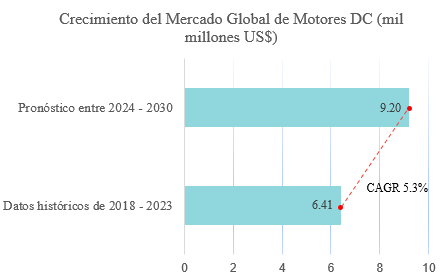
\includegraphics[width=0.6\textwidth]{CHPTRS/CH01_INT/Fig/01_EstudioMercado.png}
    % \caption{Estudio de mercado sobre motores \ac{DC} obtenido de un estudio de la consultora Maximize Market Research \textcite{estadistica_motorDC}}
    % \label{fig:estadistica_problemática}
    % \end{figure}

    
    \begin{figure}[!ht]
    \centering
    \begin{tabularx}{\linewidth}{>{\centering\arraybackslash}X}
        % Fila 1: imagen
        \begin{subfigure}[t]{0.6\linewidth}
            \centering
            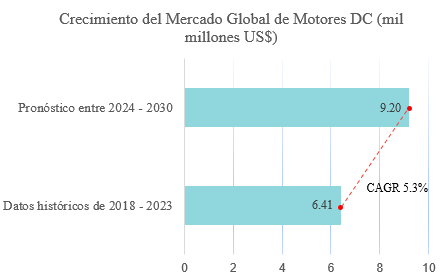
\includegraphics[width=\linewidth]{CHPTRS/CH01_INT/Fig/01_EstudioMercado.png}
        \end{subfigure}
        \\[2mm]
        % Fila 2: nota
        \begin{subfigure}[t]{\linewidth}
            \caption*{\textit{Nota: Figura elaborada a partir de datos de \textcite{estadistica_motorDC}.}}
        \end{subfigure}
    \end{tabularx}
    \caption{Estudio de mercado sobre motores \ac{DC} .}
    \label{fig:estadistica_problemática}
\end{figure}

        
    En el campo de la ingeniería mecatrónica, los motores \ac{DC} son ampliamente utilizados debido a su capacidad para proporcionar un control preciso de velocidad y torque, características esenciales en proyectos de robótica y automatización de procesos \parencites{est_matlab_art_mexicano}. Dos proyectos mecatrónicos relevantes donde se utilicen estos componentes, se presentan a continuación. Ambos proyectos son investigaciones desarrolladas por la empresa \textcite{maxon_group}, reconocida por su especialización en el diseño, desarrollo y fabricación de motores eléctricos de alta calidad.  
    
    El primero de estos proyectos es un robot humanoide llamado Romeo, accionado exclusivamente por motores \ac{DC} de esta empresa. Este robot, ilustrado en la Figura \ref{fig:romeo}, está diseñado para asistir a personas de edad avanzada. Romeo está equipado con 37 motores de alta precisión que controlan sus articulaciones, permitiéndole desplazarse, interactuar y colaborar en las tareas del hogar que, debido a problemas de salud u otras limitaciones, los adultos mayores no puedan realizar.
    
    El segundo proyecto está relacionado con el rover \textit{Perseverance}, diseñado para la exploración y navegación en Marte. En colaboración con la NASA, la empresa \textcite{maxon_group} fue responsable de probar el sistema del rover \textit{Perseverance}, el cual cuenta con diez motores eléctricos que realizan funciones críticas. Entre las funcionalidades que realiza este rover se encuentra el accionar el brazo robótico encargado de transferir muestras entre estaciones, además de sellar y posicionar los contenedores de estas muestras. El rover \textit{Perseverance} se presenta en la Figura \ref{fig:perseverance}.    
%%%%%%%%%%%%%%%%%%%%%%%%%%%%%%%%%%%%%%%%%%%%%%%%%%%%%%%%%%%%%%%%%%%%%%%%%%%%%%%%%%
% NOTA: Para usar una figura al lado de otra se puede usar el paquete \tabularx, la idea es:
%       COL-1     COL-2
%   |----------*-----------*
%   | fig.A    | fig.B     |  FILA-1
%   |----------*-----------*
%   |caption a | caption b |  FILA-2
%   |label a   | label b   |
%   |----------*-----------*
%   |Nota a    | Nota b    |  FILA-3
%   |----------*-----------*
%   caption figura en general
%   label Figura en general.
\begin{figure}[!ht]
    \begin{tabularx}{\linewidth}{*{2}{>{\centering\arraybackslash}X}}
        % FILA-1, COL-1.
        \begin{subfigure}[t]{0.45\textwidth}
            \centering
            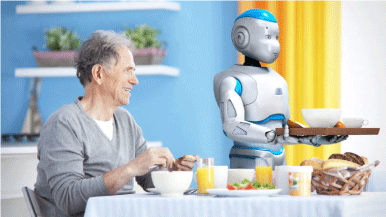
\includegraphics[width=.9\linewidth]{CHPTRS/CH01_INT/Fig/02a_Maxon-Romeo.png}
            %\label{fig:romeo} %LABEL ESTA DESPUES
        \end{subfigure}
        & %Nueva Columna, es decir: % FILA-1, COL-2
        \begin{subfigure}[t]{0.45\textwidth}
            \centering
            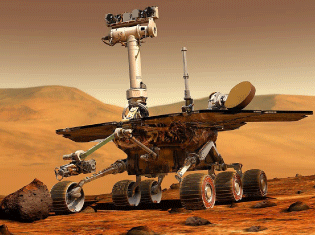
\includegraphics[width=.68\linewidth]{CHPTRS/CH01_INT/Fig/02b_Perseverance.png}
        \end{subfigure}
        \\ %Nueva Fila, es decir: % FILA-2, COL-1
        \begin{subfigure}[t]{0.8\linewidth}
            \caption{Imagen referencial del robot humanoide Romeo}
            \label{fig:romeo}
        \end{subfigure} 
        & %Nueva Columna, es decir: % FILA-2, COL-2
        \begin{subfigure}[t]{0.8\linewidth}
            \caption{Imagen referencial del rover \textit{Perseverance}}
            \label{fig:perseverance}
        \end{subfigure}
        \\ %Nueva Fila, es decir: % FILA-3, COL-1
        \begin{subfigure}[t]{\linewidth}
            \caption*{\textit{Nota: Figura tomada de la página oficial de \linebreak\textcite{maxon_group}}}
        \end{subfigure} 
        & %Nueva Columna, es decir: % FILA-3, COL-2
        \begin{subfigure}[t]{\linewidth}
            \caption*{\textit{Nota: Figura tomada de la página oficial de \linebreak\textcite{maxon_group}}}
        \end{subfigure}
    \end{tabularx}
    \caption{Ejemplos de aplicaciones reales que utilizan motores \ac{DC}}
    \label{fig:figuraEnGeneral}
\end{figure}
%%%%%%%%%%%%%%%%%%%%%%%%%%%%%%%%%%%%%%%%%%%%%%%%%%%%%%%%%%%%%%%%%%%%%%%%%%%%%%%%%
    Para ambos proyectos es fundamental el uso de motores que cumplan con los más altos estándares de calidad, los cuales son previamente sometidos a pruebas en laboratorios altamente especializados. Sin embargo, en el contexto peruano no se dispone de servicios de caracterización de motores eléctricos. Según el profesor Joaquín Gonzales, docente de Máquinas Eléctricas de la \ac{PUCP} e integrante del Centro de Investigación Arvico, “en el Perú, simplemente se opta por comprar \ac{HW} que permita el control de motores DC” (J. Gonzales, comunicación personal, 2024). 
    
    Por todo lo expuesto es conveniente conocer con exactitud los parámetros eléctricos y mecánicos de un motor \ac{DC}, debido a que estos determinan la respuesta del motor y, en consecuencia, influyen en la eficiencia y precisión de este. Además, existen \ac{SW} como \textcite{etap} o MATLAB que permiten realizar estas estimaciones de manera precisa. Sin embargo, todo esto implica un alto costo económico y, aunque son opciones eficaces, no siempre son viables para proyectos de menor escala o presupuestos limitados, lo que resalta la necesidad de alternativas más accesibles.
     
   La principal motivación de este trabajo de investigación es proporcionar a estudiantes de ingeniería mecatrónica y carreras afines una máquina capaz de caracterizar motores DC, facilitando su uso en proyectos y prácticas académicas. Esto fomenta el desarrollo de técnicas de control más precisas con estos componentes durante una etapa de aprendizaje, lo cual puede resultar valioso al integrarse a la industria. Asimismo, en el ámbito industrial, se espera que esta solución sea útil para empresas en el Perú que requieran asesoramiento o herramientas de control de calidad para los motores empleados en aplicaciones de automatización y control, considerando que, como se mencionó, en el país no existe el \textit{know-how} necesario para la caracterización de motores.

    % \section{Propuesta de solución}
    % \label{sec:CH01_Propuesta}
    % Este trabajo se enfocará en el diseño e implementación de un sistema mecatrónico para la estimación de parámetros de motores \ac{DC}. El sistema estará compuesto por dos partes, una de \ac{HW} y otra de \ac{SW}. La primera se encargará del acondicionamiento de señales y la recolección de datos, que luego serán procesados por el algoritmo de estimación de parámetros. La segunda consistirá en el desarrollo del \ac{SW}, el cual se llevará a cabo, inicialmente, en la plataforma MATLAB. Se implementará un algoritmo capaz de estimar los parámetros de los motores \ac{DC}, para ello se desarrollará una interfaz gráfica de usuario \ac{GUI} que permita procesar, visualizar y verificar la precisión del algoritmo. La solución será semi-automatizada, ya que existen motores con diferentes rangos de voltaje y dimensiones. Por lo tanto, se espera que el usuario ajuste manualmente el sistema para adaptarlo al motor que será analizado y en este caso la solución será validada con motores de hasta 12 voltios.
    
    \section{Objetivos}
\label{sec:CH01_Objetivos}
El presente trabajo de investigación tiene como objetivo principal, implementar y validar un diseño de un banco de pruebas para la estimación de  parámetros de motores \ac{DC}. Para lograr este propósito se han definido cinco objetivos específicos, los cuales permitirán estructurar y guiar el desarrollo de la solución óptima.

\subsection{Objetivo general}
El objetivo general es diseñar e implementar un sistema mecatrónico para la estimación de parámetros de motores \ac{DC} utilizando la metodología VDI 2221 y VDI 2206 \autocite{vdi2206} \autocite{vdi2221} y se espera tener, según los niveles de \ac{TRL}, una solución con un nivel de madurez tecnológica TRL4 \autocite{trl}, luego de las respectivas validaciones.

\subsection{Objetivos específicos}
\begin{itemize}
    \item Diseñar el subsistema mecánico del banco: piezas y acoples para el censado de velocidad angular con el encoder elegido, adaptables a las distintas geometrías y ejes de motores en el rango de $12$\,V; soportes de prueba para el motor; un chasis que sirva para conectar correctamente la alimentación de la máquina, del motor y los cables que tendrán los datos del proceso de censado; y una carcasa que indique al usuario si el banco está encendido y soporte todos los componentes de la solución final. Para ello, se utilizarán estándares para los soportes de motores DC, se seleccionarán los conectores y luces de indicación para tener en cuenta las dimensiones de estos componentes, se procederá a medir correctamente y, apoyados con un \ac{SW} de diseño \ac{CAD}, se brindará la correcta posición de todos los componentes, diseñando en el \ac{SW} \ac{CAD} un acople de acuerdo a las necesidades de geometría de los motores que se utilizarán. Para que, todo esto se utilice con la finalidad de apoyar a los demás subsistemas como el electrónico, que necesitará que algunos componentes estén fijos durante las pruebas como el encoder para censar la velocidad, o los conectores de potencia y de información que se conectarán a la computadora donde se realizará la estimación.

    \item Seleccionar los componentes necesarios para el correcto control y comunicación entre el \ac{HW} físico y el \ac{SW} con el algoritmo de estimación, por medio de una \ac{PCB} de control y otra \ac{PCB} dedicada al acondicionamiento y censado de las principales variables del motor. Para ello, se investigarán circuitos que permitan la conexión entre reguladores de voltaje, interfaces y módulos de comunicación, sensores de velocidad, \textit{drivers} para probar el motor y un microcontrolador capaz de controlar toda la experiencia de toma de datos con la información proporcionada por la \ac{GUI}. Todo ello deberá será de suma importancia debido a que el dominio electrónico se encargará de brindar los datos que servirán para la estimación de los parámetros del motor que se quiera caracterizar.

    \item Desarrollar el \ac{SW} que implemente un algoritmo de identificación de parámetros en línea mediante una \ac{GUI} y controle el \ac{HW} del banco de pruebas vía Ethernet. Para ello, se programará la \ac{GUI} para configurar ensayos, enviar comandos al microcontrolador, automatizar la adquisición, visualizar resultados y registrar datos. Para que la identificación se ejecute en línea de forma confiable, se asegurará la comunicación entre \ac{HW} y \ac{SW} eligiendo correctamente el \ac{HW} necesario para ello en los dominios previamente mencionados.

    \item Validar la solución propuesta mediante indicadores cuantitativos de desempeño en al menos dos motores con sus respectivas fichas técnicas en el rango de $12$\,V. A su vez se busca comparar la estimación brindada por el algoritmo a implementar con métodos existentes de estimación de parámetros de motores \ac{DC} descritos en la literatura, considerando costos de implementación y exactitud. 
\end{itemize}
            
    \section{Alcance}
    \label{sec:Alcance}
    Se busca que la solución final alcance un nivel de madurez tecnológica TRL4 \autocite{trl}. Asimismo, se estimará el costo de fabricación del prototipo con el fin de evaluar su viabilidad técnica y económica. Los resultados se validarán mediante métodos de identificación de parámetros descritos en el capítulo \ref{ch:CH02}. Toda investigación y las aproximaciones propuestas se basan en el modelo lineal de los motores de corriente continua presentado en dicho capítulo. Se busca implementar todo el \ac{HW} en su totalidad del concepto ganador y su integración con el \ac{SW} del diseño; de no ser posible culminar esta integración, se dividirá en dos etapas: sensado de datos con el \ac{HW} diseñado y  estimación de parámetros en forma \textit{offline}. Durante el diseño de la solución óptima se optó por indicar que el usuario deberá brindar una fuente externa de acuerdo al voltaje nominal del motor a ensayar. Esta decisión se justifica en el capítulo \ref{ch:CH03}, dedicado al diseño conceptual del prototipo.
    % Cambiar el título de la tesis, al final se compararán los resultados entre motores con y sin caja reductora para ver si varía (eso puede ir en pruebas en alguno de los capítulos de diseño o en Anexos)
    
    \section{Metodología}  
    En el desarrollo de este trabajo de investigación se usará la metodología VDI 2221 y VDI 2206, ambas desarrolladas por la ``Sociedad de Ingenieros Alemanes'' \autocite{vdi2206}. 
    Según lo descrito anteriormente, se organizará el documento de la siguiente manera:
    \begin{itemize}
        \item En el capítulo \ref{ch:CH02} se presentará al lector los conceptos teóricos detrás de la estimación de parámetros de motores \ac{DC}. Seguidamente se presentará el modelo matemático de un motor \ac{DC} y los parámetros que conforman la dinámica del mismo, a su vez de detallarán los algoritmos más usados para la caracterización de motores \ac{DC}, según \autocite{Electronics}.
        
        \item En el capítulo \ref{ch:CH03} se abordará el diseño conceptual del sistema a desarrollar, presentando una lista de requerimientos que delimitará el funcionamiento que deberá cumplir la solución diseñada en los capítulos posteriores. Esta lista expresa principalmente requerimientos cuantitativos, lo que permitirá realizar un seguimiento para verificar que se cumplan los valores correspondientes. Para su elaboración, se investigaron antecedentes de trabajos afines y se entrevistó al actual director de la Maestría en Control y Automatización de la \ac{PUCP}, quien arguye con su perspectiva y experiencia para acotar los requerimientos del sistema presentados en esta tesis.
        
        \item En el capítulo 3 se presentarán empresas de renombre que ofrecen motores DC junto con sus respectivas especificaciones, así como software destinado a la estimación de parámetros. Además, se analizarán artículos y papers de aplicaciones previas que expongan resultados de soluciones utilizadas para estimar parámetros de motores DC. Asimismo, se incluirá una lista de los componentes necesarios para la estimación de parámetros, como sensores de corriente, encoders para medir la velocidad angular del motor, entre otros componentes.
        
        \item A su vez, en el capítulo \ref{ch:CH03} se identificarán las señales de entrada del sistema y se definirán las salidas que contará el sistema base de la cual partirá la estructura de funciones del sistema. Luego de ello se presentarán los componentes/medios necesarios para las pruebas con los motores y la adquisición data relevante para el procesamiento del algoritmo de estimación. Se propondrán al menos tres soluciones, conforme a la norma, y que serán evaluadas mediante un análisis técnico-económico, en base a ello se elegirá un sólo concepto de solución que se tomará como base para el diseño del estimador de parámetros. 
        
        \item Posteriormente, se procederá a diseñar cada una de las funciones de los dominios mecánicos, electrónicos, software y de control que contará la solución óptima elegida para, finalmente, ser implementada y testeada con diferentes tipos de motores para comprobar la estimación de parámetros.
        
        \item Finalmente, se presentarán los resultados obtenidos por el concepto de solución diseñado. En caso no se llegase a cumplir con todos los objetivos propuestos o los requerimientos brindados, se optará por dar recomendaciones o alternativas que aseguren la correcta estimación de parámetros de motores \ac{DC}.
    \end{itemize}
    
    
            \cleardoublepage
\chapter{Estado del arte}
\ihead[]{Capítulo 2: Estado del arte}
\label{ch:CH02-Estado-del-Arte}
%%%%%%%%%%%%%%%%%%%%%%%%%%%%%%%%%%%%%%%%%%
En este capítulo se presenta una revisión de \ac{SW} comerciales, empresas que se encargan de la venta de motores con sus respectivas especificaciones y trabajos de investigación relacionados con la caracterización de motores \ac{DC}. %asimismo se presentan tecnologías que serán tomados en cuenta para los conceptos de solución en capítulos posteriores
\section{Softwares comerciales}
    Se destacan 2 \ac{SW} que facilitan la estimación de parámetros de motores \ac{DC}, Con dichos \ac{SW} se piensa comparar los resultados que se obtengan con la solución que se planteará el capítulos posteriores.
    \subsection{Software ETAP}
        \ac{ETAP} es un \ac{SW} especializado en el análisis de sistemas eléctricos de potencia. Dentro de sus módulos, cuenta con un apartado dedicado a la estimación de parámetros de motores. Para ello, según lo indica la página oficial \autocite{etap}, utiliza técnicas de estimación matemática y ajuste de curvas para esta tarea, y requiere sólo datos de rendimiento del motor. También permite generar informes detallados y gráficos de los resultados, facilitando análisis de torque, corriente y eficiencia del motor \autocite{etap}. En la Figura \ref{fig:CH02_SW_ETAP} se presenta la interfaz del \ac{SW} referente a la caracterización de motores.
        \begin{figure}[!ht]
        \centering
        \begin{tabularx}{\linewidth}{>{\centering\arraybackslash}X}
            % Fila 1: imagen
            \begin{subfigure}[t]{0.5\linewidth}
                \centering
                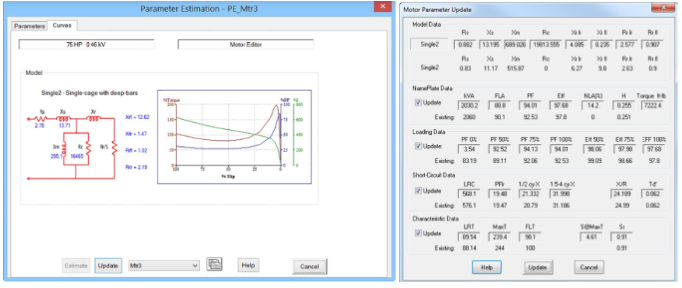
\includegraphics[width=\linewidth]{CHPTRS/CH02_SA/Fig/01_SWEtap.PNG}
            \end{subfigure}
        \end{tabularx}
        \caption{Imágenes extraídas de la página oficial de ETAP}
        \label{fig:CH02_SW_ETAP}
        \end{figure}
    
    \subsection{MATLAB/Motor Control Blockset}
        La herramienta \ac{MCB}, brindada por el \ac{SW} Matlab es utilizada para el diseño, simulación y prueba de sistemas de control de motores \ac{DC}. Entre sus principales funciones se destaca la simulación de motores con diferentes parámetros para analizar su comportamiento bajo diversas condiciones, el diseño de controladores de velocidad y torque utilizando técnicas de control de lazo cerrado y brinda documentación de proyectos y aplicaciones brindadas por la comunidad de temas relacionados con la estimación de motores \autocite{mathworks_motor_estimation}. \\
        \begin{figure}[!ht]
        \centering
        \begin{tabularx}{\linewidth}{>{\centering\arraybackslash}X}
            % Fila 1: imagen
            \begin{subfigure}[t]{0.5\linewidth}
                \centering
                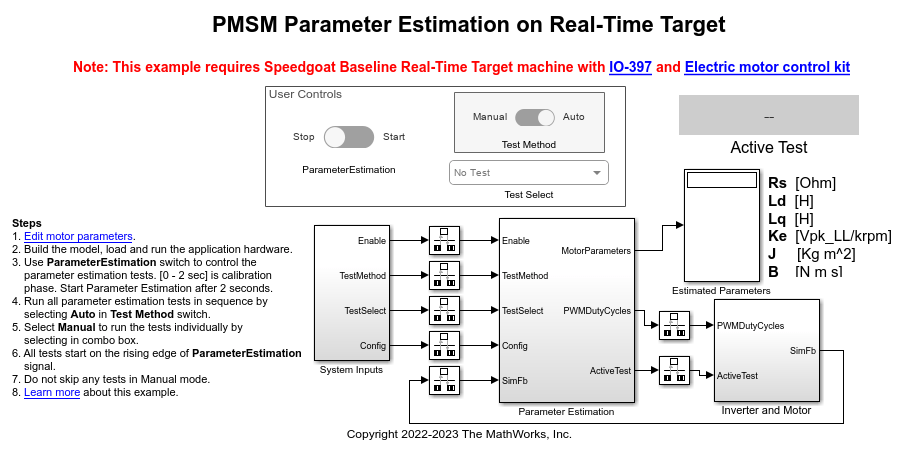
\includegraphics[width=\linewidth]{CHPTRS/CH02_SA/Fig/02_MatlabToolbox.png}
            \end{subfigure}
            \end{tabularx}
            \caption{Imagen extraída de la página de MathWorks \autocite{mathworks_motor_estimation}}
            \label{fig:CH02_SW_ETAP}
        \end{figure}
    A continuación se presenta en la Tabla \ref{tab:comparasion_sw} tabla comparativa entre los dos \ac{SW} presentados, se compararán el precio para adquirir estas herramientas, si cumplen con estimar los parámetros de motor y qué tanta documentación se le brinda al usuario. Toda información en dicha tabla ha sido consultada a las páginas oficiales de cada \ac{SW}.
    % Tabla adaptada con la plantilla "tabla_comparativa" (3 columnas)
    % NOTA: Ajusta {w1}+{w2}+{w3} <= 1 para evitar warnings.
    \begin{longtblr}[theme=pucp,
          label   = {tab:comparasion_sw},
          caption = {Comparación entre los dos \ac{SW} mencionados},
        ]{
          colspec   = {X[c,m]X[c,m]X[c,m]},
          column{1} = {wd=0.20\textwidth},
          column{2} = {wd=0.40\textwidth},
          column{3} = {wd=0.40\textwidth},
          rowhead = 1,
          rowfoot = 0,
          hlines,
          vlines,
        }
        Característica & \ac{ETAP} & MATLAB \textit{toolbox} \\
        Precio de la licencia
        & El \ac{SW} \ac{ETAP} tiene un precio modular, por lo que se deben comprar módulos separados para distintas características. \ac{ETAP} no publica precios directos; es necesario solicitar una cotización.
        & MATLAB opera con licencias cuyo precio varía según el tipo (individual, académico, etc.). La licencia anual base de MATLAB (con acceso a todas las herramientas) es de \$2{,}150, y el \ac{MCB} se vende por separado (puede llegar a \$1{,}500). El plan estudiantil más económico indicado por \textcite{mathworks_motor_estimation} cuesta \$55. \\
        Estimación de parámetros del motor
        & \ac{ETAP} se especializa en análisis de sistemas eléctricos de potencia e incluye un apartado para estimar parámetros de motores \ac{DC} como resistencia, inductancia y par.
        & MATLAB/\ac{MCB} ofrece herramientas completas para estimación de parámetros de motores, con entornos de simulación e interfaces de hardware para diseño de control y pruebas en tiempo real. \\
        Soporte y documentación
        & \ac{ETAP} ofrece soporte extenso: ayuda en vivo, capacitaciones, seminarios web y foro dedicado.
        & MATLAB/\ac{MCB} cuenta con documentación completa, foros de usuarios, soporte técnico de MathWorks y abundantes tutoriales en línea. \\
    \end{longtblr}

\section{Empresas de confianza}
    En esta sección, se analizarán dos empresas internacionales que ofrecen a sus clientes los parámetros técnicos de sus motores en hojas de especificaciones antes de la compra de sus productos.
    \subsection{Maxon}
        Maxon ofrece soluciones de sistemas de accionamiento mecatrónico y uno de sus componentes de mayor interés son los motores \ac{DC}. Estos componentes se destacan por su alta precisión, fiabilidad y adaptabilidad a diversas aplicaciones industriales, médicas, aeroespaciales y de movilidad. Los motores \ac{DC} de Maxon se usan en entornos donde la identificación de parámetros precisos, como torque, velocidad y eficiencia, es crítica para un rendimiento óptimo, especialmente en tareas de automatización y robótica \autocite{maxon_group}. Adicionalmente, buscando en la página oficial, al cotizar un motor de esta marca puedes realizar distintas combinaciones de componentes como \textit{drivers}, encoders pero lo principal es que por cada motor, te brindan una lista de especificaciones, de las cuales se destacan las que ayudarán al control del motor. En la Figura \ref{fig:CH03_MOTOR_MAXON} se muestra la cotización de uno de los modelos de motor \ac{DC} y en la Tabla \ref{tab:motor_maxon} se brindan las especificaciones de dicho motor.
    
    \begin{figure}[H]
        \centering
        \begin{tabularx}{\linewidth}{>{\centering\arraybackslash}X}
            % Fila 1: imagen
            \begin{subfigure}[t]{0.5\linewidth}
                \centering
                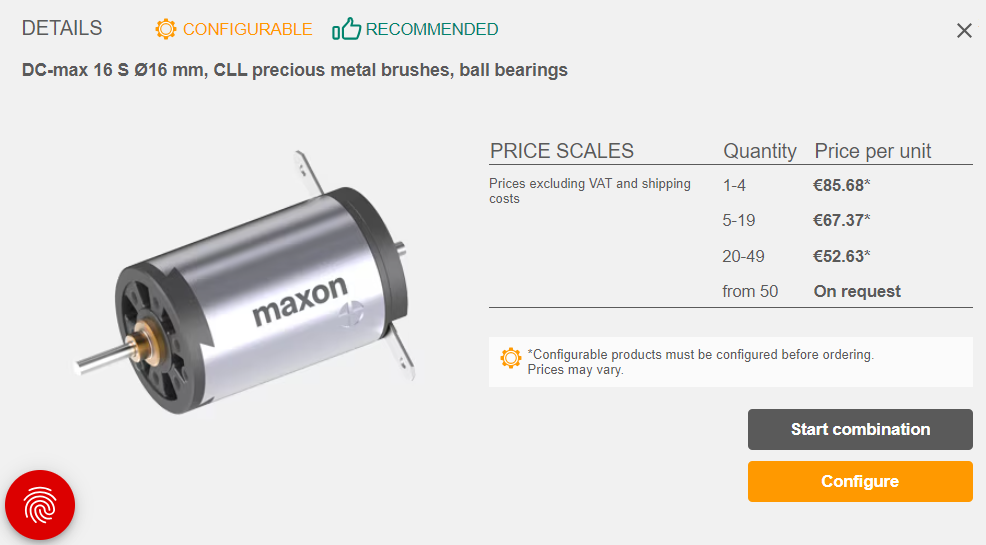
\includegraphics[width=\linewidth]{CHPTRS/CH02_SA/Fig/03_MaxonMotor.PNG}
            \end{subfigure}
        \end{tabularx}
        \caption{Imagen referencial del motor cotizado en la página de MAXON}
        \label{fig:CH03_MOTOR_MAXON}
    \end{figure}
    \begin{table}[H]
        \centering
        \caption{Parámetros brindados por la empresa MAXON al momento de elegir un motor\\(modelo DC-max 16)}
        \begin{tblr}{
              cell{1}{3} = {c},
              cell{2}{3} = {c},
              cell{3}{3} = {c},
              cell{4}{3} = {c},
              cell{5}{3} = {c},
        }
        \hline
        Características              & Valor            &  \\
        \hline
        Resistencia terminal         & \SI{4.1}{\ohm}   &  \\
        Inductancia terminal         & \SI{0.14}{\mH}   &  \\
        Constante de par             & 7,19 mNm/A       &  \\
        Constante de velocidad       & 1330 rpm/V       &  \\
        Gradiente de velocidad/par   & 758 rpm/mNm      &  \\
        Constante de tiempo mecánico & 8,87 ms          &  \\
        Inercia del rotor            & 1,12 $gcm^2$     &
        \end{tblr}
        \caption*{\small\textit{Nota: Información adaptada de un motor cotizado en la página de \href{https://www.maxongroup.com/es-es}{Maxon}, revisada el día 25 de setiembre del 2024 \autocite{maxon_group}}}
        \label{tab:motor_maxon}
    \end{table}

\subsection{Zhaowei}
    ZHAOWEI es una empresa que se especializa en el diseño, desarrollo y fabricación de motores \ac{DC} con escobillas, así como en sistemas de transmisión y soluciones personalizadas para la industria. Se enfoca principalmente en la venta de motores de alta precisión y componentes relacionados afines para el accionamiento y medición de parámetros de estos \autocite{zhaowei_dc_motor} Lo destacable de la empresa es que, al igual que fabricantes como \textcite{zhaowei_dc_motor}, proporcionan los parámetros técnicos detallados de sus motores antes de la compra, lo cual es importante para que los clientes puedan evaluar si el motor cumple con sus requisitos específicos. Algo a detallar es que al momento de ingresar a cotizar un motor, dichos parámetros se encuentran ligados a una tolerancia de casi el 20 \% para la mayoría de estos y en algunos casos no muestran los valores de algunos parámetros. En la Figura \ref{fig:CH03_MOTOR_ZHAOWE} se muestran los principales parámetros de uno de los modelos de motor \ac{DC} de la página principal de esta empresa y en la Tabla \ref{tab:motor_zhaowei} se muestran los valores de los parámetros del motor cotizado.

    \begin{figure}[H]
        \centering
        \begin{tabularx}{\linewidth}{>{\centering\arraybackslash}X}
            % Fila 1: imagen
            \begin{subfigure}[t]{0.8\linewidth}
                \centering
                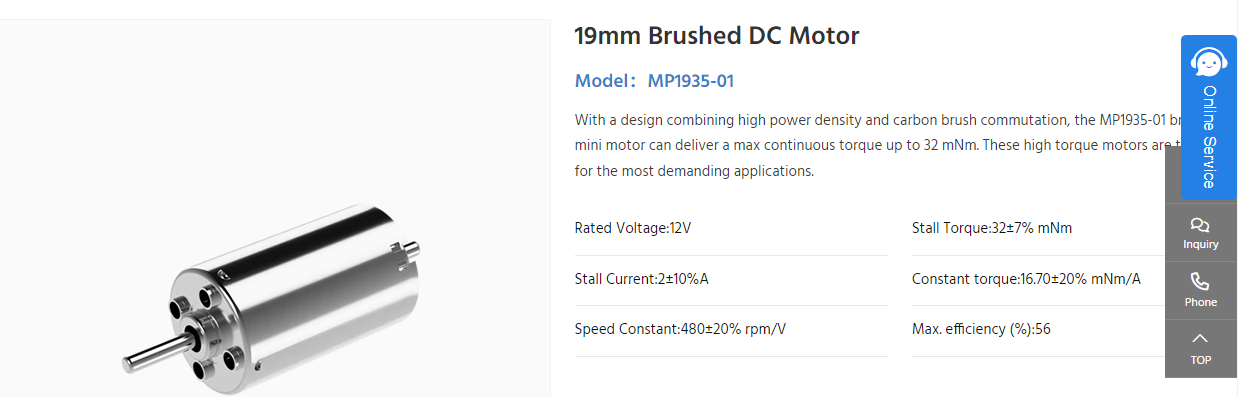
\includegraphics[width=\linewidth]{CHPTRS/CH02_SA/Fig/04_ZhaoweiMotor.PNG}
            \end{subfigure}
        \end{tabularx}
        \caption{Imagen referencial del motor cotizado en la página de Zhaowei}
        \label{fig:CH03_MOTOR_ZHAOWE}
    \end{figure}
    \begin{table}[H]
        \centering
        \caption{Parámetros brindados por la empresa ZHAOWEI del motor cotizado en su página web}
        \begin{tblr}{
          cell{1}{3} = {c},
          cell{2}{3} = {c},
          cell{3}{3} = {c},
          cell{4}{3} = {c},
          cell{5}{3} = {c},
        }
        \hline
        Características                    & Valor            &  \\
        \hline
        Resistencia terminal de fase       & \SI{4.5}{\ohm}   &  \\
        Inductancia terminal de fase       & \text{N.A.}      &  \\
        Constante de par                   & 13,1 mNm/A       &  \\
        Constante de velocidad             & 684 rpm/V        &  \\
        Gradiente de velocidad/par         & 243,5 rpm/mNm    &  \\
        Constante de tiempo mecánico       & -- ms            &  \\
        Inercia del rotor                  & 4 $gcm^2$        &
        \end{tblr}
        \caption*{\small\textit{Nota: Información adaptada de un motor cotizado en la página de \href{https://es.zwgearbox.com/}{Zhaowei}, revisada el día 25 de setiembre del 2024 \autocite{zhaowei_dc_motor}}}
        \label{tab:motor_zhaowei}
    \end{table}


Para la validación de los resultados del estimador diseñado, se utilizará un motor proveniente de alguna de las dos empresas mencionadas, dado que estas empresas proporcionan una hoja técnica con los valores de los parámetros del motor. Además, se planea aplicar métodos empíricos y utilizar algún \ac{SW} para comparar cuál de estas tres metodologías ofrece resultados más cercanos a la respuesta real y determinar cuál de ellas es la mejor opción para hallar los parámetros.
 
\section{Artículos académicos:}
    A continuación se presentan 3 artículos enfocados en caracterizar motores de corriente continua, cada uno de ellos muestra distintas técnicas para lograr estimar los modelos de motores \ac{DC}, pero lo que se comparte en cada una de estas publicaciones es la efectividad de sus modelos al compararlos con los datos obtenidos por un motor real. 
    \subsection{Identificación de parámetros de motores de \ac{DC} usando respuesta en frecuencia}
        En este artículo\textcite{vollmecke_parameter_identification} propone la estimación de parámetros de motores \ac{DC} utilizando la respuesta en frecuencia para reconstruir la función de transferencia del motor mediante la aproximación de los polos que caracterizan la dinámica del sistema. En la Figura \ref{fig:CH03_Diagrama_Bode} se presenta el diagrama de Bode del sistema una vez determinados los polos. Posteriormente, estos se emplean para calcular los parámetros del motor utilizando las constantes de tiempo de respuesta del sistema: en el dominio eléctrico, para determinar los valores de la resistencia e inductancia; y en el dominio mecánico, para calcular la inercia y el factor de viscosidad del eje del motor.
        \begin{figure}[h!]
            \centering
            \begin{tabularx}{\linewidth}{>{\centering\arraybackslash}X}
                % Fila 1: imagen
                \begin{subfigure}[t]{0.8\linewidth}
                    \centering
                    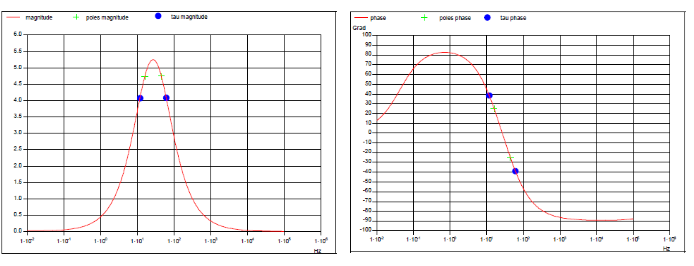
\includegraphics[width=\linewidth]{CHPTRS/CH02_SA/Fig/05_RespFrecuencia.PNG}
                \end{subfigure}
            \end{tabularx}
            \caption{Diagrama de Bode que muestra la identificación de los polos del motor}
            \label{fig:CH03_Diagrama_Bode}
        \end{figure}

    \subsection{Identificador algebraico de parámetros mecánicos de un motor \ac{DC}}
        En un artículo publicado por Academia Journals, se presenta un método económico para identificar únicamente los parámetros mecánicos de motores \ac{DC}, específicamente la inercia del eje y el coeficiente de viscosidad. Según \textcite{parametros_mecanicos}, se implementa el modelo del motor \ac{DC} junto con un identificador algebraico de parámetros en MATLAB/SIMULINK, como se ilustra en la Figura \ref{fig:CH03_ESTIMADOR_MECANICO}, donde se simula el comportamiento del sistema en condiciones ideales. Para la implementación experimental, se utiliza el circuito mostrado en la misma figura, en el cual un microcontrolador Arduino UNO procesa las mediciones de velocidad y corriente para determinar los parámetros del motor \ac{DC}, enviándolos posteriormente a MATLAB/SIMULINK. Un sensor infrarrojo con \textit{encoder} mide la velocidad del motor, mientras que un circuito simple con una resistencia permite medir la corriente.
        \begin{figure}[H]
            \centering
            \begin{tabularx}{\linewidth}{>{\centering\arraybackslash}X}
                % Fila 1: imagen
                \begin{subfigure}[t]{0.6\linewidth}
                    \centering
                    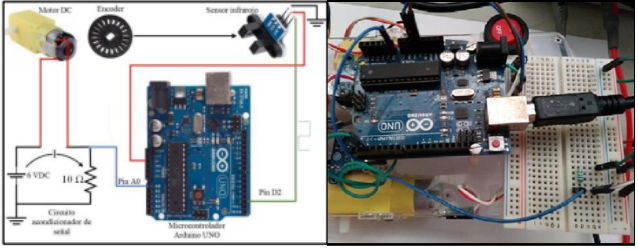
\includegraphics[width=\linewidth]{CHPTRS/CH02_SA/Fig/06_Antecedente1.PNG}
                \end{subfigure}
            \end{tabularx}
            \caption{Implementación experimental para la toma de datos}
            \label{fig:CH03_ESTIMADOR_MECANICO}
        \end{figure}

        A continuación se presentan los resultados de la estimación que obtuvo \textcite{parametros_mecanicos}, donde se destaca que al ser una implementación con componentes bastante económicos y sin la ayuda de filtros, sólo se logra estimar correctamente el coeficiente de viscosidad, más no el momento de inercia del eje del motor debido a que no se filtró correctamente el ruido en la toma de datos. Esto como se logra ver en la comparación de parámetros entre el real y el que fue estimado. El efecto de la inercia nunca llega a converger con el resultado obtenido por el estimador. Esto se presenta en la Figura \ref{fig:CH03_RESULTADOS_MECANICOS}.
        \begin{figure}[H]
            \centering
            \begin{tabularx}{\linewidth}{>{\centering\arraybackslash}X}
                % Fila 1: imagen
                \begin{subfigure}[t]{0.6\linewidth}
                    \centering
                    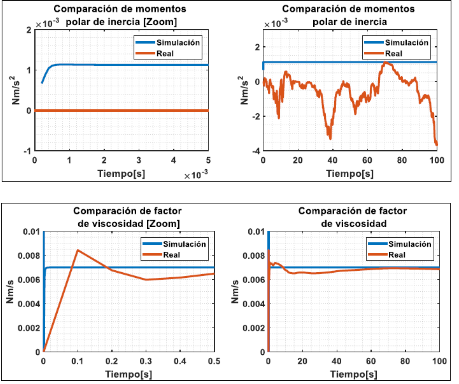
\includegraphics[width=\linewidth]{CHPTRS/CH02_SA/Fig/07_Antecedentes2.PNG}
                \end{subfigure}
            \end{tabularx}
            \caption{Resultados de la estimación de parámetros mecánicos}
            \label{fig:CH03_RESULTADOS_MECANICOS}
        \end{figure}

    \subsection{Sistema de identificación paramétrica para motores \ac{DC} usando método de mínimos cuadrados}
        El siguiente artículo proviene de una publicación de 2 institutos mexicanos y trata de un sistema diseñado para identificar los parámetros que describen la función de transferencia de un motor de corriente continua. El sistema consta de una tarjeta para la adecuación de señales, una tarjeta de adquisición de datos y una aplicación de computadora que implementa el algoritmo de mínimos cuadrados usando un programa creado en MATLAB. Las señales que requirieron medir incluyen la velocidad angular en radianes por segundo, la corriente de armadura en amperios y el voltaje de alimentación en voltios. Se muestra la relación matemática entre la función de transferencia del motor de corriente continua y las funciones de transferencia de velocidad y corriente. En la Figura \ref{fig:CH03_DIAGRAMA_ESQ_MEX} presenta el diagrama de conexiones que usaron \textcite{est_matlab_art_mexicano} para la adquisición de datos de motores \ac{DC}. Además, en la Figura \ref{fig:CH03_INTERFAZ_MEX} se muestra la interfaz que desarrolló su equipo para realizar la estimación de parámetros del motor.
    \begin{figure}[!ht]
        \begin{tabularx}{\linewidth}{*{2}{>{\centering\arraybackslash}X}}
            % FILA-1, COL-1 (imagen izquierda)
            \begin{subfigure}[t]{0.45\textwidth}
                \centering
                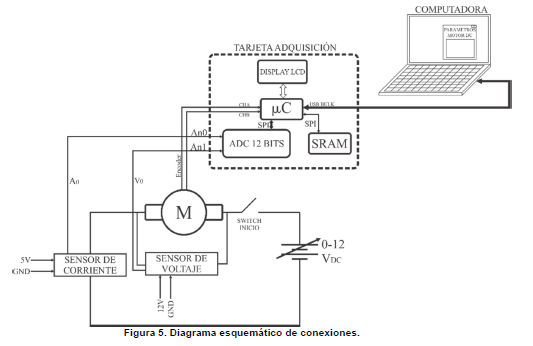
\includegraphics[width=.9\linewidth,height=4cm,keepaspectratio]{CHPTRS/CH02_SA/Fig/08a_DiagramaConexiones.PNG}
            \end{subfigure}
            &
            % FILA-1, COL-2 (imagen derecha)
            \begin{subfigure}[t]{0.45\textwidth}
                \centering
                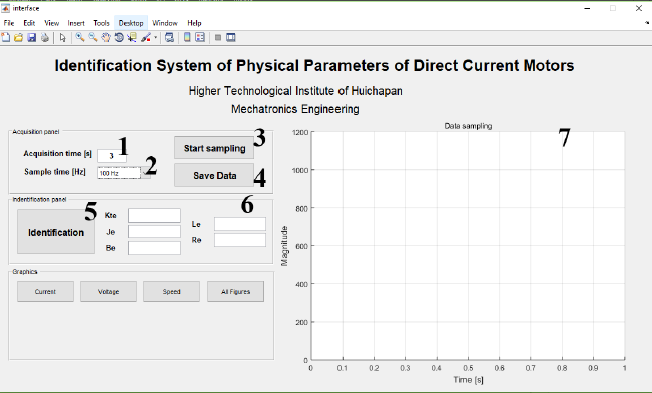
\includegraphics[width=.9\linewidth,height=4cm,keepaspectratio]{CHPTRS/CH02_SA/Fig/08b_Interfaz.PNG}
            \end{subfigure}
            \\
            % FILA-2 (captions individuales)
            \begin{subfigure}[t]{0.8\linewidth}
                \caption{Diagrama esquemático de conexiones para toma de datos de motores \ac{DC}}
                \label{fig:CH03_DIAGRAMA_ESQ_MEX}
            \end{subfigure}
            &
            \begin{subfigure}[t]{0.8\linewidth}
                \caption{Interfaz propuesta para el procesamiento y ejecución del algoritmo de estimación}
                \label{fig:CH03_INTERFAZ_MEX}
            \end{subfigure}
        \end{tabularx}
        \caption{Diseño propuesto por \textcite{est_matlab_art_mexicano} para la estimación de parámetros de motores \ac{DC}}
        \label{fig:figura_con_subfiguras}
    \end{figure}

      \cleardoublepage 
\chapter{Diseño conceptual}
\ihead[]{Capítulo 3: Diseño conceptual}
\label{ch:CH03-Diseno-Conceptual}
%%%%%%%%%%%%%%%%%%%%%%%%%%%%%%%%%%%%%%%%%%
En este capítulo se presentan tres alternativas de conceptos de solución, las cuales han sido elaboradas \lipsum[2]. \cleardoublepage
\chapter{Diseño electrónico del sistema}
\ihead[]{Capítulo 4: Diseño electrónico del sistema}
\label{ch:CH04-Diseno-Electronico}
%%%%%%%%%%%%%%%%%%%%%%%%%%%%%%%%%%%%%%%%%%
En este capítulo se desarrollará el diseño electrónico de los subsistemas del concepto de solución óptima, incluyendo la selección de los componentes necesarios para el funcionamiento del sistema. Asimismo, se establecen las consideraciones de diseño de una \ac{PCB} a medida que integre los componentes definidos, tomando como base las pruebas en prototipo y la documentación técnica de cada componente elegido.
\section{Selección de componentes electrónicos}
    El \ac{HW} del sistema realizará tres tareas principales: energizar el motor de pruebas, sensar sus variables físicas (voltaje, corriente y velocidad angular) y enviar los datos del sensado de variables hacia la interfaz. Por ello, se comenzará realizando la selección de componentes que permitan realizar las tareas.
    \subsection{Selección de microcontrolador}
        Para iniciar el diseño se definirá el microcontrolador a utilizar. Como se presentó en la matriz morfológica \ref{fig:Annex_E_MatrizMorfologica-05-control} del Anexo \ref{an:Anexo_G_MatrizMorfologica}, se consideraron dos opciones: un microcontrolador y una \ac{SBC}. Por criterios de costo expuestos en la sección \ref{sec:solucion_optima}, y dado que durante la experiencia de registro de datos se desarrollará una interfaz de escritorio para controlar el \ac{HW} desde la \ac{PC} del usuario, se descartó la opción de utilizar una \ac{SBC}. En consecuencia, se evalúan tres opciones de microcontroladores comerciales: placas de desarrollo basadas en la familia ATmega (Arduino), el microcontrolador ESP32 y la placa de desarrollo STM32F103C8T6 de la familia de microcontroladores STM32. A continuación, en la Tabla \ref{tab:mcus} se presentan estas tres alternativas para el desarrollo de la PCB de control del \ac{HW} y sus principales características.
        
        \begin{longtblr}[theme=pucp,
          label   = {tab:mcus},
          caption = {Comparativa de microcontroladores para el banco de pruebas (IO, adquisición y conectividad)},
        ]{
          colspec = {X[c,m] X[l,m] X[l,m] X[l,m]}, % 1ª centrada, resto a la izq.
          colsep=3pt,
          row{1}={halign=c},
          rowhead=1, rowfoot=0,
          hlines, vlines,
        }
        Característica
          & 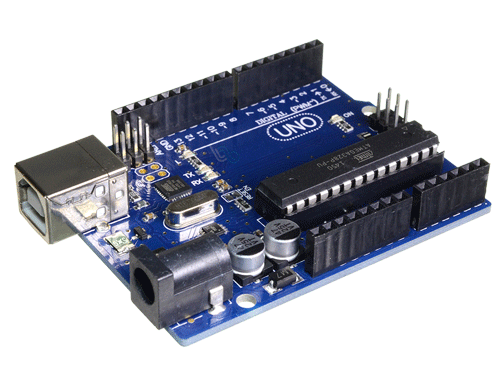
\includegraphics[width=2.5cm]{CHPTRS/CH04_DIS_ELECTRONICO/Componentes/ArduinoUNO.png} Arduino UNO R3 (Atmega328P)
          & \includegraphics[width=2.5cm]{CHPTRS/CH04_DIS_ELECTRONICO/Componentes/DIS_ELEC_01_ChipESP32-32D.jpg} ESP32-WROOM-32D
          & 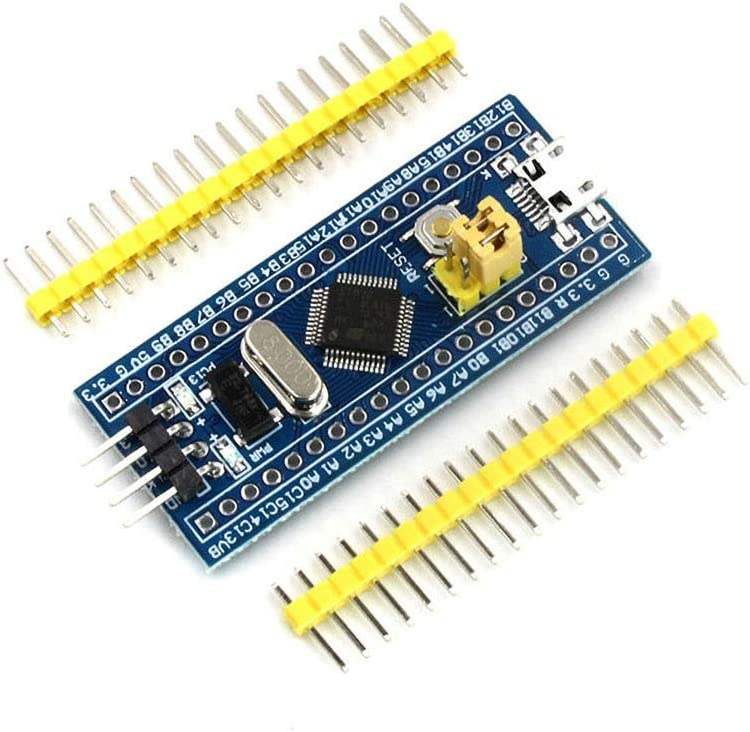
\includegraphics[width=2.5cm]{CHPTRS/CH04_DIS_ELECTRONICO/Componentes/STM32.jpg} STM32F103C8T6\\
        Arquitectura / núcleos
          & AVR 8 bit, 1 núcleo hasta 16\,MHz
          & Xtensa LX6, 2 núcleos hasta 240\,MHz
          & Arm Cortex-M3 32 bit hasta 72\,MHz \\
        Memoria
          & Flash 32\,KB, SRAM 2\,KB, EEPROM 1\,KB
          & SRAM 520\,KB, 4\,MB SPI flash en el módulo
          & Flash 64\,KB (algunas placas 128\,KB); SRAM 20\,KB \\
        ADC / DAC
          & ADC 10 bit (6 canales), sin DAC
          & 2 SAR ADC 12 bit (hasta 18); 2 DAC 8 bit
          & 2 ADC 12 bits (hasta 16 canales); sin DAC \\
        Comunicaciones
          & UART, SPI, $I^2C$
          & SPI, $I^2C$, UART, SDIO, TWAI (CAN 2.0), MAC Ethernet\footnotemark[1]
          & SPI, $I^2C$, USART/UART, CAN 2.0B, USB FS \\
        Temporizadores / PWM
          & 6 salidas PWM
          & LEDC PWM, MCPWM
          & hasta 7 temporizadores (PWM/IC/OC, interfaz de encoder; TIM1 avanzado) \\
        Conectividad RF
          & No cuenta con esta funcionalidad & Wi-Fi 802.11 b/g/n + Bluetooth v4.2 BR/EDR + BLE & No cuenta con esta funcionalidad \\
        Voltaje de operación (IO)
          & 5\,V (IO 5\,V)
          & 3.0 – 3.6\,V (IO 3.3\,V)
          & 2.0 – 3.6\,V (IO 3.3\,V; \emph{algunos pines toleran 5\,V}) \\
        Entorno de desarrollo
          & Arduino IDE
          & ESP-IDF (oficial) / Arduino Core
          & STM32CubeIDE/HAL (opcional Arduino Core STM32) \\
        Precio (moneda local S/)
          & S/ 25 & S/ 30 & S/ 25 \\
        \end{longtblr}
        \footnotetext[1]{Microcontrolador ESP32 incorpora interfaz MAC Ethernet (RMII); sin embargo requiere un PHY externo.}
        % \begin{figure}[H]
        %     \centering
        %     \begin{tabularx}{\linewidth}{>{\centering\arraybackslash}X}
        %         % Fila 1: imagen
        %         \begin{subfigure}[t]{\linewidth}
        %             \centering
        %             \includegraphics[width=0.35\linewidth]{CHPTRS/CH04_DIS_ELECTRONICO/Fig_Componentes/DIS_ELEC_01_ChipESP32-32D.jpg}
        %         \end{subfigure}
        %     \end{tabularx}
        %     \caption{Microcontrolador ESP32-WROOM-32}
        %     \label{fig:black_box}
        % \end{figure}
        Se utilizará el microcontrolador ESP32-32D montado en una placa propia y programable mediante USB-C gracias a un convertidor USB–TTL CH340 configurado a 3.3\,V. El \textit{chip} CH340 ofrece interfaz USB que se enumera como puerto serie virtual y habilita carga de firmware. El diseño de este  Además, el microcontrolador ESP32 aporta doble núcleo (hasta 240\,MHz), SRAM integrada, ADC de 12 bits, temporizadores y periféricos PWM para el control del puente H, además de SPI para los periféricos de adquisición (sensor magnético y módulo Ethernet). En cuanto al \ac{SW}, la plataforma admite FreeRTOS y capacidades de tiempo real, disponibles pero no necesariamente empleadas en este proyecto. La combinación USB-C con CH340 para programación y comunicación serie, junto con las interfaces SPI, PWM y ADC del ESP32, satisface los requisitos del banco de pruebas para el sensado y la transmisión de datos hacia la \ac{PC}.
        \begin{figure}[H]
            \centering
            \begin{tabularx}{\linewidth}{>{\centering\arraybackslash}X}
                % Fila 1: imagen
                \begin{subfigure}[t]{\linewidth}
                    \centering
                    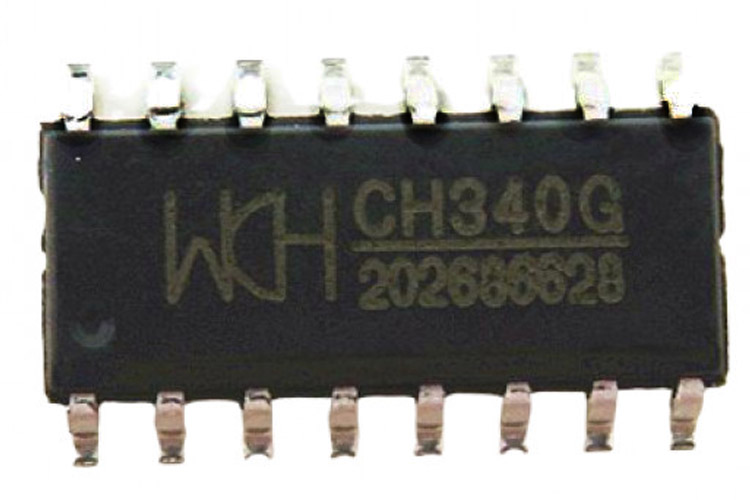
\includegraphics[width=0.4\linewidth]{CHPTRS/CH04_DIS_ELECTRONICO/Fig_Componentes/DIS_ELEC_02a_ChipCH340.jpg}
                \end{subfigure}
            \end{tabularx}
            \caption{Integrado CH340 cargar el programa y de poder comunicarse con el micrcontrolador elegido}
            \label{fig:black_box}
        \end{figure}
    \subsection{Selección de sensor de efecto \textit{hall}}
        Como se mencionó en la sección \ref{sec:solucion_optima} del Capítulo \ref{ch:CH03-Diseno-Conceptual} se utilizarán sensores de efecto \textit{hall} para medir la velocidad angular del motor. Este sensor a elegir debe ser lo suficientemente rápido para medir los cambios en la velocidad del motor, ya que como se puede observar en el Capítulo \ref{ch:CH07_Implementacion}, los motores \ac{DC} son sistemas que reaccionan muy rápido y estabilizan sus variables en poco tiempo (aquí se referenciaran secciones del Capítulo \ref{ch:CH07_Implementacion} que contengan gráficas de velocidad de los motores a probar)
        se seleccionó el TMAG5170 por cuatro razones alineadas al diseño del prototipo:
        \begin{itemize}
        \item Alta razón de muestreo y baja latencia. Su conversión rápida (orden de decenas de \si{\micro\second}) y lectura permiten explotar la capacidad de servicio de interrupciones de la ESP32, de modo que el lazo de adquisición (Cap. \ref{ch:CH07_Implementacion}) estima velocidad angular con retraso despreciable respecto a la dinámica del motor. 
        \item Versatilidad funcional. Aunque el diseño original contemplaba un disco con imanes para detectar flancos (disco con imanes en el eje del motor), la disponibilidad del ángulo (\(0\text{–}360^\circ\)) y la habilitación selectiva de ejes X–Y–Z permiten simplificar el \ac{HW}: se reemplaza el conteo de flancos por medición angular directa del imán montado en el eje. 
        \item Compatibilidad eléctrica y de integración. Su alimentación entre \SI{2.3}{\volt} y \SI{5.5}{\volt} y niveles lógicos referidos a V\textsubscript{CC} facilitan operar con el microcontrolador seleccionado a \SI{3.3}{\volt}. Además, que simplifica el hecho de utilizar una etapa extra de regulación aparte de la que energiza al microcontrolador y los demás módulos. 
        \item Interfaz \ac{SPI} . La comunicación serie síncrona se puede implementar con el microcontrolador seleccionado tanto para la programación del sensor como para recibir los datos de velocidad angular
        \end{itemize}
        \ref{sec:solucion_optima}.
        \begin{figure}[H]
            \centering
            \begin{tabularx}{\linewidth}{>{\centering\arraybackslash}X}
                % Fila 1: imagen
                \begin{subfigure}[t]{\linewidth}
                    \centering
                    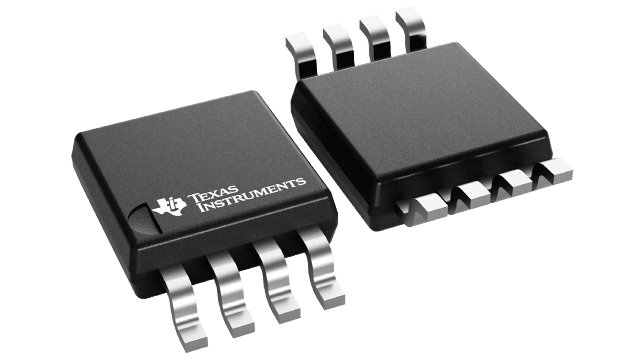
\includegraphics[width=0.4\linewidth]{CHPTRS/CH04_DIS_ELECTRONICO/Fig_Componentes/DIS_ELEC_03a_ChipTMAG.jpg}
                \end{subfigure}
            \end{tabularx}
            \caption{Imagen del sensor de efecto \textit{hall} TMAG5170}
            \label{fig:black_box}
        \end{figure}
    \subsection{Selección de \textit{driver} de motor}
        De mismo modo que con el microcontrolador y el sensor a utilizar, se procederá a elegir un \textit{driver} para el control de los motores a caracterizar, en este caso se opta por 3 alternativas, 2 \textit{chips} que los venden como módulos de desarrollo en el mercado local y otro que es un integrado de puente H de alta \textit{performance} para motores utilizados en la industria y el sector automotriz:
        \begin{longtblr}[theme=pucp,
          label   = {tab:hbridge_comp},
          caption = {Comparativa de drivers de potencia para motor \ac{DC}},
        ]{
          colspec = {X[c,m] X[l,m] X[l,m] X[l,m]}, % 1ª centrada, resto a la izq.
          colsep=3pt,
          row{1}={halign=c},
          rowhead=1, rowfoot=0,
          hlines, vlines,
        }
            Característica
          & 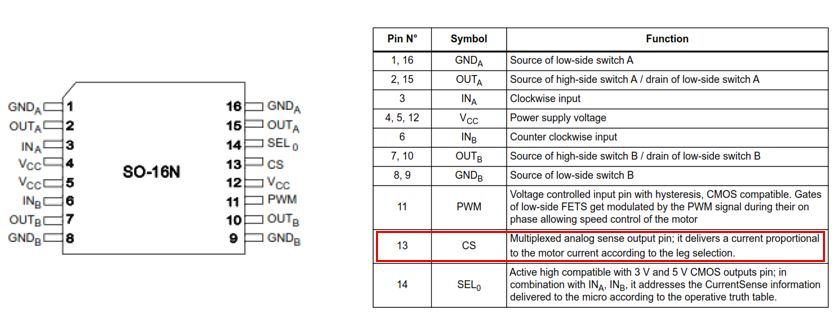
\includegraphics[width=2.5cm]{CHPTRS/CH04_DIS_ELECTRONICO/Fig_Componentes/DIS_ELEC_06_DriverVNH.jpg} VNH7070BAS
          & 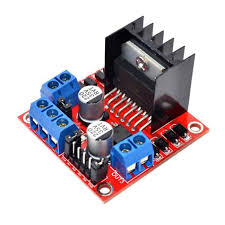
\includegraphics[width=2.5cm]{CHPTRS/CH04_DIS_ELECTRONICO/Componentes/L298N.jpeg} L298N
          & 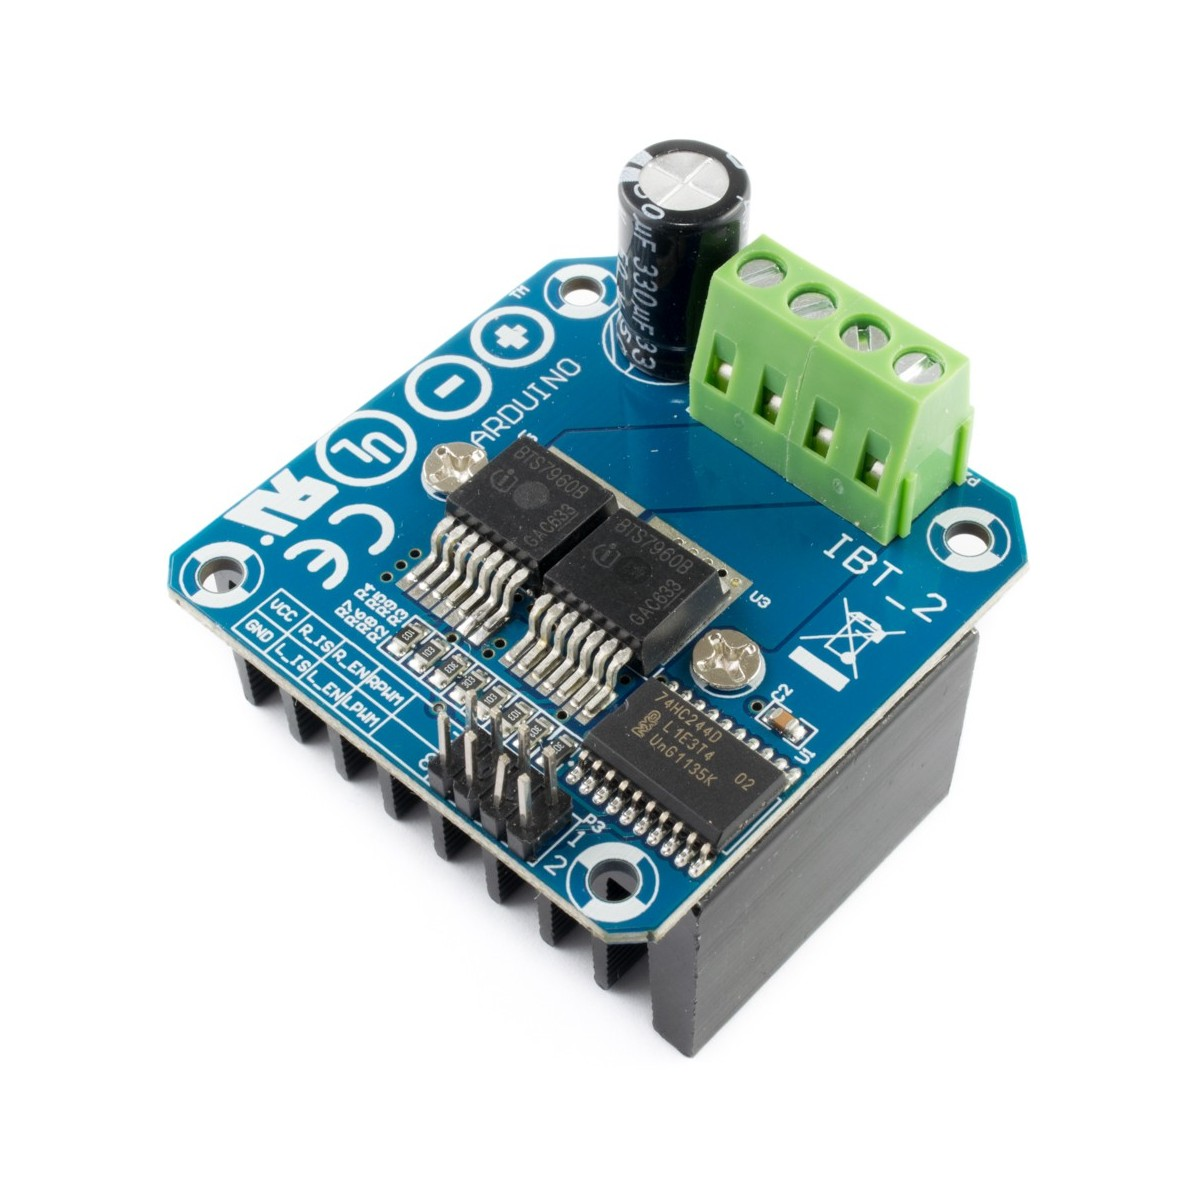
\includegraphics[width=2.5cm]{CHPTRS/CH04_DIS_ELECTRONICO/Fig_Componentes/DIS_ELEC_04B_DriverBTS7960.jpg} BTS7960\\
            Topología
              & Puente H completo integrado (4 MOSFET de potencia)
              & Doble puente H con transistores bipolares (BJT)
              & Medio puente (se requieren \emph{dos} para formar un puente H) \\
            Tecnología de potencia
              & MOSFET automotriz (VIPower M0-7)
              & Transistores BJT de potencia
              & MOSFET (NovalithIC: P-canal alta, N-canal baja) \\
            Alimentación típica
              & \(V_{\mathrm{CC}}\) de 4--28\,V
              & Hasta 46\,V (lógica a 5\,V)
              & Operativo 5.5--27.5\,V \\
            Entradas lógicas
              & Umbrales CMOS (\(V_{\mathrm{IH}}\sim 2.1\,\mathrm{V}\), \(V_{\mathrm{IL}}\sim 0.9\,\mathrm{V}\)); compatible 3.3\,V
              & TTL; lógica a 5\,V (\(V_{\mathrm{IH}}\ge 2.3\,\mathrm{V}\))
              & TTL/CMOS; pines IN/INH \\
            PWM
              & Entrada PWM  (frecuencia máxima de 20 kHz)
              & Soporta conmutación, pero con pérdidas elevadas por BJT
              & PWM hasta (frecuencia máxima de 25  kHz) \\
            Sensado de corriente
              & Sí, pin CS brinda una corriente proporcional a la del motor
              & Pines “Sense” para resistores externos; \emph{no} hay espejo/ganancia integrada
              & Sí, pin IS brinda corriente proporcional a la del motor  \\
            Protecciones
              & Sobre-corriente, sobre-temperatura y protección sobre-corriente en caso de cortocircuito
              & Sobre-temperatura
              & \textit{Current limit} (\(\approx \SI{43}{A}\)), sobre-temperatura; \emph{dead-time} interno \\
            Integración / BOM
              & Un solo CI para un motor bidireccional $+$ sensado
              & Un solo CI, pero con diodos externos y pérdidas altas
              & Dos CI para un puente H completo (uno por rama) \\
       \end{longtblr}
       \begin{figure}[H]
            \centering
            \begin{tabularx}{\linewidth}{>{\centering\arraybackslash}X}
                % Fila 1: imagen
                \begin{subfigure}[t]{\linewidth}
                    \centering
                    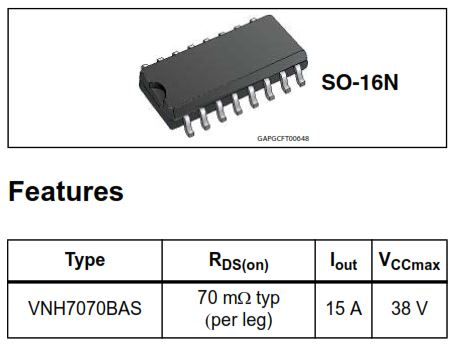
\includegraphics[width=0.5\linewidth]{CHPTRS/CH04_DIS_ELECTRONICO/Fig_Componentes/DIS_ELEC_05_DriverVNH.jpg}
                \end{subfigure}
            \end{tabularx}
            \caption{Integrado CH340 cargar el programa y de poder comunicarse con el micrcontrolador elegido}
            \label{fig:black_box}
        \end{figure}
    \subsection{Selección de sensor de corriente}
        Se adopta el sensado de corriente integrado del puente H VNH7070BAS, el cual presenta en el pin CS una señal proporcional a la corriente del motor. Esta elección elimina la necesidad de un sensor de corriente \ac{DC} adicional y reduce complejidad y ocupación en la \ac{PCB}.         
        En la sección \ref{sec:diseño_driver} se diseña un pequeño circuito de adecuación para que la señal de CS sea compatible con el ADC del microcontrolador (\SI{0}{\volt}–\SI{3.3}{\volt})
        \begin{figure}[H]
            \centering
            \begin{tabularx}{\linewidth}{>{\centering\arraybackslash}X}
                % Fila 1: imagen
                \begin{subfigure}[t]{\linewidth}
                    \centering
                    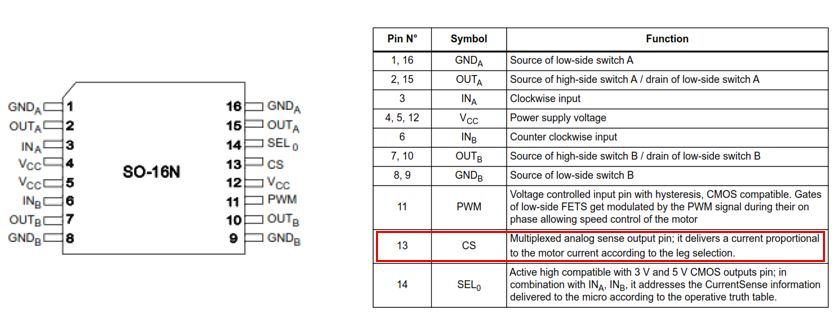
\includegraphics[width=0.75\linewidth]{CHPTRS/CH04_DIS_ELECTRONICO/Fig_Componentes/DIS_ELEC_06_DriverVNH.jpg}
                \end{subfigure}
            \end{tabularx}
            \caption{Integrado CH340 cargar el programa y de poder comunicarse con el micrcontrolador elegido}
            \label{fig:black_box}
        \end{figure}
        Finalmente, en el capítulo de implementación se calibrará la ganancia real del sensado (\(K_{\text{CS}}\)) y su posible offset mediante ensayos comparativos con un sensor de corriente de referencia. Con dichos datos se ajustará el modelo de conversión a la forma
        \[
        I_{\text{motor}} = \alpha\,V_{\text{ADC}} + \beta,
        \]
        dejando documentados \(\alpha\) (ganancia efectiva) y \(\beta\) (offset) para mejorar la exactitud de las mediciones en las pruebas del prototipo.

    \subsection{Selección de fuente de alimentación}

        Dado el requisito de conexión directa a red (\SI{220}{\volt}–\SI{60}{\hertz}), se seleccionó una \ac{SMPS} en lugar de una fuente lineal. Las \ac{SMPS} ofrecen mayor eficiencia y densidad de potencia, reduciendo volumen y masa al prescindir del transformador de \SI{60}{\hertz} propio de las topologías lineales; estas características favorecen la integración del sistema en un chasis compacto (véase \cite{fswitchignfuentelineal}). 
        \begin{figure}[H]
            \centering
            \begin{tabularx}{\linewidth}{>{\centering\arraybackslash}X}
                % Fila 1: imagen
                \begin{subfigure}[t]{\linewidth}
                    \centering
                    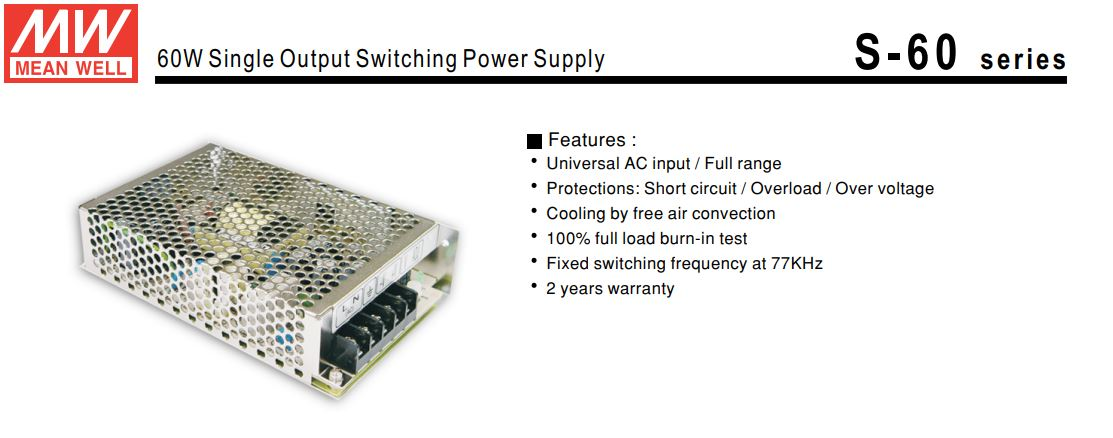
\includegraphics[width=0.5\linewidth]{CHPTRS/CH04_DIS_ELECTRONICO/Fig_Componentes/DIS_ELEC_07_FuenteSwitching.jpg}
                \end{subfigure}
            \end{tabularx}
            \caption{Fuente \textit{switching} elegida para alimentar la \ac{PCB} de control}
            \label{fig:smps}
        \end{figure}
        En particular, se empleará la MEAN WELL serie S-60 mopstrada en la Figura \ref{fig:smps}, con entrada universal \SI{85}{\volt}–\SI{264}{\volt}~\ac{AC} y protecciones contra cortocircuito, sobrecarga y sobretensión, por lo que no es necesario diseñar desde cero la etapa \ac{AC}/\ac{DC}. El modelo específico es el S-60-12 se selecciona según la tensión y potencia requeridas por los módulos del sistema, manteniendo margen de diseño.
\section{Diseño de \ac{PCB}}
    En esta sección se diseñan los circuitos necesarios para la implementación del banco de pruebas, los cuales se estructuran en coherencia con los dominios definidos en el Capítulo \ref{ch:CH03-Diseno-Conceptual}. En particular, se aborda: (i) la etapa de regulación de voltaje para la alimentación distribuida de los módulos, (ii) la electrónica de control empleada durante la caracterización del motor, (iii) la interfaz de comunicación con el \ac{SW}, y (iv) el acondicionamiento y la adquisición de señales de los sensores necesarios para la extracción de datos del motor.
    \subsection{Diseño de circuitos de potencia}
        Para energizar todo el sistema de control se requiere regular el voltaje que entrega la fuente \textit{switching}, la cual proporciona \SI{12}{\volt} \ac{DC}. Dado que el microcontrolador ESP32, el sensor y el módulo Ethernet operan a \SI{3.3}{\volt}, se empleará una fuente \ac{DC}-\ac{DC} de topología \textit{buck}. Como se muestra en la Figura \ref{fig:RegDeVoltaje}, se utiliza el regulador LM2594 junto con los componentes propios de una fuente \textit{buck}.
        \begin{figure}[H]
           \centering
           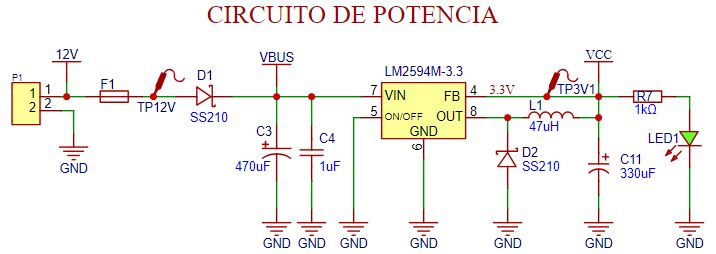
\includegraphics[width=1\textwidth]{CHPTRS/CH04_DIS_ELECTRONICO/Fig_Esquematicos/DIS_ELEC_01_CircuitoDePotencia.jpg}
           \caption{Diagrama esquemático del regulador de voltaje de la \ac{PCB} de control}
           \label{fig:RegDeVoltaje}
        \end{figure}
        Los valores de los capacitores y bobinas que acompañan al integrado LM2594 son provistos y ya están calculados por el fabricante, como se muestra en la Figura \ref{fig:CircuitoDeRegulacion}. Además de estos componentes, en la Figura \ref{fig:RegDeVoltaje} se incluye un fusible para proteger ante sobrecorrientes toda la \ac{PCB} de control, así como un LED indicador del estado de energización del sistema.
        \begin{figure}[H]
           \centering
           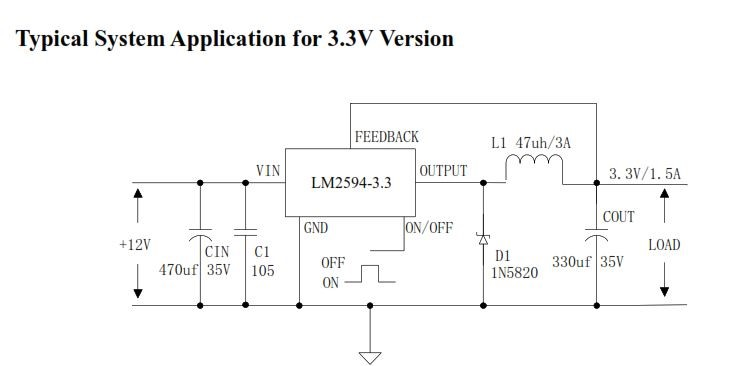
\includegraphics[width=1\textwidth]{CHPTRS/CH04_DIS_ELECTRONICO/Fig_Esquematicos/DIS_ELEC_01_CircuitoDePotenciaRecomendado.jpg}
           \caption{Diseño típico de regulador LM2594}
           \label{fig:CircuitoDeRegulacion}
        \end{figure}
    \subsection{Diseño de circuitos de control}
        Para la parte de control se utilizará el chip de la ESP32-32D, donde el primer paso es investigar sobre su distribución de pines y características de su \textit{datasheet}. Para ello, en la Figura \ref{fig:PinesESP32} se muestra la distribución de pines y las funciones que estos cumplen como se detalla a continuación:
        \begin{itemize}
          \item Pines digitales: entradas/salidas lógicas (0/1), con posibilidad de interrupciones y \textit{pull-up}/\textit{pull-down} configurables.
          \item Pines analógicos: lectura de señales continuas mediante ADC de 12 bits, convirtiéndolas en valores digitales procesables.
          \item Pines PWM: generación de señales con ciclo útil variable para controlar velocidad de motores o intensidad de LEDs.
          \item Pines de alimentación: VCC (3.3\,V) y GND, indispensables para el funcionamiento del módulo.
          \item Pines de comunicación: interfaces UART (TX/RX), SPI (MOSI/MISO/SCK/CS) e I\textsuperscript{2}C (SDA/SCL) para intercambio de datos con periféricos.
        \end{itemize}
        \begin{figure}[H]
            \centering
            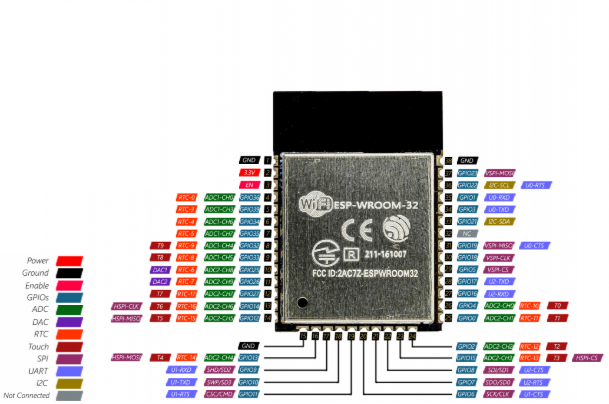
\includegraphics[width=0.7\textwidth]{CHPTRS/CH04_DIS_ELECTRONICO/Fig_Pinout/PINOUT_01_ESP32.png}
            \caption{Pinout del microcontrolador ESP32}
            \label{fig:PinesESP32}
        \end{figure}
        Para esta aplicación se empleará un único bus SPI compartido entre la ESP32, el sensor TMAG7051 y el módulo Ethernet ENC28J60 (véase el Anexo \ref{an:Anexo_J_ComunicacionSPI}). Se asignan GPIO18 como SCK, GPIO23 como MOSI y GPIO19 como MISO; y líneas de selección independientes: GPIO5 como CS del TMAG7051 y GPIO22 como CS del ENC28J60. Opcionalmente, el pin INT del ENC28J60 puede conectarse al GPIO27 para notificación de eventos. Todos los módulos operan a 3.3,V y comparten una tierra común. Estas conexiones se muestran en la Figura \ref{fig:DiagramaConexiones}, correspondiente al esquema de la \ac{PCB} de control.
        \begin{figure}[H]
            \centering
            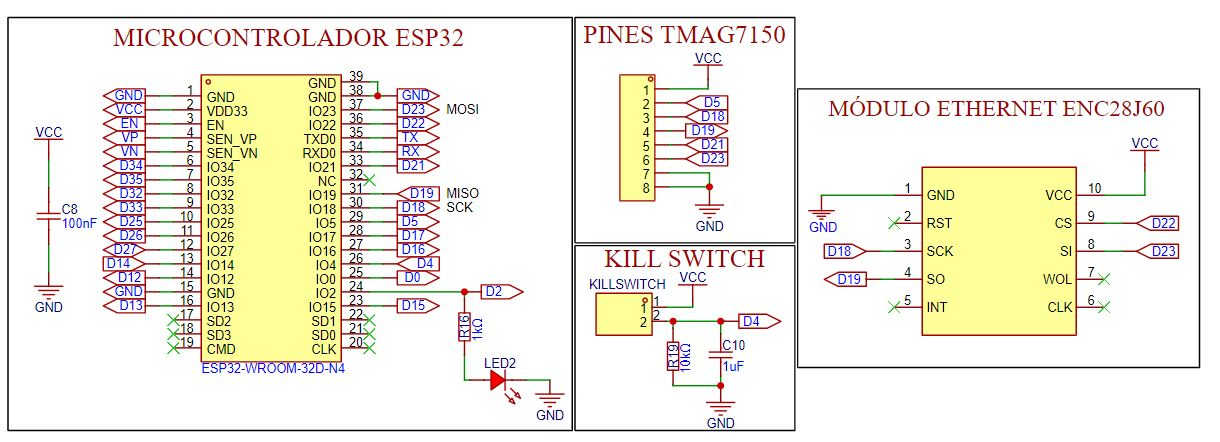
\includegraphics[width=1\textwidth]{CHPTRS/CH04_DIS_ELECTRONICO/Fig_Esquematicos/DIS_ELEC_04_CircuitoDeConexiones.jpg}
            \caption{Diagrama de conexiones entre el microcontrolador, módulo de Ethernet y sensor de efecto \textit{hall} TMAG5170}
            \label{fig:DiagramaConexiones}
        \end{figure}
    \subsection{Diseño de circuito para VNH7070BAS}
    \label{sec:diseño_driver}
        Para controlar el puente H se emplearán pines de la ESP32 para el ciclo de trabajo, la habilitación de sentidos de giro y la medición de corriente. El integrado requiere dos referencias unidas en un punto estrella: tierra de señal (microcontrolador, GPIO y \ac{PWM}) y tierra de potencia de la fuente del motor.
        \begin{figure}[H]
            \centering
            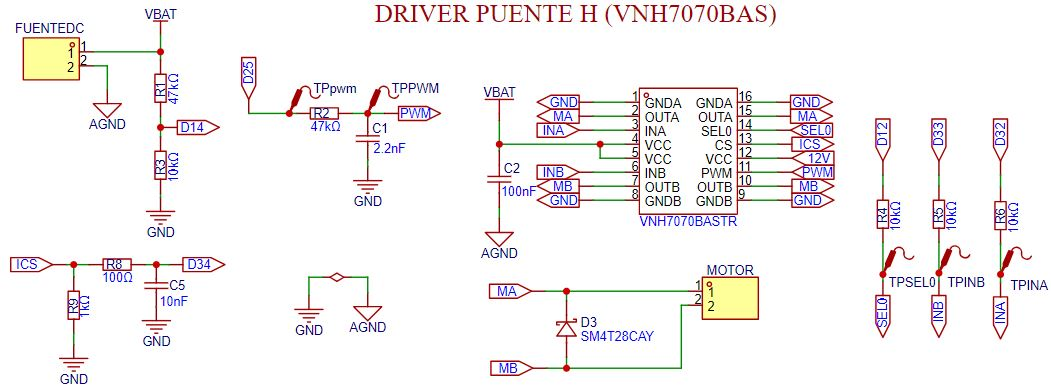
\includegraphics[width=1\textwidth]{CHPTRS/CH04_DIS_ELECTRONICO/Fig_Esquematicos/DIS_ELEC_03_CircuitoDeDriverPuenteH.jpg}
            \caption{Diagrama esquemático de conexiones con el driver VNH7070BAS}
            \label{fig:DiagramaConexiones}
        \end{figure}
        VBAT recibe el voltaje nominal del motor. Se coloca un condensador cerámico de \SI{100}{\nano\farad} lo más próximo posible a VBAT–AGND y, en la entrada, un condensador electrolítico (\SI{47}{\micro\farad}–\SI{220}{\micro\farad}) para amortiguar el transitorio. La alimentación lógica VCC (3,3–5V) lleva su propio \SI{100}{\nano\farad} junto a los pines del CI. Dado que no tolera polaridad inversa, se recomienda protección de entrada (MOSFET de protección o diodo serie) según la caída de tensión admisible.
        
        El TVS SM4T28CAY se conecta entre MA y MB el cual sirve como un diod de protección que se conecta en paralelo al motor para disipar las corrientes que almacene el motor luego de su uso, para que estas no se devuelvan al driver y que mas bien se consuman con el diodo.
        
        INA, INB, \ac{PWM} y SEL0 se conectan a GPIO de la ESP32 con resistencias \textit{pull-down} de \SI{10}{\kilo\ohm} para evitar estados flotantes al arranque. La \ac{PWM} opera típicamente entre 10–20 kHz; si es necesario mitigar EMI, se limita el \textit{slew rate} con una red RC pequeña cerca del pin . Evitar redes que promedien la \ac{PWM}, pues distorsionan el ciclo efectivo en una entrada digital.
        
        El pin CS entrega una corriente proporcional a la corriente de fase \(I_{\text{OUT}}\) con factor \(K_{\text{ILIS}}\). Se convierte a tensión con una resistencia \(R_{\text{CS}}\) a GND y se filtra con un condensador (R8 y C5 como filtro \textit{anti-aliasing}):
        \[
        V_{\text{CS}} = I_{\text{OUT}}\cdot K_{\text{ILIS}}\cdot R_{\text{CS}}.
        \]
        Al dimensionar \(R_{\text{CS}}\), garantizar \(V_{\text{CS}}\leq V_{\text{ADC,max}}\) (\SI{3.3}{\volt}) para la corriente máxima y respetar el límite del pin CS (\(\leq\) 10 mA \ac{DC}). Para precisión, el retorno de CS y el GND del ADC deben ir por conexión Kelvin al punto estrella.
        
        Los bornes del motor se conectan a MA/MB. El bucle de alta corriente (Vbat hacia el motor) debe ser lo más corto y compacto posible; en PCB, usar plano de potencia, \textit{vias} térmicas bajo el CI y anchos de pista acordes a la corriente. Durante el arranque, establecer un estado seguro: INA = INB = 0 y \ac{PWM} = 0 hasta completar la inicialización.
        
        El VNH7070BAS integra limitación de corriente, protección de cortocircuito y \textit{thermal shutdown} con \textit{auto-retry}. Son funciones de protección y no sustituyen el control de corriente de la aplicación; para un límite programable se cierra un lazo digital leyendo CS y modulando la \ac{PWM} en \textit{firmware}.

    
    \subsection{Diseño de circuitos para el sensor de efecto \textit{hall} TMAG5170}
        La placa integra el sensor TMAG5170 y lo conecta con la placa principal (ESP32) mediante un conector de ocho vías. La alimentación es de 3.3 V y se comparte la referencia de masa con la placa principal. El acondicionamiento local incluye dos condensadores de desacoplo próximos entre VCC y GND del CI: C8 = 100 nF (alta frecuencia) y C2 = 1 µF (baja impedancia a media y baja frecuencia). La interfaz SPI se enruta en cuatro hilos (SCK, SDI/MOSI, SDO/MISO y CS); para mejorar la integridad de señal se añade una resistencia en serie R4 = 100 ohm en SCK, colocada cerca del TMAG5170, que atenúa los flancos y reduce el “ringing” sin afectar el temporizado. El pin ALERT, de tipo drenador abierto, se eleva con un pull-up R5 = 4.7 kohm a 3.3 V para indicar “data-ready” o diagnóstico hacia el microcontrolador. El pin TEST se fija a GND según la recomendación del fabricante. Todas las señales operan a niveles CMOS de 3.3 V; se recomienda mantener las pistas del bus cortas, con retorno de masa directo bajo cada traza y alejadas del lazo de potencia del puente H. Mecánicamente, para la medición on-axis (imán diametral coaxial al encapsulado), la placa debe alinearse de modo que el centro del imán coincida con el centro del CI y con holgura axial estable; esta orientación permite estimar el ángulo en el plano XY con mínima elipticidad. La lectura angular puede obtenerse directamente del TMAG5170 o calcularse en la ESP32 a partir de Bx y By mediante la función atan2(By, Bx).

        \begin{figure}[H]
           \centering
           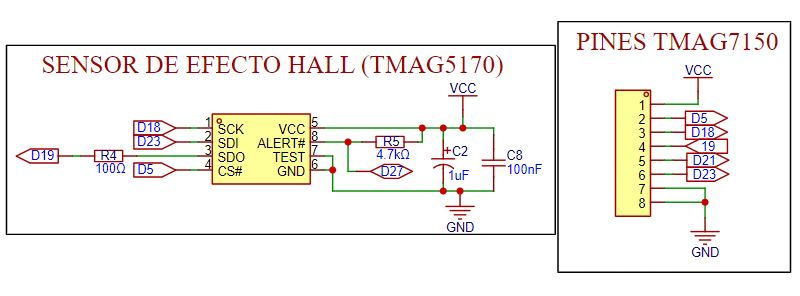
\includegraphics[width=1\textwidth]{CHPTRS/CH04_DIS_ELECTRONICO/Fig_Esquematicos/DIS_ELEC_05_CircuitoDeSensorTMAG7150.jpg}
           \caption{Diagrama esquemático con las conexiones del sensor de efecto \textit{hall}}
           \label{fig:switching}
        \end{figure}
        
        \medskip
        Configuración por registros (resumen). La programación detallada se desarrollará en el Capítulo de Pruebas de Prototipo; de forma resumida se configurarán:
        \begin{itemize}
          \item SENSOR\_CONFIG: habilitar X e Y, seleccionar el \textit{full-scale} por eje (por ejemplo, \(\pm 25/\pm 50/\pm 100\,\text{mT}\) en A1) y activar el cálculo de ángulo en \(XY\).
          \item DEVICE\_CONFIG y/o SYSTEM\_CONFIG: elegir el modo de conversión (continuo o por disparo), el promediado/\textit{oversampling} y, si aplica, el filtro digital para mejorar la relación señal–ruido.
          \item ALERT\_CONFIG: configurar ALERT como \textit{data-ready} para sincronizar la lectura desde la ESP32.
          \item Lectura periódica de ANGLE\_RESULT (o de BX/BY para cálculo con \(\operatorname{atan2}\)) y calibración de offset de cero.
        \end{itemize}

    \subsection{Diseño de circuitos de comunicación}
        El circuito implementa un puente USB–UART con el CH340 y un conector USB-C configurado como dispositivo mediante resistencias de 5.1 kohm en CC1/CC2; las líneas D+ y D$-$ se enrutan al CH340 con desacoplo local. El CH340 convierte los datos del PC a UART y enlaza TXD con RX0 y RXD con TX0 de la ESP32. Para el autoprogramado, las salidas DTR y RTS del CH340, a través de las redes R12/R15 y los transistores Q1/Q2 (con R11/R18 como limitadoras), fuerzan la secuencia de arranque: EN baja/alta mientras IO0 se mantiene bajo, entrando en modo bootloader; luego ambas retornan a alto por las pull-up R10 y R17 y el micro arranca en modo normal. Se incluyen pulsadores BOOT (IO0–GND) y RST (EN–GND) para control manual. Todas las masas comparten GND, y VBUS del conector alimenta la etapa mediante el regulador de la placa.
        \begin{figure}[H]
           \centering
           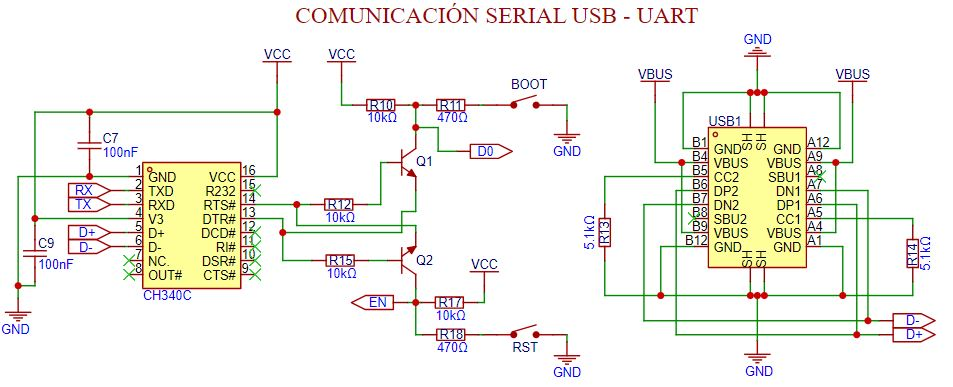
\includegraphics[width=1\textwidth]{CHPTRS/CH04_DIS_ELECTRONICO/Fig_Esquematicos/DIS_ELEC_02_CircuitoDeComunicacionPC.jpg}
           \caption{Diagrama esquemático del circuito de comunicación USB-UART}
           \label{fig:switching}
        \end{figure}
Finalmente, en la Tabla \ref{tab:pines_pcb} se presenta la distribución de pines del microcontrolador, con el fin de visualizar qué pines se utilizarán y configurar cada uno según su función en el programa que se cargará en la ESP32.

\begin{table}[H]
    \centering
    \caption{Pines utilizados en la PCB}
    \begin{tabularx}{0.92\textwidth}{l l X}
    \toprule
    Pin & Configuración & Función \\
    \midrule
    GPIO2  & GPIO (salida)          & LED ROJO \\
    GPIO4  & GPIO (entrada/INT)     & Interrupción (kill switch) \\
    GPIO5  & SPI (CS)               & CS SENSOR \\
    GPIO12 & GPIO (salida)          & SEL0 \\
    GPIO14 & ADC (entrada)          & ADC (MEDIR VOLTAJE de batería) \\
    GPIO18 & SPI (SCK)              & SCK \\
    GPIO19 & SPI (MISO)             & MISO \\
    GPIO22 & SPI (CS)               & CS PUERTO ETHERNET \\
    GPIO23 & SPI (MOSI)             & MOSI \\
    GPIO25 & PWM (LEDC)             & PWM driver \\
    GPIO27 & GPIO (entrada)         & STATUS OUTPUT TRIGERED \\
    IO32   & GPIO (salida)          & INA \\
    IO33   & GPIO (salida)          & INB \\
    GPIO34 & ADC (entrada)          & ADC (MEDIR CORRIENTE) \\
    \midrule
    TX     & UART (TX0)             & SUBIDA DE PROGRAMA \\
    RX     & UART (RX0)             & SUBIDA DE PROGRAMA \\
    D0     & BOOT           & SUBIDA DE PROGRAMA \\
    EN     & EN      & SUBIDA DE PROGRAMA \\
    \bottomrule
    \end{tabularx}
    \label{tab:pines_pcb}
\end{table}

% \section{Diseño de protocolo de comunicación con la interfaz con módulo Ethernet}

%     \begin{figure}[H]
%        \centering
%        \includegraphics[width=0.4\textwidth]{ethe}
%        \caption{\ac{PCB} de una fuente \textit{switching}}
%        \label{fig:switching}
%     \end{figure}
\section{Diagramas electrónicos}
    En esta sección se presenta el diagrama de conexiones entre la \ac{PCB} de control y la \ac{PCB} del sensor de efecto \textit{hall}. La Figura \ref{fig:pcb_control_full} muestra el esquema de la \ac{PCB} de control, mientras que la Figura \ref{fig:pcb_sensor_full} corresponde a la placa de adaptación del TMAG5170. En la sección siguiente se detallan los criterios de ruteo y el diseño final para su ensamble en el chasis.
    
    % Página 1 (figura rotada con leyenda rotada)
    \begin{sidewaysfigure}
      \centering
      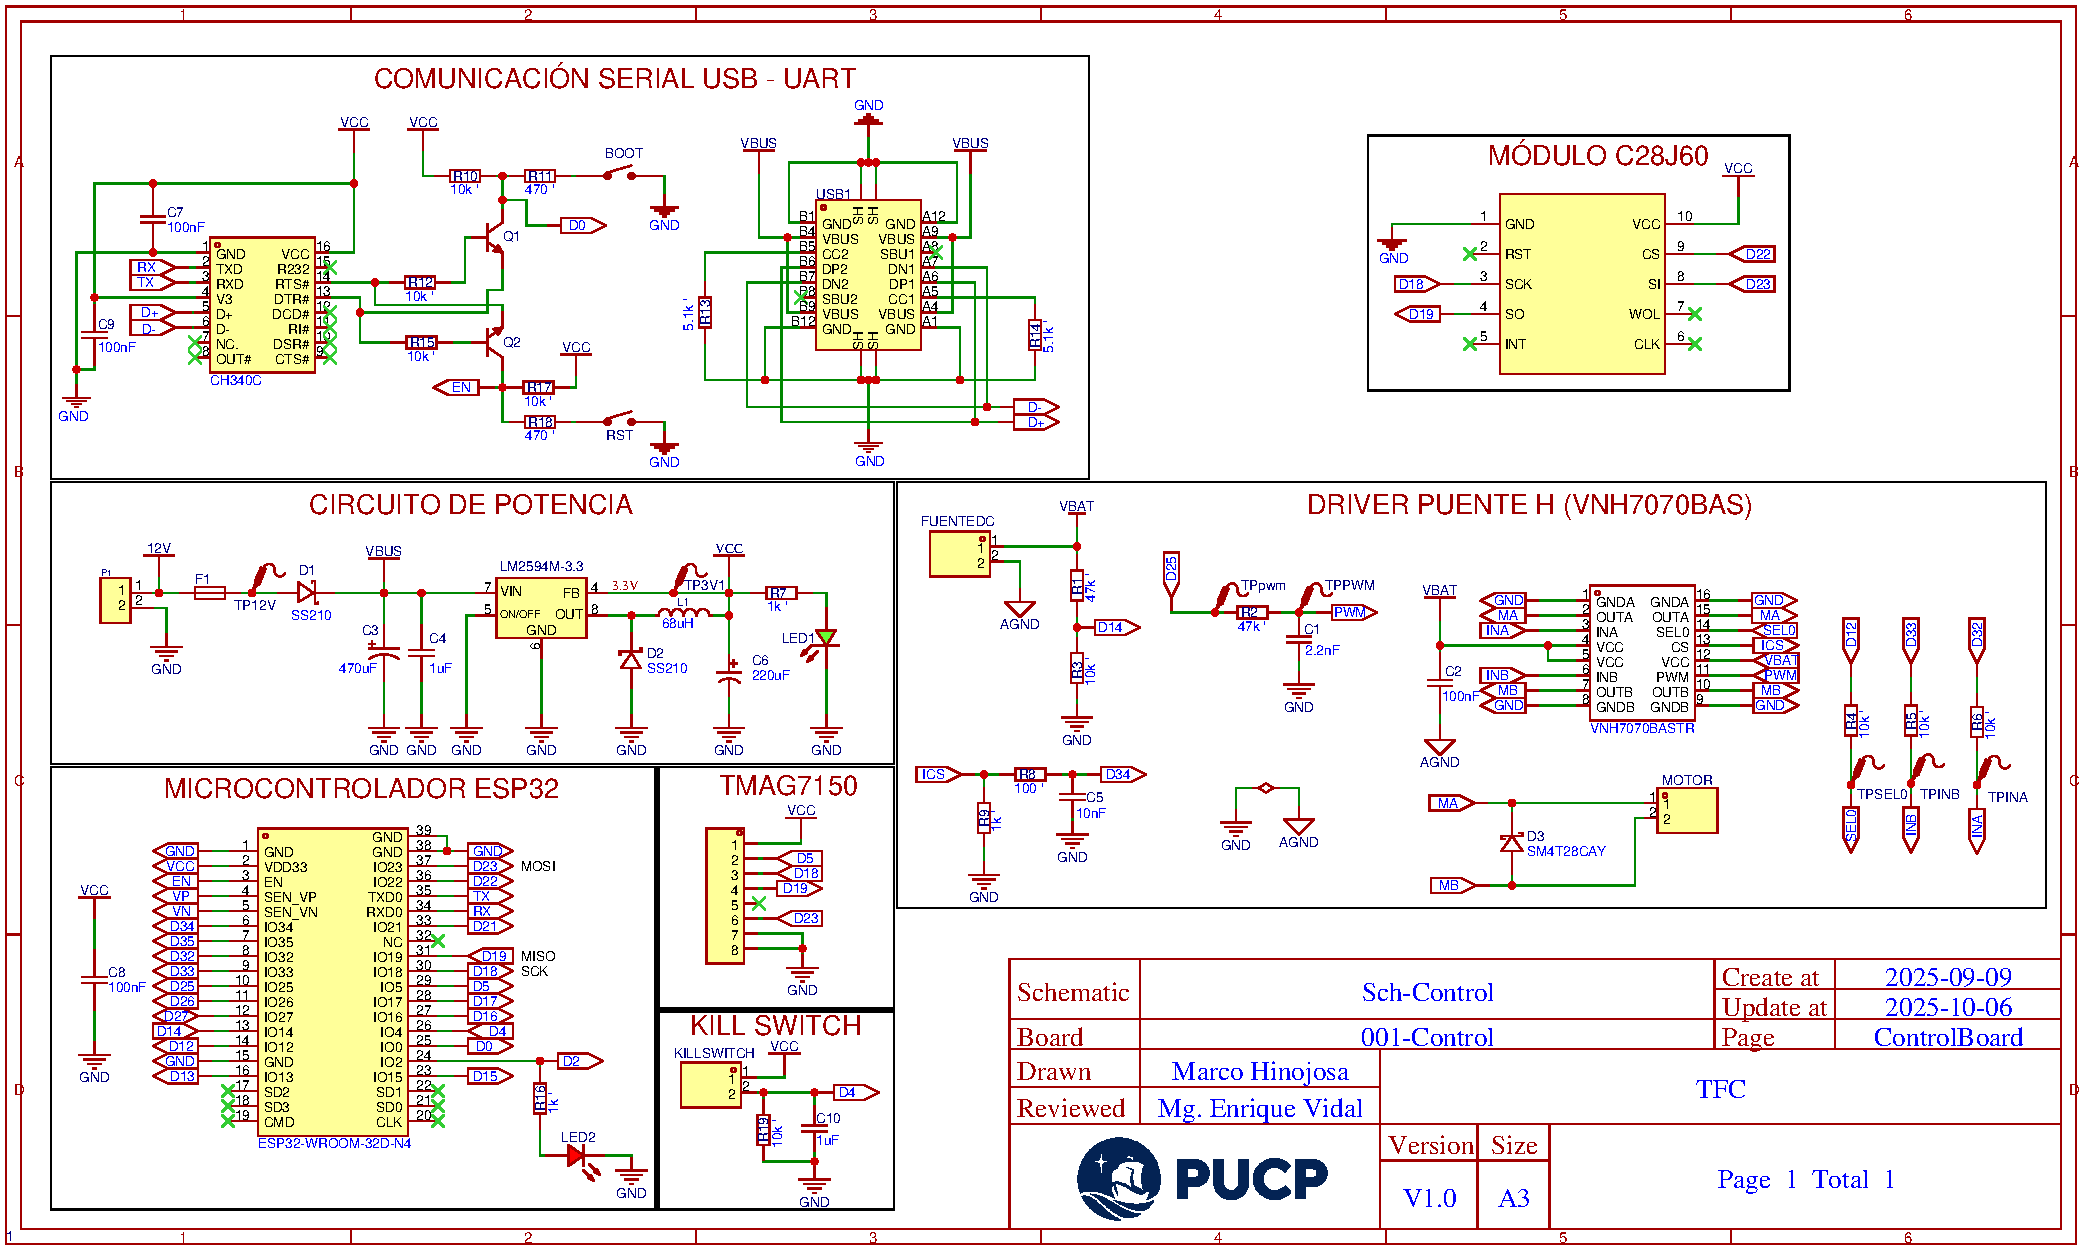
\includegraphics[width=\textheight]{CHPTRS/CH04_DIS_ELECTRONICO/Fig_Esquematicos/DIS_ELEC_06_DiagramaEsquematico.pdf}
      \caption{Diagrama esquemático general para la \ac{PCB} de control}
      \label{fig:pcb_control_full}
    \end{sidewaysfigure}
    
    % Página 2 (figura rotada con leyenda rotada)
    \begin{sidewaysfigure}
      \centering
      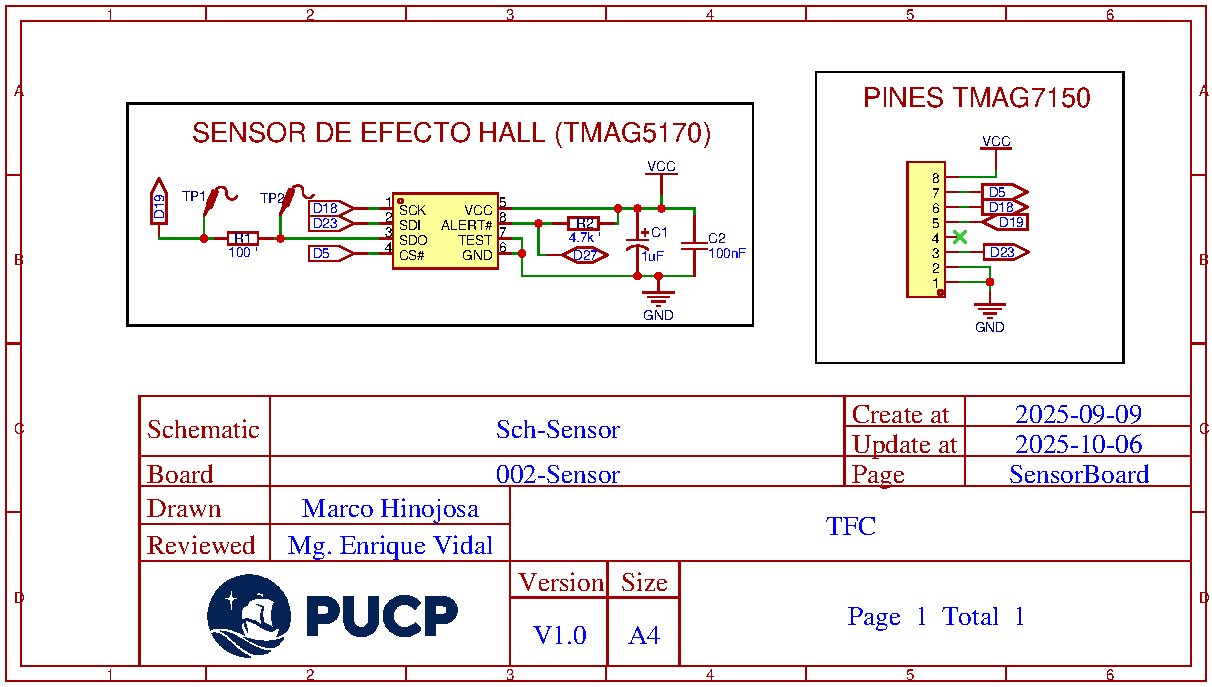
\includegraphics[width=\textheight]{CHPTRS/CH04_DIS_ELECTRONICO/Fig_Esquematicos/DIS_ELEC_07_DiagramaEsquematicoSensor.pdf}
      \caption{Diagrama esquemático con las conexiones del sensor de efecto \textit{hall}}
      \label{fig:pcb_sensor_full}
    \end{sidewaysfigure}

\section{Diseño de las \ac{PCB}s}
    Con base en lo anterior, se procede al ruteo de la \ac{PCB}. Se aplican las recomendaciones del fabricante y los criterios de integridad térmica y eléctrica. En particular, para el VNH7070BAS se siguen las pautas de disipación y almohadillas térmicas mostradas en la Figura \ref{fig:layerVNH7070BAS}.

    \begin{figure}[H]
       \centering
       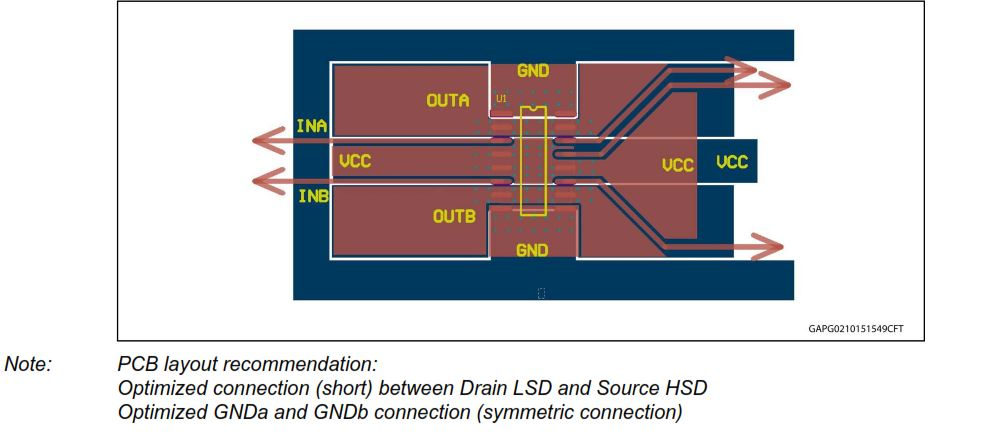
\includegraphics[width=0.8\textwidth]{CHPTRS/CH04_DIS_ELECTRONICO/Fig_DiseñoPCB/LayerVNH7070BAS.JPG}
       \caption{Recomendación del fabricante respecto a las \textit{layers} superficies de disipación y trazas del driver VNH7070BAS}
       \label{fig:layerVNH7070BAS}
    \end{figure}
    
    Asimismo, se define la ubicación de conectores y la distribución de componentes en el chasis, priorizando recorridos de cable cortos, accesibilidad a alimentación, comunicación y mandos, y evitando cruces. La Figura \ref{fig:Distribución de componentes} presenta un esquema con una vista superior con las salidas hacia la \ac{PCB} y la ubicación de los elementos del chasis.
    
    \begin{figure}[H]
       \centering
       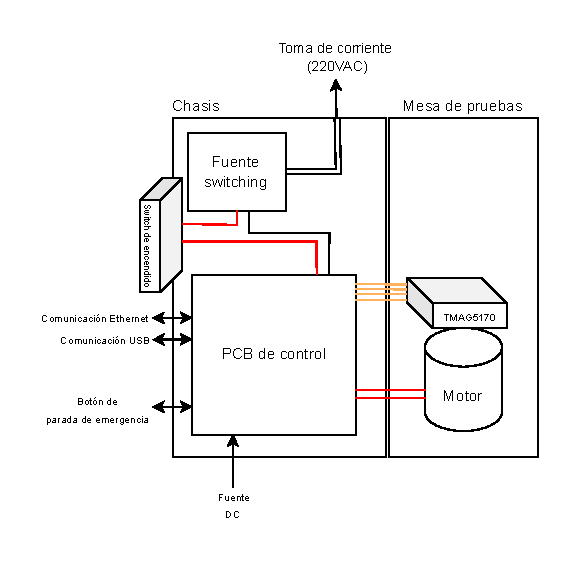
\includegraphics[width=0.8\textwidth]{CHPTRS/CH04_DIS_ELECTRONICO/Fig_Esquematicos/DistribuciónDeComponentes.pdf}
       \caption{Distribución de componentes y conectores (vista superior)}
       \label{fig:Distribución de componentes}
    \end{figure}
    
    El ancho de pista se dimensiona con el modelo IPC-2221. Para una corriente \(I\) y un aumento de temperatura objetivo \(\Delta T\):
    \begin{align*}
      A~[\text{mil}^2] &= \left(\frac{I~[\text{A}]}{k\,(\Delta T~[^\circ\text{C}])^{b}}\right)^{\tfrac{1}{c}},\\
      W~[\text{mil}] &= \frac{A~[\text{mil}^2]}{t_\text{cu}~[\text{mil}]},
    \end{align*}
    Donde, para las capas externas, k = 0.048, b = 0.44, c = 0.725 y el espesor de cobre es 1.378 mil (1 oz por pie cuadrado).\footnote{1 mil equivale a 0,0254 mm; 1 oz por pie cuadrado equivale aproximadamente a 1,37 a 1,378 mil, es decir, cerca de 35 micrómetros.} Para las capas internas se usa k = 0.024 y se mantienen los mismos valores de b y c \cite{DigiKey_TraceWidth}.

    Se considerará un diseño de \ac{PCB} de dos capas con cobre de 1 oz. Asimismo, se asumirá una temperatura ambiente de 25 °C y una elevación térmica de 25 °C.

    \begin{table}[H]\centering
    \caption{Ancho mínimo por corriente (IPC-2221, 1 oz, capa externa, \(\Delta T=25~^\circ\text{C}\)).}
    \begin{tabular}{rcc}
    \toprule
    Corriente & Ancho mínimo [mil] & Ancho mínimo [mm]\\
    \midrule
    0.01 A  & 0.012  & 0.0003 \\
    0.05 A  & 0.109  & 0.0028 \\
    0.10 A  & 0.283  & 0.0072 \\
    0.50 A  & 2.607  & 0.0662 \\
    1.00 A  & 6.781  & 0.1723 \\
    1.50 A  & 11.863 & 0.3013 \\
    2.00 A  & 17.642 & 0.4481 \\
    3.00 A  & 30.862 & 0.7839 \\
    5.00 A  & 62.434 & 1.5858 \\
    \bottomrule
    \end{tabular}
    \end{table}
    
    Notas: (1) Para corrientes pequeñas, el límite lo impone la capacidad de fabricación (por ejemplo, 0.30 mm), no la fórmula. (2) Si se desea menor \(\Delta T\), el ancho requerido aumenta; con 2 oz, el ancho se reduce aproximadamente a la mitad para la misma \(I\).
        
    \subsection*{Criterios prácticos y refuerzos}
        \begin{itemize}
          \item En zonas de potencia de motor, usar polígonos/planos; dejar la pista sin máscara para estañar y aumentar sección cuando sea posible.
          \item Para pasos entre capas en líneas de potencia, colocar múltiples vías en paralelo (via stitching).
          \item Mantener tramos cortos y anchos desde el conector de 12 V hasta el condensador de reserva del driver y desde OUTA/OUTB al bornero del motor; cerrar retornos en un punto estrella de potencia.
        \end{itemize}
    
    \subsection*{Anchos adoptados para esta PCB (1 oz)}
        % Requiere: \usepackage{tabularx,booktabs,array}
    \begin{table}[H]
    \centering
    \caption{Anchos seleccionados por red (consideran mínimo de fábrica y margen térmico).}
    \setlength{\tabcolsep}{5pt}
    \renewcommand{\arraystretch}{1.1}
    \footnotesize
    \begin{tabularx}{0.95\linewidth}{@{}>{\raggedright\arraybackslash}X
                                        >{\raggedright\arraybackslash}l
                                        >{\raggedright\arraybackslash}X@{}}
    \toprule
    \textbf{Red / función} & \textbf{Ancho adoptado} & \textbf{Justificación} \\
    \midrule
    Señales digitales (GPIO, SPI, PWM, ALERT) & 12 mil (0.30 mm) & Mínimo de fábrica; \(I \ll 10\) mA \\
    3.3 V — tramo principal (hasta 1.5 A)     & 24 mil (0.61 mm) & Cálculo 11.86 mil; se duplica por margen \\
    3.3 V — ramales a cargas (ESP32, ENC28J60, TMAG) & 12 mil (0.30 mm) & Corrientes \(\leq\) 0.5 A por ramal; cálculo 2.61 mil \\
    GND (control)                              & Plano            & Menor impedancia y retorno controlado \\
    12 V — entrada (conector → driver)         & 80 mil (2.03 mm) & Margen sobre cálculo 5 A = 62.4 mil; tramo corto y ancho \\
    OUTA/OUTB → bornero motor                  & 100 mil (2.54 mm) + polígono/estañado & Robustez, baja caída; admite picos \\
    Sense y señales analógicas                 & 12 mil (0.30 mm) & Separación de lazos de potencia \\
    \bottomrule
    \end{tabularx}
    \label{tab:anchos_pcb}
    \end{table}

        
        En caso de limitaciones de espacio, priorizar polígonos para potencia y mantener la máscara abierta en los “bus bars” para añadir estaño en el ensamblaje y aumentar la sección.

    
\section{\textit{Layers} de la PCB}
    Este capítulo de diseño electrónico concluye con la presentación de los layers y las vistas \ac{CAD} del diseño de la \ac{PCB} de control y de la \ac{PCB} de sensado de velocidad. Sus dimensiones se tomarán como referencia en el Capítulo \ref{ch:CH04-Diseno-Mecanico}, dedicado al ensamblaje en el chasis. En la Figura \ref{fig:Layers} se muestran las imágenes finales de las tarjetas.
    \begin{figure}[H]
        \begin{tabularx}{\linewidth}{*{2}{>{\centering\arraybackslash}X}}
            % FILA-1, COL-1.
            \begin{subfigure}[t]{0.45\textwidth}
                \centering
                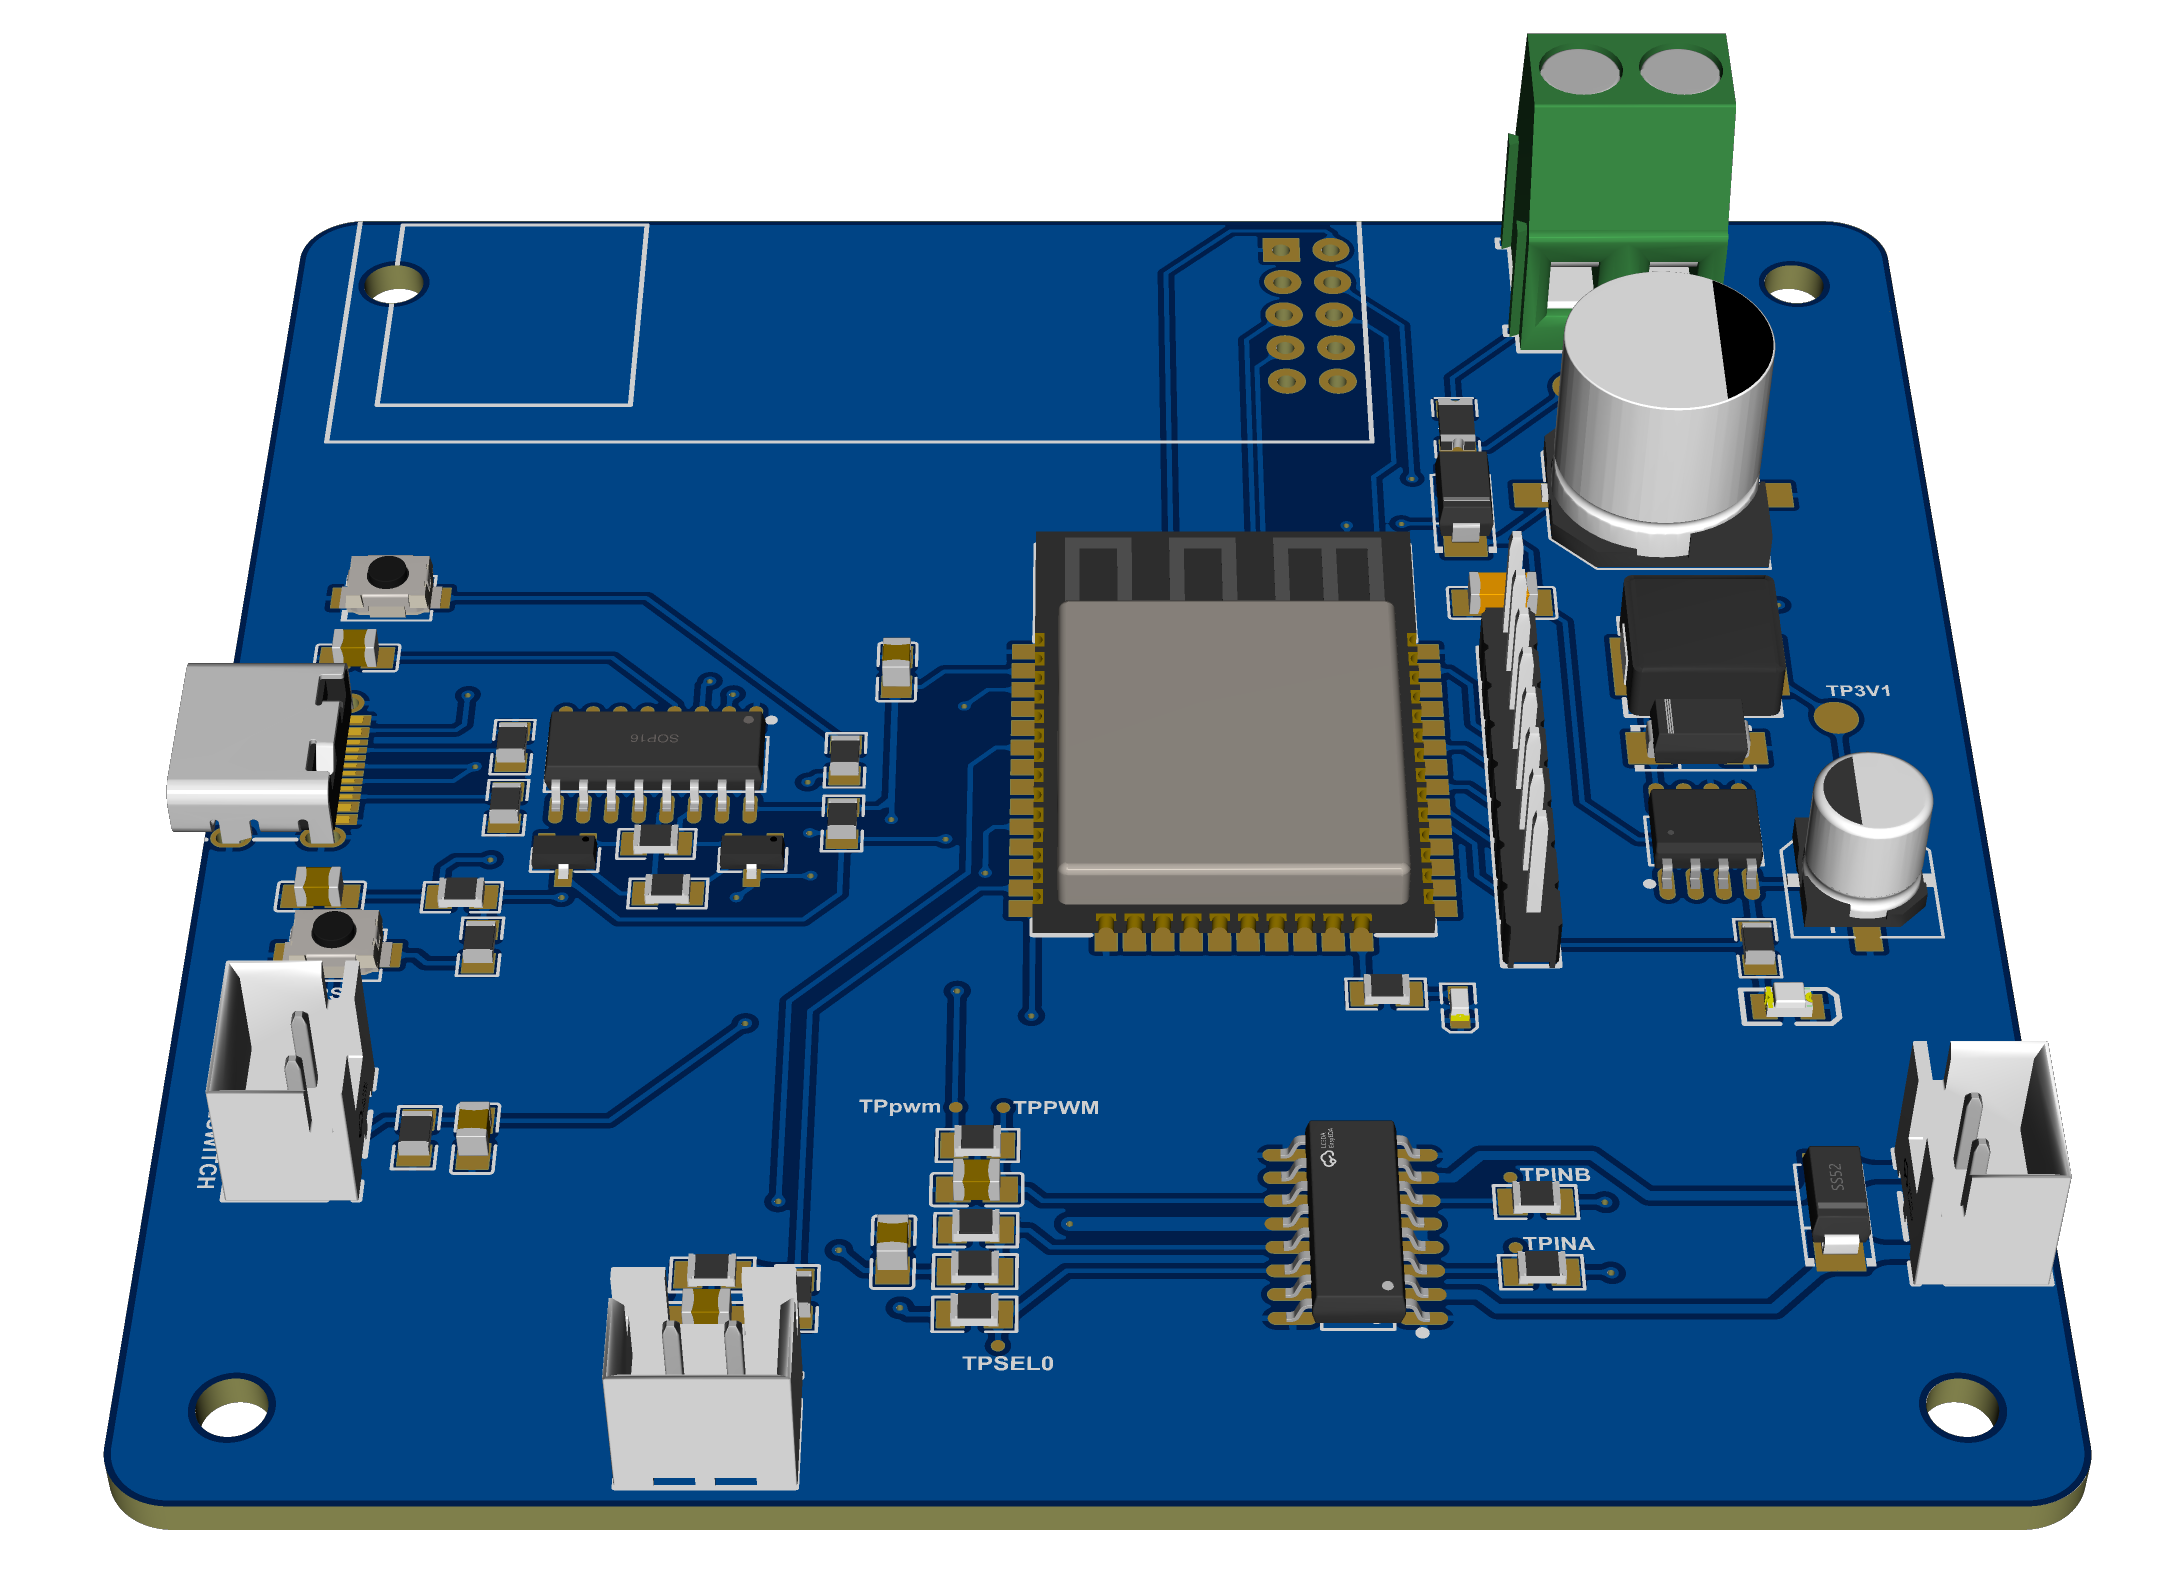
\includegraphics[width=.9\linewidth]{CHPTRS/CH04_DIS_ELECTRONICO/Fig_Esquematicos/PCB_control.png}
                %\label{fig:imagen_pcb_control} %LABEL ESTA DESPUES
            \end{subfigure}
            & %Nueva Columna, es decir: % FILA-1, COL-2
            \begin{subfigure}[t]{0.45\textwidth}
                \centering
                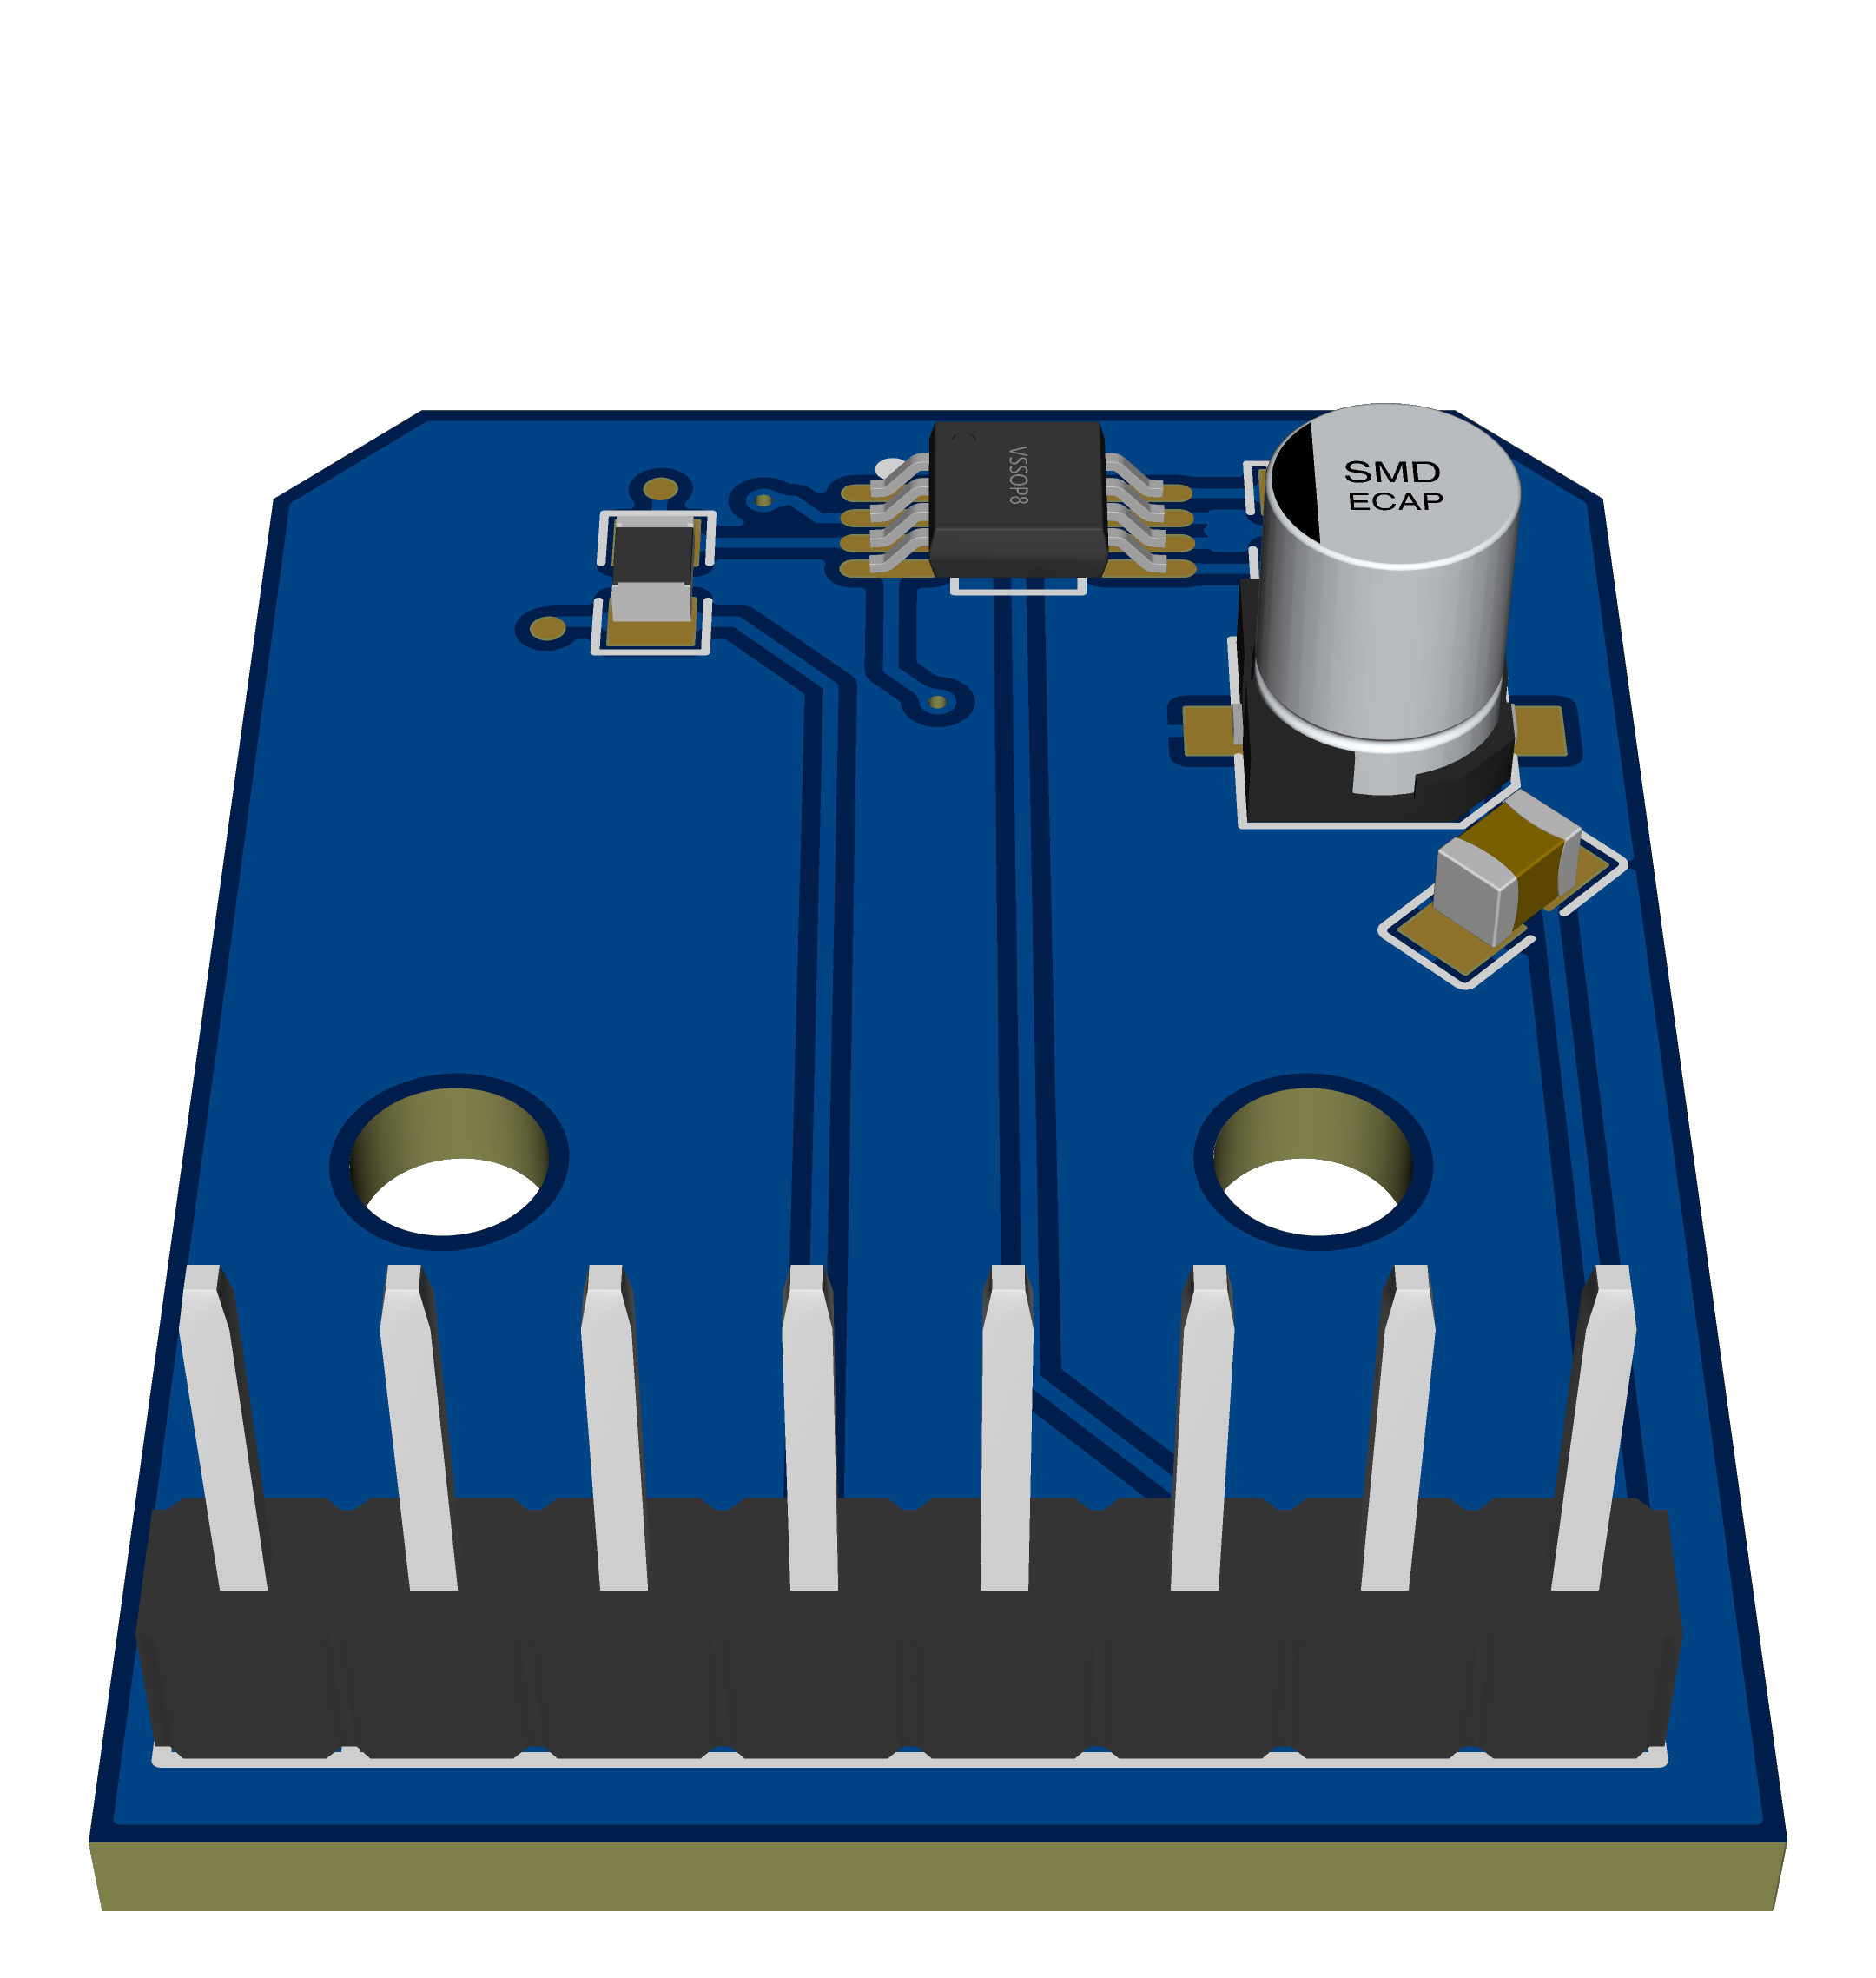
\includegraphics[width=.68\linewidth]{CHPTRS/CH04_DIS_ELECTRONICO/Fig_Esquematicos/PCB_sensor.png}
            \end{subfigure}
            \\ %Nueva Fila, es decir: % FILA-2, COL-1
            \begin{subfigure}[t]{0.8\linewidth}
                \caption{Imagen referencial de cómo quedará la \ac{PCB} de control}
                \label{fig:romeo}
            \end{subfigure} 
            & %Nueva Columna, es decir: % FILA-2, COL-2
            \begin{subfigure}[t]{0.8\linewidth}
                \caption{Imagen referencial de cómo quedará la \ac{PCB} para el sensor de efecto \textit{hall}}
                \label{fig:imagen_pcb_tmag5170}
            \end{subfigure}
        \end{tabularx}
        \caption{Vista general de las\ac{PCB}s de control y la de \textit{encoder}}
        \label{fig:Layers}
    \end{figure}     \cleardoublepage
\chapter{Diseño mecánico del sistema}
\ihead[]{Capítulo 5: Diseño mecánico del sistema}
\label{ch:CH05}
%%%%%%%%%%%%%%%%%%%%%%%%%%%%%%%%%%%%%%%%%%
En este capítulo se describen los elementos mecánicos empleados en la implementación del banco de pruebas. En primer lugar, se presenta el diseño de la carcasa, la cual integra los elementos de interfaz (botones, LEDs indicadores, puertos de programación y transferencia de datos) y los conectores para la alimentación y los terminales del motor bajo prueba (tipo banana). Posteriormente, se detalla la bancada de ensayos basada en perfiles de aluminio tipo V-SLOT de \(20\times 80~\mathrm{mm}\), seleccionados para estandarizar los puntos de fijación de los soportes. Finalmente, se presentan los elementos de sujeción del motor, el mecanismo de transmisión solidario al eje, incluyendo el montaje de un imán para la detección del sensor de efecto \textit{hall}, y la estructura destinada a fijar este.

En la Figura~\ref{fig:cad_general_sistema} se muestra el modelo CAD general del conjunto, a partir del cual se describen los componentes en las secciones siguientes.

\begin{figure}[H]
  \centering
  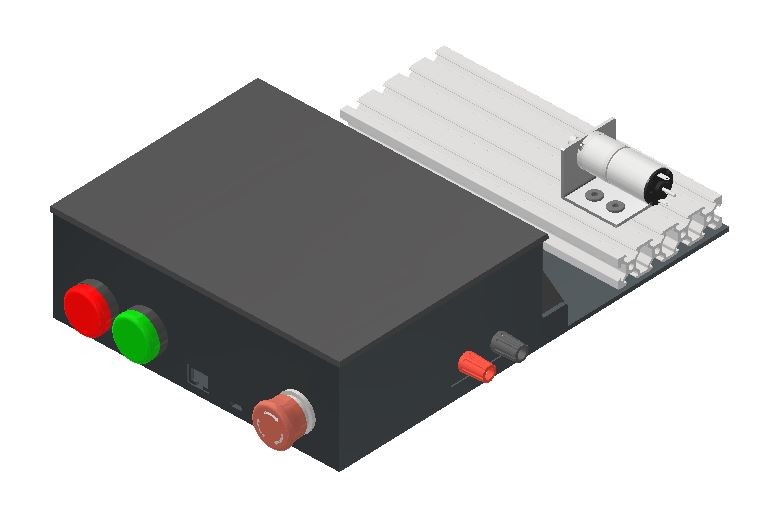
\includegraphics[width=0.92\linewidth]{CHPTRS/CH05_DIS_MECANICO/Fig/CAD1.JPG}
  \caption{Modelo CAD general del sistema mecánico del banco de pruebas.}
  \label{fig:cad_general_sistema}
\end{figure}

%============================================================
%============================================================
\section{Diseño de la carcasa y elementos de interfaz}
\label{sec:carcasa_elementos}

La carcasa del banco de pruebas se diseñó para proteger la electrónica, ordenar el cableado y centralizar los elementos de interacción del usuario durante la operación. En particular, se incorporaron alojamientos en el panel frontal para el montaje de los botones de encendido, apagado y parada de emergencia, cuyas dimensiones fueron medidas previamente en físico para asegurar un ajuste adecuado. Asimismo, se incluyeron conectores tipo banana para facilitar la conexión rápida de los terminales del motor bajo prueba y de la fuente externa de alimentación.

Estas consideraciones se ilustran en la Figura~\ref{fig:carcasa_interfaz_subfig}, donde se muestran (a) las perforaciones destinadas a los botones de control y (b) la disposición de los conectores tipo banana en el panel de conexiones.

\begin{figure}[H]
  \centering
  \begin{subfigure}[t]{0.48\textwidth}
    \centering
    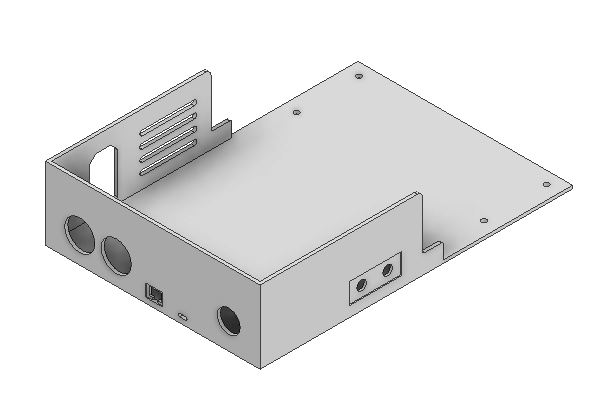
\includegraphics[width=\linewidth]{CHPTRS/CH05_DIS_MECANICO/Fig/carcasa.JPG}
    \caption{Perforaciones para botones de control y parada de emergencia.}
    \label{fig:carcasa_botones}
  \end{subfigure}
  \hfill
  \begin{subfigure}[t]{0.48\textwidth}
    \centering
    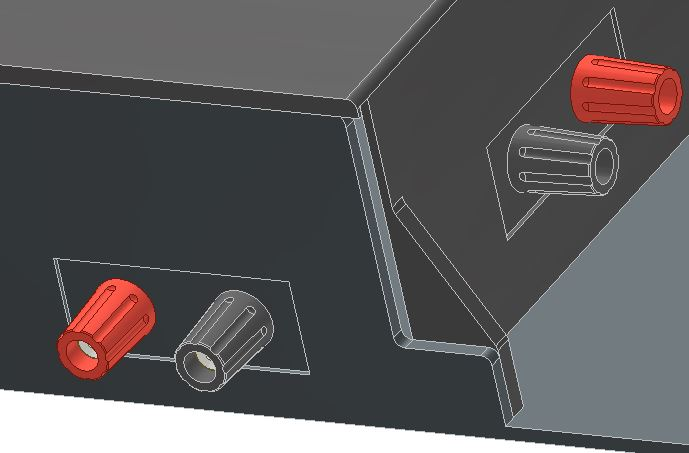
\includegraphics[width=\linewidth]{CHPTRS/CH05_DIS_MECANICO/Fig/CAD12.JPG}
    \caption{Conectores tipo banana para motor y alimentación externa.}
    \label{fig:carcasa_banana}
  \end{subfigure}
  \caption{Elementos principales de interfaz integrados en la carcasa.}
  \label{fig:carcasa_interfaz_subfig}
\end{figure}

Adicionalmente, la carcasa integra LEDs indicadores y puertos para carga de código y transferencia de datos, los cuales se presentan en la Figura~\ref{fig:carcasa_interfaz_usuario}. Estos elementos permiten supervisar el estado del sistema y habilitan la comunicación con la interfaz de usuario durante la toma de datos.

\begin{figure}[H]
  \centering
  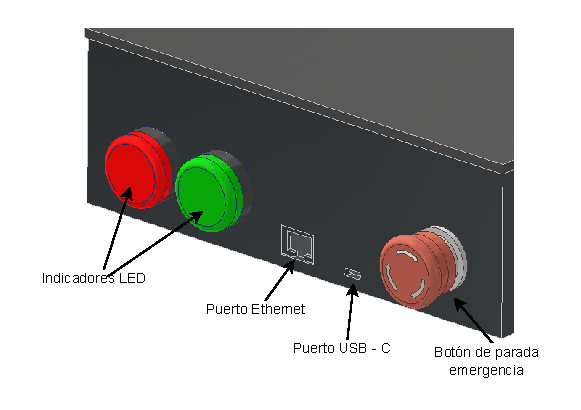
\includegraphics[width=0.85\linewidth]{CHPTRS/CH05_DIS_MECANICO/Fig/CAD10.pdf}
  \caption{Distribución de botones, LEDs indicadores y puertos de programación/datos en la carcasa.}
  \label{fig:carcasa_interfaz_usuario}
\end{figure}

Como medida adicional de protección, se incorpora un interruptor general de emergencia ubicado al inicio de la línea de alimentación del sistema. Este elemento permite el corte inmediato de energía y, además, integra un fusible para protección ante sobrecorriente, contribuyendo a resguardar el conjunto en caso de una falla eléctrica (p. ej., un cortocircuito). La disposición de este elemento se muestra en la Figura~\ref{fig:carcasa_switch_fusible}.

\begin{figure}[H]
  \centering
  % Reemplaza el nombre del archivo por el que usarás en tu tesis
  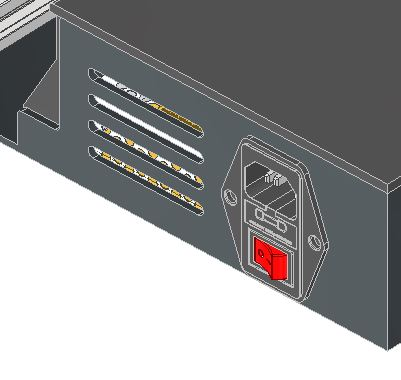
\includegraphics[width=0.55\linewidth]{CHPTRS/CH05_DIS_MECANICO/Fig/CAD11.JPG}
  \caption{Interruptor general con fusible integrado para corte y protección al inicio de la alimentación.}
  \label{fig:carcasa_switch_fusible}
\end{figure}
%============================================================


\subsection{Criterio simple de fijación carcasa--bancada}
\label{subsec:fijacion_carcasa_bancada}

La unión entre la carcasa (chapa metálica) y la bancada (perfil V-SLOT de aluminio) se realiza mediante cuatro apoyos, cada uno conformado por una unión atornillada con tuerca tipo martillo que genera presión sobre el perfil. La Figura~\ref{fig:fix_carcasa_vslot_detalle} muestra el detalle del ensamble empleado (tornillo, arandela, chapa y tuerca tipo martillo alojada en la ranura del perfil).

% ---------------------------------------------------------
% INSERTAR FIGURA: detalle de fijación carcasa--bancada
% ---------------------------------------------------------
\begin{figure}[H]
  \centering
  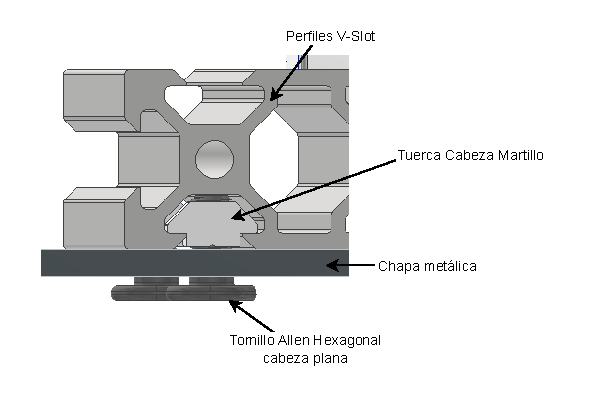
\includegraphics[width=0.6\linewidth]{CHPTRS/CH05_DIS_MECANICO/Fig/CAD8.drawio.pdf}
  \caption{Detalle de fijación carcasa--bancada mediante tornillo, arandela y tuerca tipo martillo sobre perfil V-SLOT.}
  \label{fig:fix_carcasa_vslot_detalle}
\end{figure}

Para estimar de forma preliminar la fuerza necesaria para que el conjunto deslice sobre el perfil (antes de reajustar la posición), se modela la resistencia al movimiento como fricción entre aluminio y acero (tuerca/tornillería). Para esta combinación, valores típicos reportados son \(\mu_s \approx 0.61\) (fricción estática) y \(\mu_k \approx 0.47\) (fricción cinética). \autocite{misumi_friction}

Si se considera que cada apoyo aporta una fuerza normal de apriete \(F_p\) (debida al ajuste del tornillo), la capacidad de fricción total puede aproximarse como:

\begin{align}
N_{\text{tot}} &\approx \sum_{i=1}^{4} F_{p,i} + W, \label{eq:ntot_fix}\\
F_{s,\max} &\approx \mu_s\,N_{\text{tot}}, \label{eq:fsmax_fix}\\
F_{k} &\approx \mu_k\,N_{\text{tot}}, \label{eq:fk_fix}
\end{align}

donde \(W\) es el peso total del subconjunto montado. En la práctica, cuando existe apriete, el término dominante suele ser \(\sum F_{p,i}\), por lo que \(W\) resulta secundario frente a la fuerza de sujeción.

\textit{Ejemplo numérico.} Suponiendo cuatro apoyos con un apriete moderado equivalente a \(F_{p,i}\approx 500~\mathrm{N}\) por apoyo, se obtiene \(N_{\text{tot}}\approx 2000~\mathrm{N}\) (despreciando \(W\) frente al apriete). Con ello:

\begin{align}
F_{s,\max} &\approx 0.61\,(2000)\approx 1220~\mathrm{N}, \label{eq:fsmax_num}\\
F_k &\approx 0.47\,(2000)\approx 940~\mathrm{N}. \label{eq:fk_num}
\end{align}

Este resultado respalda que, con cuatro puntos de fijación, el conjunto permanece estable ante esfuerzos de operación y vibración, y sólo deslizaría si se aplica una fuerza comparable a la indicada en la Ecuación~\eqref{eq:fsmax_num} o si se reduce el apriete. Cabe resaltar que \(\mu_s\) y \(\mu_k\) dependen del acabado superficial, limpieza y posible lubricación; por ello, estos valores se emplean como una referencia de diseño. \autocite{misumi_friction}



%============================================================
\section{Bancada de pruebas con perfiles V-SLOT}
\label{sec:bancada_vslot}

La bancada se implementa con perfiles de aluminio tipo V-SLOT de \(20\times 80~\mathrm{mm}\). Esta selección permite estandarizar los puntos de montaje mediante la ranura del perfil, facilitando el ajuste de posición de los soportes (brackets) y del conjunto del sensor. Adicionalmente, los perfiles presentan un acabado resistente y un ensamblaje práctico mediante tuercas cabeza de martillo y tornillos hexagonales de cabeza plana, lo que reduce el tiempo de reconfiguración durante pruebas con motores de geometrías distintas.

% ---------------------------------------------------------
% INSERTAR FIGURA: perfil V-SLOT 20x80 + detalle de ranura
% ---------------------------------------------------------
% \begin{figure}[H]
%   \centering
%   \includegraphics[width=0.85\linewidth]{CHPTRS/CH05_DIS_MECANICO/Fig/vslot_20x80.pdf}
%   \caption{Perfil V-SLOT de \(20\times 80~\mathrm{mm}\) empleado como bancada del banco de pruebas.}
%   \label{fig:vslot_20x80}
% \end{figure}

% ---------------------------------------------------------
% INSERTAR FIGURA: tuerca martillo + tornillo cabeza plana (detalle de sujeción)
% ---------------------------------------------------------
% \begin{figure}[H]
%   \centering
%   \includegraphics[width=0.85\linewidth]{CHPTRS/CH05_DIS_MECANICO/Fig/tnut_sujecion.pdf}
%   \caption{Sistema de fijación sobre perfil V-SLOT mediante tuerca tipo martillo y tornillería hexagonal.}
%   \label{fig:tnut_sujecion}
% \end{figure}

%============================================================
\section{Bracket de sujeción del motor y restricción de dimensiones}
\label{sec:bracket_motor}

Los brackets del motor se diseñan para sujetar el motor mediante los tornillos de su carcasa, manteniendo una fijación rígida y repetible variando unicamente los tornillos de fijación con la carcasa de los motores. Estos brackets se montan sobre la bancada V-SLOT utilizndo tuercas tipo martillo, lo que permite desplazar el motor a lo largo del perfil y ajustar su posición respecto al sensor.

Debido a la altura y geometría de la bancada (\(20\times 80~\mathrm{mm}\)), para motores de gran diámetro la sujeción puede requerir elevadores adicionales con el fin de alinear el eje del motor con el plano del sensor. En particular, conforme aumenta el diámetro del motor, aumenta la altura necesaria del bracket, reduciendo la rigidez del conjunto y aumentando la sensibilidad a vibración. Por este motivo, se establece una restricción práctica de dimensiones para los motores que se probarán, priorizando motores cuyos diámetros permitan el alineamiento sin incrementos excesivos de altura sobre la bancada.

% ---------------------------------------------------------
% INSERTAR FIGURA: bracket del motor montado sobre V-SLOT (vista CAD y/o foto)
% ---------------------------------------------------------
% \begin{figure}[H]
%   \centering
%   \includegraphics[width=0.85\linewidth]{CHPTRS/CH05_DIS_MECANICO/Fig/bracket_motor_vslot.pdf}
%   \caption{Bracket de sujeción del motor fijado sobre la bancada V-SLOT.}
%   \label{fig:bracket_motor_vslot}
% \end{figure}

%============================================================
\section{Mecanismo de transmisión y acople solidario al eje}
\label{sec:mecanismo_transmision}

Para transmitir el giro del eje hacia el conjunto de sensado se emplea un acople de geometría simple inspirado en bujes comerciales, diseñado para montarse solidario al eje y asegurar la repetibilidad del montaje. Esta solución permite escalar la geometría del acople a distintos diámetros de eje, manteniendo el mismo principio de fijación mediante tornillo prisionero.

En este trabajo se consideran ejes de \(4~\mathrm{mm}\) y \(6~\mathrm{mm}\), por lo que se diseñan variantes del acople con el diámetro interno correspondiente. Con el fin de estandarizar la tornillería del conjunto, el acople y el soporte del imán se preparan para roscas M3, empleando un macho para generar la rosca durante el prototipado. Además, dado que la estimación de parámetros requiere considerar la inercia total acoplada al eje, se priorizan geometrías compactas que minimicen masa adicional.

\begin{figure}[H]
    \centering
    \begin{tabularx}{\linewidth}{>{\centering\arraybackslash}X}
        \begin{subfigure}[t]{0.55\linewidth}
            \centering
            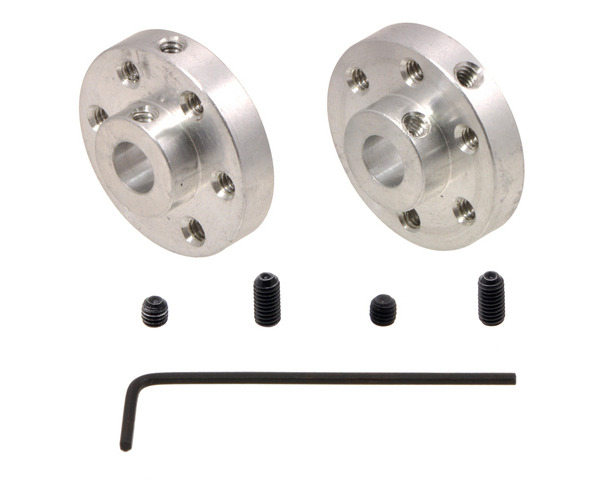
\includegraphics[width=\linewidth]{CHPTRS/CH03_DICON/Fig/CH03_FIG03_SolucionOptima/04a_SO_MotorPololu1.jpg}
        \end{subfigure}
    \end{tabularx}
    \caption{Bujes de fijación referenciales (inspiración para el acople del eje).}
    \label{fig:bujes_referenciales}
\end{figure}

% ---------------------------------------------------------
% INSERTAR FIGURA: acople para eje 4 mm y 6 mm (dos vistas)
% ---------------------------------------------------------
\begin{figure}[H]
  \centering
  \begin{subfigure}[t]{0.48\textwidth}
    \centering
    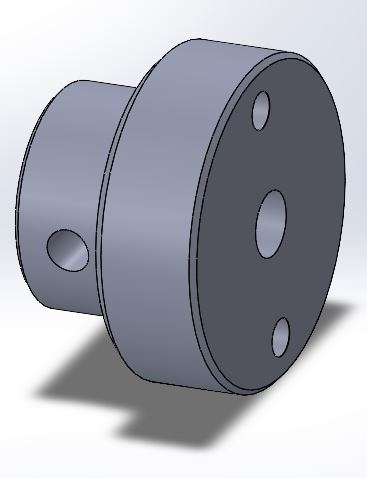
\includegraphics[width=0.65\linewidth]{CHPTRS/CH05_DIS_MECANICO/Fig/01a_AcopleIman.JPG}
    \caption{Acople para eje de 4 mm.}
    \label{fig:acople_4mm}
  \end{subfigure}
  \hfill
  \begin{subfigure}[t]{0.48\textwidth}
    \centering
    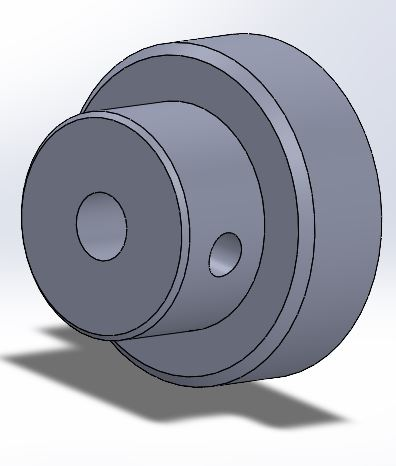
\includegraphics[width=0.65\linewidth]{CHPTRS/CH05_DIS_MECANICO/Fig/01b_AcopleIman.JPG}
    \caption{Acople para eje de 6 mm.}
    \label{fig:acople_6mm}
  \end{subfigure}
  \caption{Variantes del acople para distintos diámetros de eje.}
  \label{fig:acoples_eje}
\end{figure}

El acople incluye puntos de fijación para un soporte destinado a posicionar el imán de neodimio de forma concéntrica con el eje. 
% La Figura~\ref{fig:soporte_iman_acople} muestra la pieza diseñada para fijarse al acople y alojar el imán, manteniéndolo expuesto y próximo al sensor.

% \begin{figure}[H]
%   \centering
%   \begin{tabularx}{\linewidth}{>{\centering\arraybackslash}X}
%     \begin{subfigure}[t]{0.60\linewidth}
%       \centering
%       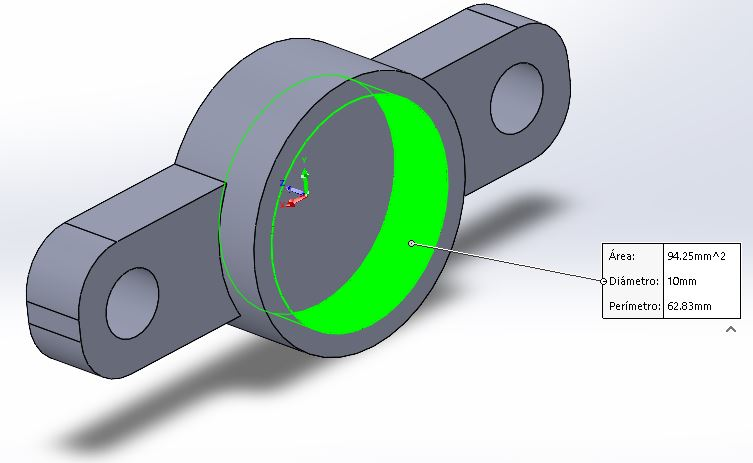
\includegraphics[width=\linewidth]{CHPTRS/CH05_DIS_MECANICO/Fig/02_SoporteIman.JPG}
%     \end{subfigure}
%   \end{tabularx}
%   \caption{Soporte de imán diseñado para fijarse al acople solidario al eje.}
%   \label{fig:soporte_iman_acople}
% \end{figure}

\begin{figure}[H]
  \centering
  \begin{tabularx}{\linewidth}{>{\centering\arraybackslash}X}
    \begin{subfigure}[t]{0.55\linewidth}
      \centering
      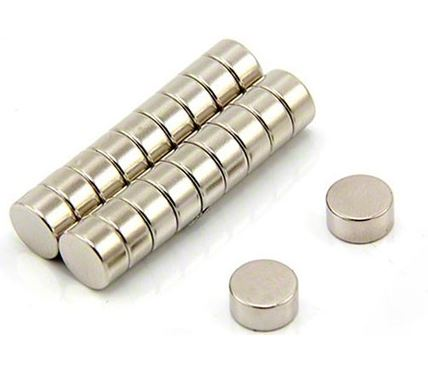
\includegraphics[width=\linewidth]{CHPTRS/CH05_DIS_MECANICO/Fig/CAD9.JPG}
    \end{subfigure}
  \end{tabularx}
  \caption{Imán de neodimio seleccionado para las pruebas (diámetro nominal \(5~\mathrm{mm}\)).}
  \label{fig:iman_neodimio}
\end{figure}

Para la etapa de prototipado y validación, estas piezas se fabrican mediante impresión 3D y se evalúan en el Capítulo~\ref{ch:CH07}. Para la solución final, se considera emplear un material no magnético, como por ejemplo, aluminio, con el fin de no alterar el campo del imán durante el sensado.

%============================================================
\section{Estructura de fijación del sensor de efecto \textit{hall}}
\label{sec:estructura_sensor_hall}

El sensado de posición angular y velocidad angular se realiza mediante el integrado TMAG5170. Para garantizar mediciones consistentes, la \ac{PCB} del sensor debe fijarse sobre una estructura rígida que permita ubicar el sednsor TMAG5170 de manera coaxial con el eje del motor. Adicionalmente, se busca que el conjunto sea simétrico respecto a la bancada, de modo que el eje del motor pueda posicionarse centrado y el sensado se realice en condiciones geométricas repetibles.

\subsection{Principio de funcionamiento y criterio de alineamiento}
\label{subsec:funcionamiento_tmag}

El TMAG5170 estima el ángulo a partir de la variación del campo magnético en el plano \(XY\). Por ello, se emplea un imán de neodimio polarizado montado solidario al eje del motor, de modo que la orientación magnética varíe con el giro. En la Figura~\ref{fig:tmag_magnet_setup} se presenta un esquema de referencia para el montaje del imán y, adicionalmente, la ubicación de la zona activa del sensor dentro del integrado, la cual se utiliza como referencia para el alineamiento.

\begin{figure}[H]
\centering
\begin{subfigure}[t]{0.48\textwidth}
    \centering
    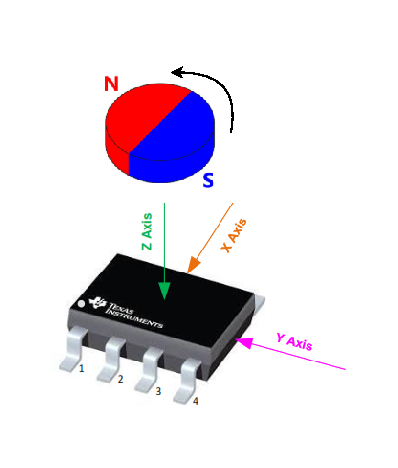
\includegraphics[width=\linewidth]{CHPTRS/CH05_DIS_MECANICO/Fig/CAD6.pdf}
    \caption{Esquema de referencia para el montaje del imán respecto al sensor.}
    \label{fig:tmag_magnet_scheme}
\end{subfigure}
\hfill
\begin{subfigure}[t]{0.48\textwidth}
    \centering
    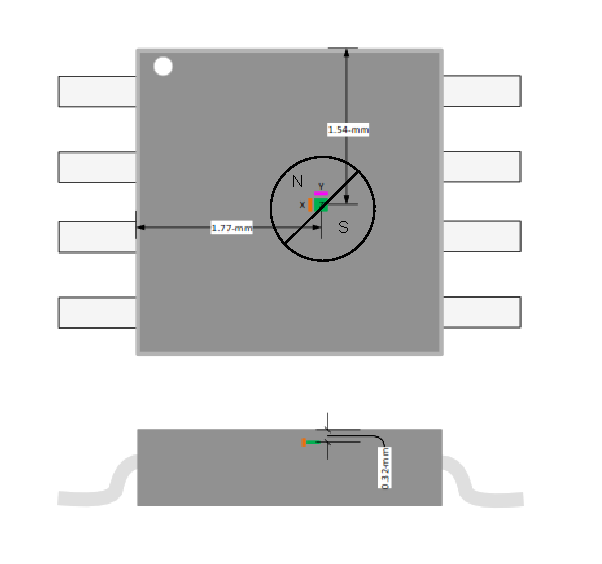
\includegraphics[width=\linewidth]{CHPTRS/CH05_DIS_MECANICO/Fig/CAD7.pdf}
    \caption{Ubicación aproximada de la zona activa del sensor de efecto \textit{hall} en el integrado.}
    \label{fig:tmag_hall_location}
\end{subfigure}
\caption{Referencia de montaje del imán y ubicación del sensor en el TMAG5170.}
\label{fig:tmag_magnet_setup}
\end{figure}

\subsection{Selección del imán}
\label{subsec:seleccion_iman_mec}

Con base en las pruebas documentadas en el Capítulo~\ref{ch:CH07}, se evaluaron imanes de distintos tamaños para mejorar la estabilidad del sensado. Considerando que el TMAG5170 tiene dimensiones reducidas (del orden de \(3~\mathrm{mm}\times 3~\mathrm{mm}\)), se observó que imanes muy grandes incrementan la sensibilidad a desalineamientos y pueden degradar la coherencia de la medición. En contraste, el imán de \(5~\mathrm{mm}\) de diámetro presentó un desempeño más estable, al facilitar el alineamiento del conjunto imán--sensor y mejorar la repetibilidad de la estimación de ángulo.

% ---------------------------------------------------------
% INSERTAR FIGURA: soporte completo PCB sensor + ajuste de distancia al imán (vista CAD)
% ---------------------------------------------------------
% \begin{figure}[H]
%   \centering
%   \includegraphics[width=0.85\linewidth]{CHPTRS/CH05_DIS_MECANICO/Fig/soporte_pcb_sensor.pdf}
%   \caption{Estructura de fijación de la \ac{PCB} del TMAG5170 y referencia de su alineamiento coaxial con el eje del motor.}
%   \label{fig:soporte_pcb_sensor}
% \end{figure}

%============================================================
% Nota para ti (no es parte del texto final si no quieres):
% Figuras sugeridas por sección (para que las consigas):
% - Carcasa: CAD del panel frontal, detalle LEDs/puertos, conectores banana, distribución interna.
% - Bancada V-SLOT: perfil 20x80, tuerca martillo + tornillo, vista de montaje sobre bancada.
% - Brackets: bracket montado, ejemplo motor pequeño vs motor grande (comparativa de altura).
% - Transmisión: acoples 4 mm y 6 mm, soporte del imán, imán real.
% - Sensor hall: soporte de PCB, esquema de coaxialidad, referencia de distancia imán--sensor.
%============================================================
         \cleardoublepage
\chapter{Diseño del \ac{SW} del sistema}
\ihead[]{Capítulo 6: Diseño \ac{SW} del sistema}
\label{ch:CH06_Diseno-software}
%%%%%%%%%%%%%%%%%%%%%%%%%%%%%%%%%%%%%%%%%%

\section{Diseño de la interfaz}
\section{Inicialización del sistema y funcionamiento de envió de parámetros}
\section{Protocolo de comunicación con el HW}
\section{Desarrollo del algoritmo de mínimos cuadrados para la estimación}
\section{Diagrmas de flujo de la lógica e control del sistema}                \cleardoublepage
\chapter{Implementación y pruebas del prototipo}
\ihead[]{Capítulo 7: Implementación del prototipo}
\label{ch:CH07}
%%%%%%%%%%%%%%%%%%%%%%%%%%%%%%%%%%%%%%%%%%

\noindent
En este capítulo se recopilan las pruebas realizadas con un prototipo, con el objetivo de validar el funcionamiento del diseño electrónico y mecánico, así como del \ac{SW}, para lograr una implementación correcta de la solución general planteada en los Capítulos~\ref{ch:CH04}, \ref{ch:CH05} y \ref{ch:CH06}. En primer lugar, se presentan las pruebas y configuraciones de los componentes que conforman el \ac{HW}, empleando elementos de prototipado rápido, como piezas fabricadas mediante impresión 3D y placas perforadas para el montaje electrónico. En cuanto al \ac{SW} de la solución, se muestran fragmentos representativos del código, con énfasis en la lógica de recepción y envío de datos.
\section{Desarrollo de la tarjeta}

\noindent
Con el objetivo de acelerar la validación experimental del sistema, en esta etapa se emplea una placa de pruebas en lugar de la \ac{PCB} diseñada en el Capítulo~\ref{ch:CH04}. Esta decisión permite prototipar e iterar rápidamente sobre los valores de los componentes dimensionados en dicho capítulo, facilitando ajustes durante las primeras pruebas de funcionamiento. Aun cuando la implementación física se realiza sobre una placa de pruebas, se mantienen los mismos pines y conexiones definidos en el Capítulo~\ref{ch:CH04}, de modo que la migración posterior a la \ac{PCB} no implique cambios en la asignación de señales.

\noindent
Asimismo, esta configuración permite validar la comunicación del microcontrolador con la interfaz de operación del sistema, así como verificar el desempeño de los bloques principales de sensado y actuación. En particular, tal como se observa en la Figura~\ref{fig:pcb_pruebas_prototipo}, se implementan los componentes más relevantes para la etapa de pruebas: el sensor de efecto Hall y el \textit{driver} para el control de los motores que serán sensados. En las siguientes secciones se detalla el funcionamiento de la placa de pruebas diseñada para la implementación del prototipo.

% ---------------------------------------------------------
% INSERTAR FIGURA: placa de pruebas del prototipo
% ---------------------------------------------------------
\begin{figure}[H]
  \centering
  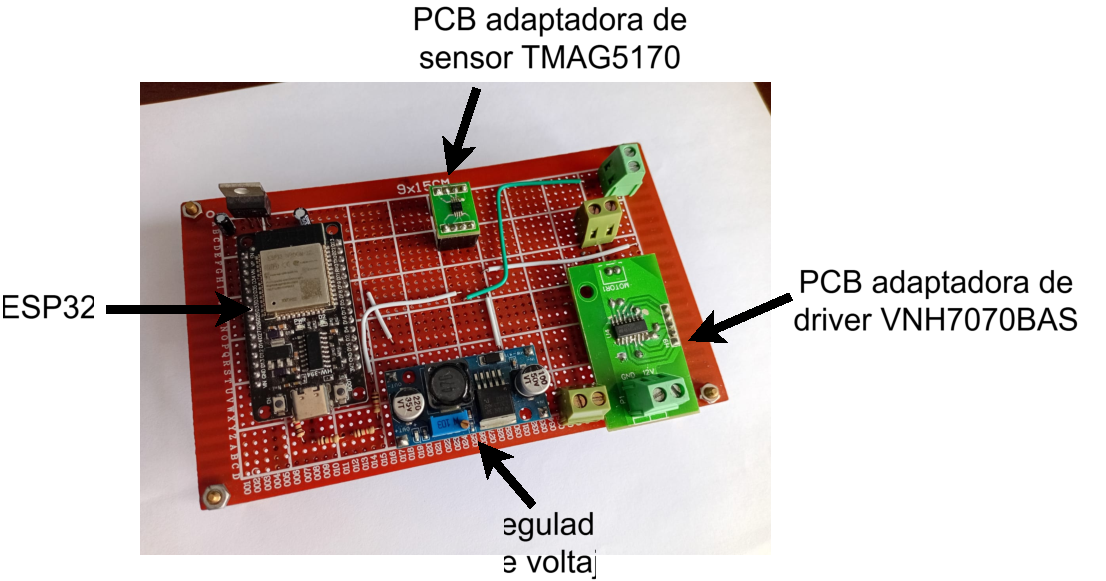
\includegraphics[width=0.90\linewidth]{CHPTRS/CH07_IMPLEMENTACION/Fig/hw_total_partes.pdf}
  \caption{Placa de pruebas diseñada para la implementación del prototipo.}
  \label{fig:pcb_pruebas_prototipo}
\end{figure}


\section{Prueba del sensor Hall}
\label{sec:prueba_sensor_hall}

\noindent
En esta sección se presentan las pruebas realizadas para la configuración del sensor de efecto Hall TMAG5170A1. Se muestran los componentes utilizados durante el montaje de prueba, los registros que deben editarse para su configuración y, finalmente, los resultados obtenidos en las pruebas realizadas con este sensor.

\subsection{Configuración mínima del TMAG5170A1 para detección de giro en el plano \(XY\)}

\noindent
Para las pruebas del sensor se empleó una \ac{PCB} de pruebas, mostrada en la Figura~\ref{fig:tmag_pcb_poc}, cuya finalidad es facilitar la integración del integrado en una placa de pruebas y permitir su conexión adecuada al microcontrolador. La implementación del montaje se muestra en la Figura~\ref{fig:tmag_pcb_poc}. Asimismo, se procuró validar cada componente y su circuito asociado de manera incremental, siguiendo los diseños presentados previamente en el Capítulo~\ref{ch:CH04}. La implementación del montaje se muestra en la Figura~\ref{fig:tmag_pcb_poc}. Para estas pruebas se procuró validar cada componente junto con su circuito asociado, previamente diseñado en el Capítulo~\ref{ch:CH04}.
 % ---- Figura: izquierda EasyEDA / derecha implementación ----
    % Requiere: \usepackage{subcaption}

\begin{figure}[H]
  \centering

  \begin{subfigure}[t]{0.48\textwidth}
    \centering
    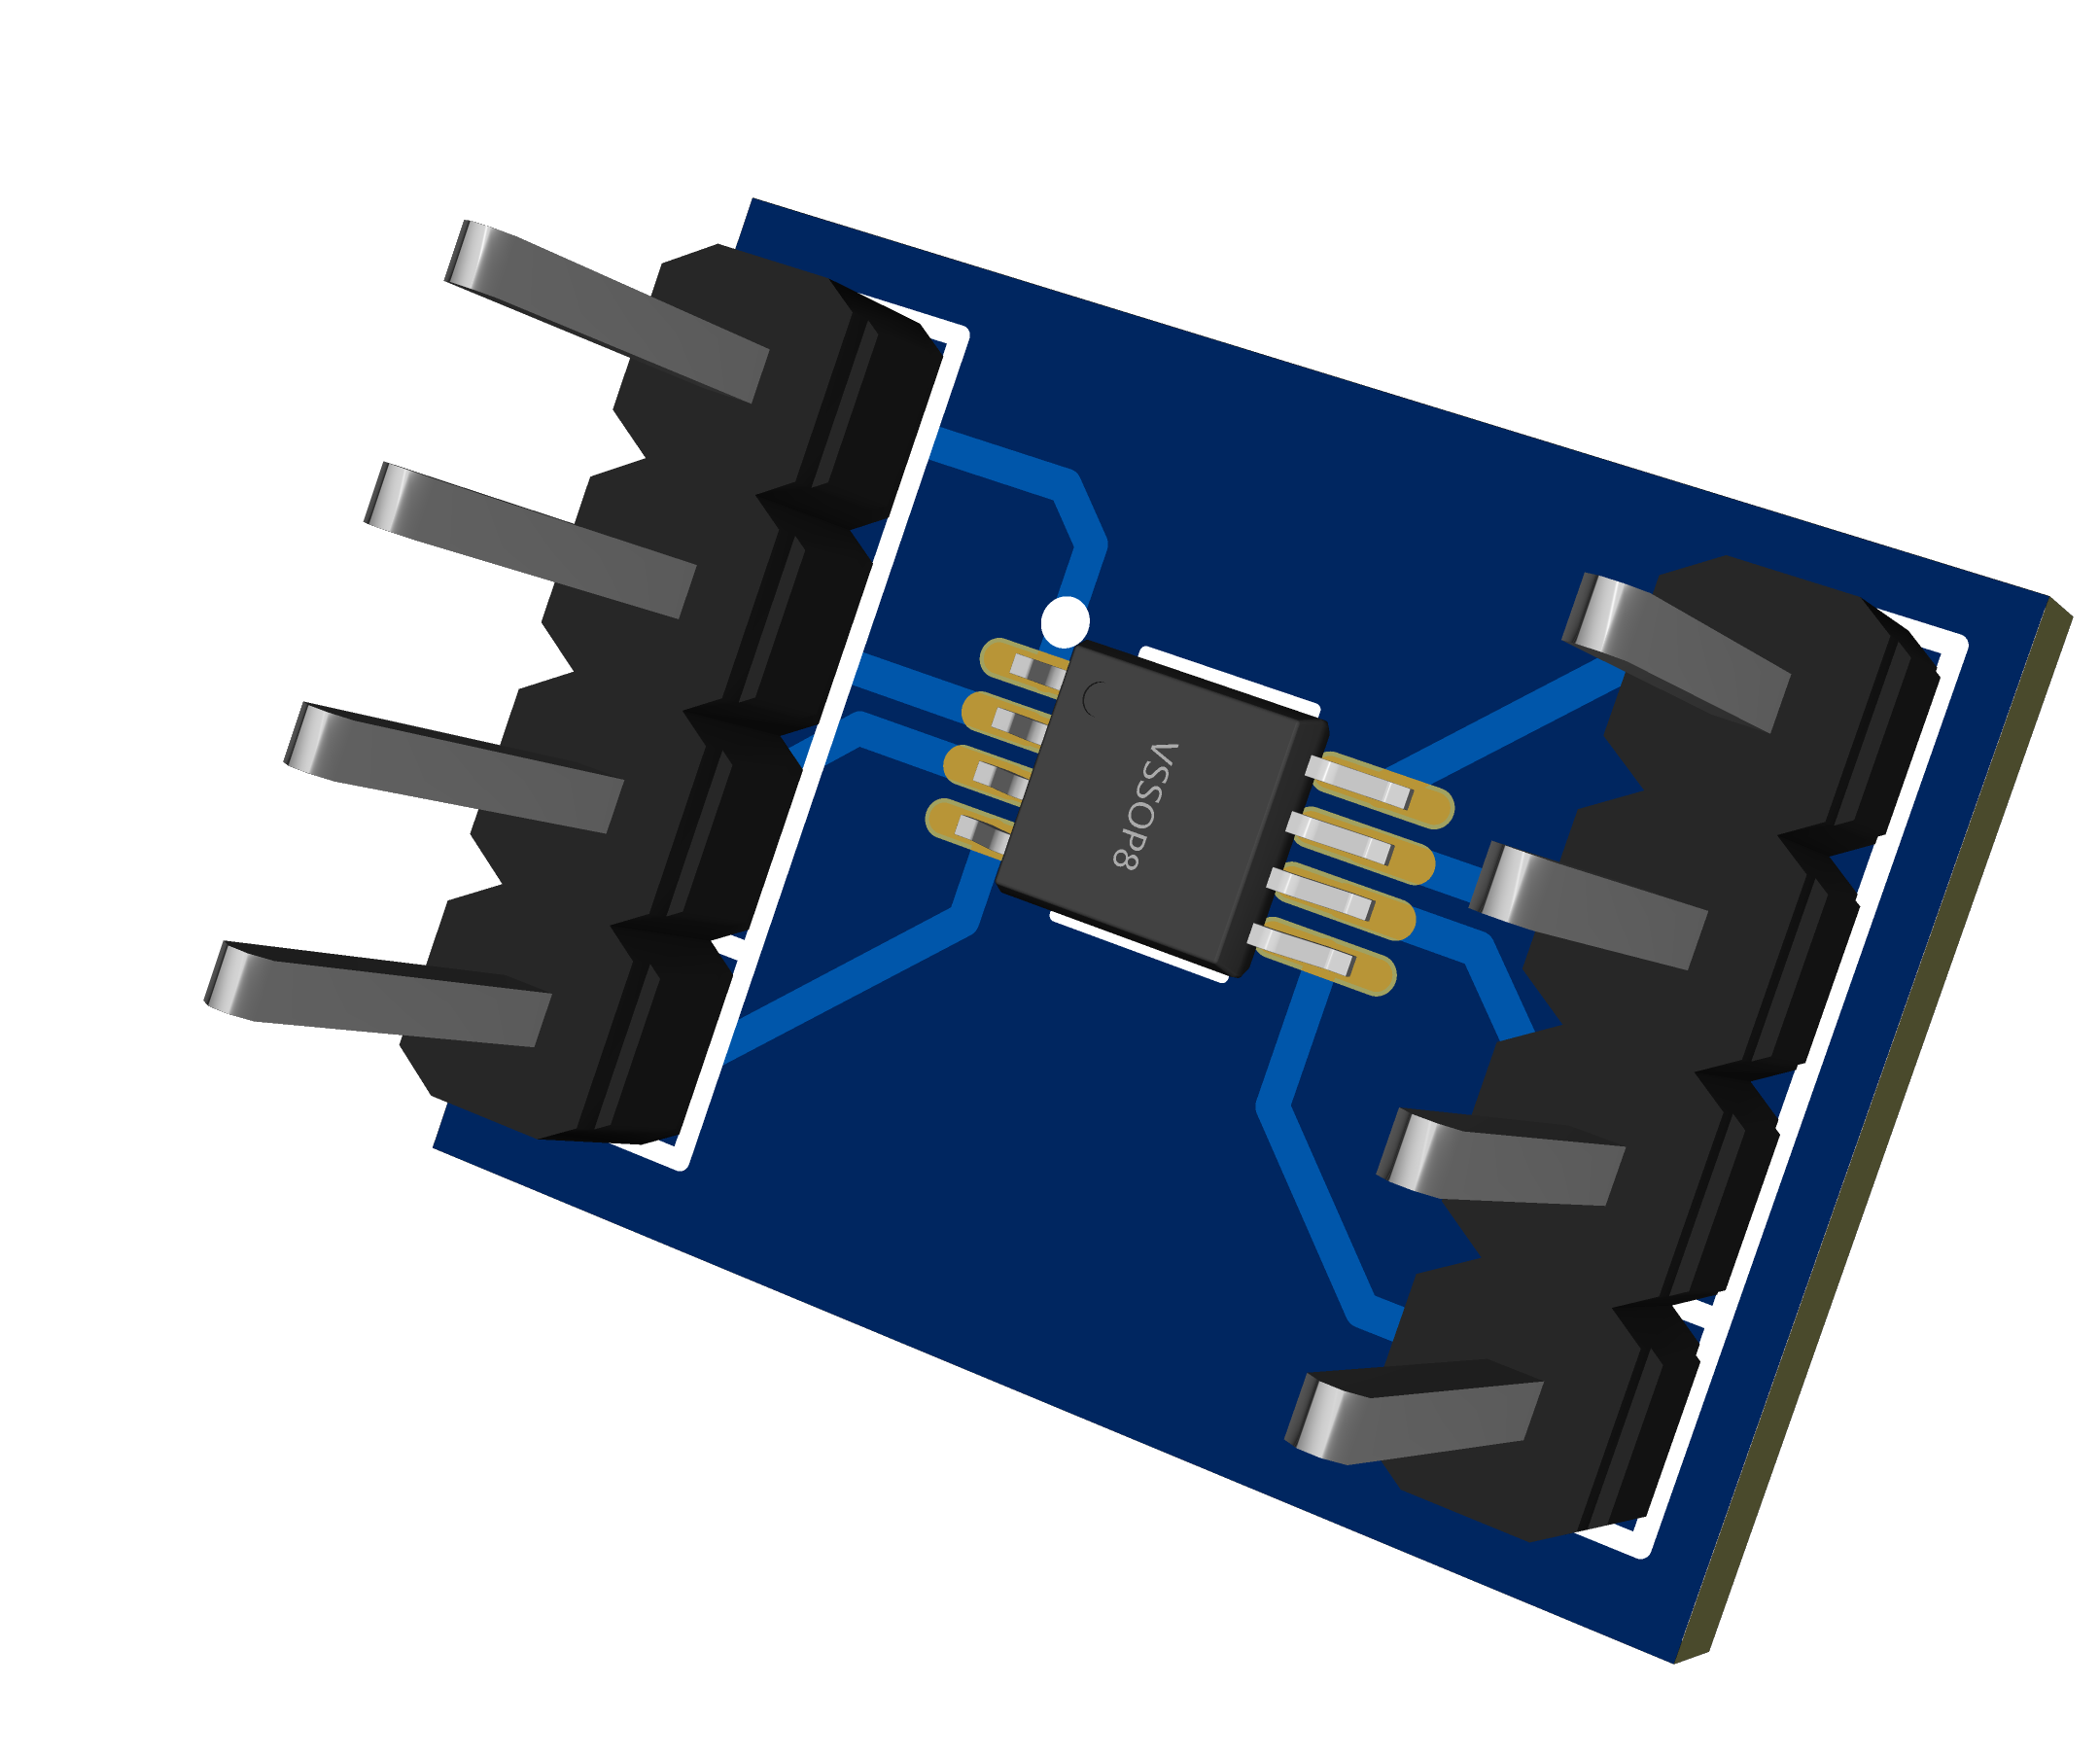
\includegraphics[width=\linewidth]{CHPTRS/CH07_IMPLEMENTACION/Fig/3D_PCB_TMAG.png}
    \caption{Diseño de la \ac{PCB} en EasyEDA.}
    \label{fig:diseñoPCBadapctacion}
  \end{subfigure}
  \hfill
  \begin{subfigure}[t]{0.48\textwidth}
    \centering
    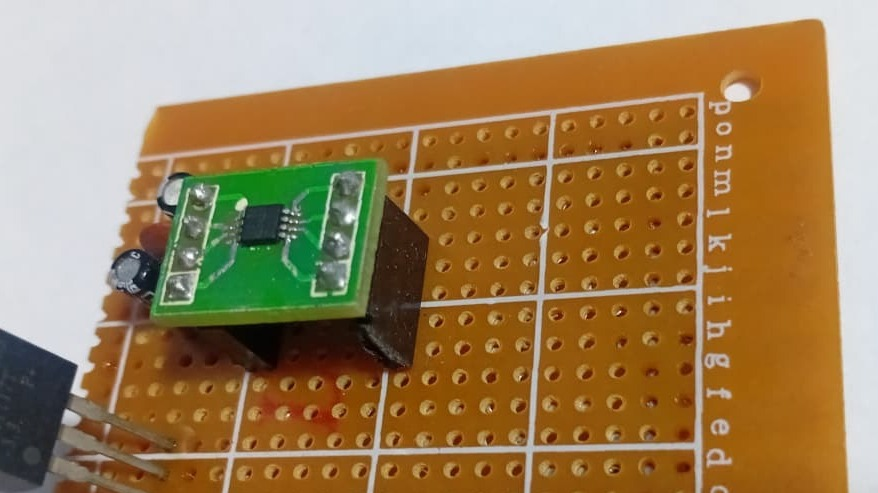
\includegraphics[width=\linewidth]{CHPTRS/CH07_IMPLEMENTACION/Fig/TMAG5170.jpeg}
    \caption{Implementación de la \ac{PCB} para pruebas.}
    \label{fig:implementacionsensor}
  \end{subfigure}

  \caption{\ac{PCB} para pruebas y configuración del sensor TMAG5170.}
  \label{fig:tmag_pcb_poc}
  \caption*{\footnotesize\textit{Nota: Componentes cortesía del profesor Enrique Vidal.}}
\end{figure}

\noindent
En este montaje se utiliza un regulador de \(3.3\,\text{V}\), el cual alimenta al sensor con el mismo nivel de tensión lógica que el microcontrolador ESP32. Para las pruebas se utilizó un módulo de desarrollo de este microcontrolador, el cual también será empleado  en la solución final.


\noindent
Según lo presentado en la Tabla~\ref{tab:pines_pcb}, se seleccionaron los pines 18, 19, 23 y 22 para la comunicación \ac{SPI} con el sensor (SCK, MISO, MOSI y CS, respectivamente). La configuración mínima del TMAG5170A1 se realizó mediante la escritura de registros internos. En particular, se deshabilitó el cálculo de CRC a través del registro de prueba y se habilitaron los canales \(X\), \(Y\) y \(Z\) con un rango de medición de \(\pm 100\,\text{mT}\), manteniendo el sistema en una configuración base para el sensado.

\noindent
En la Tabla~\ref{tabla_registros_tmag} se resumen los registros editados y los valores asignados en hexadecimal.

% ---------------------------------------------------------
% Tabla de registros configurados
% ---------------------------------------------------------
\begin{longtblr}[
  theme=pucp,
  label   = {tabla_registros_tmag},
  caption = {Registros configurados del TMAG5170A1 para sensado y estimación de ángulo en \(XY\).},
]{
  width=\linewidth,
  colspec = {Q[l,m,wd=0.30\linewidth] X[l,m] Q[c,m,wd=0.18\linewidth]},
  colsep=2pt,
  rowsep=1pt,
  rows={font=\footnotesize},
  row{1}={font=\footnotesize\bfseries,halign=c},
  rowhead=1, rowfoot=0,
  hlines, vlines,
}
Registro &
Descripción &
Valor escrito (hex) \\

\texttt{REG\_TEST\_CONFIG} \texttt{(0x0F)} &
Registro de prueba; se deshabilita CRC en la comunicación \ac{SPI} durante la etapa de pruebas. &
\texttt{0x000407} \\

\texttt{REG\_DEVICE\_CONFIG} \texttt{(0x00)} &
Configuración general del dispositivo; en esta prueba se habilita el modo de medición activo. &
\texttt{0x0020} \\

\texttt{REG\_SENSOR\_CONFIG} \texttt{(0x01)} &
Configuración del sensor; habilita los ejes \(X\), \(Y\) y \(Z\) y define el rango de medición del campo magnético. &
\texttt{0x41EA} \\

\texttt{REG\_SYSTEM\_CONFIG} \texttt{(0x02)} &
Configuración del sistema; para esta prueba mínima se mantiene el valor base. &
\texttt{0x0000} \\

\end{longtblr}

\noindent
Una vez aplicada la configuración, se realizó la lectura de los registros de resultado de \(X\), \(Y\) y \(Z\). Con estas mediciones se calculó el ángulo en el plano \(XY\) mediante \(\theta=\mathrm{atan2}(Y,X)\) y se ajustó su rango a \([0, 360]\,\text{grados}\). Para evitar discontinuidades al cruzar \(0/360^\circ\), se aplicó un ajuste de la variación angular para mantener la diferencia entre muestras dentro de \([-180,180]\) grados. Finalmente, la velocidad angular se obtiene como \(\omega=\Delta\theta/\Delta t\) y se convirtió a \(\text{rad}/\text{s}\).

\noindent
El sensor traduce la variación del campo magnético en una estimación de la posición angular en el eje solidario del motor. A partir de esta señal, se calcula la velocidad angular mediante la derivada temporal de la posición angular, como se muestra en la Figura~\ref{fig:graph_ang}.

% INSERTAR FIGURA: gráfica de ángulo y velocidad angular
\begin{figure}[ht!]
  \centering
  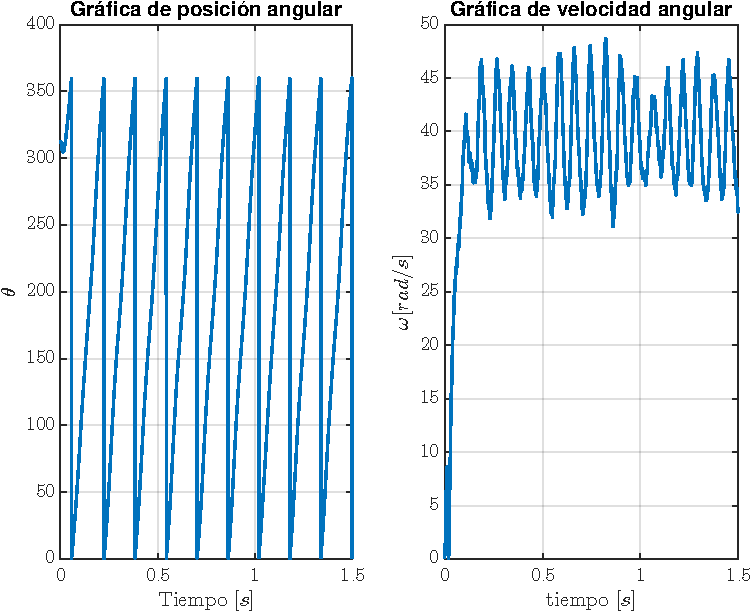
\includegraphics[width=0.95\linewidth]{CHPTRS/CH07_IMPLEMENTACION/Fig/ang_graph.pdf}
  \caption{Señales de posición angular y velocidad angular obtenidas a partir del TMAG5170A1.}
  \label{fig:graph_ang}
\end{figure}

\noindent
Para esta toma de datos no se utilizó ningún soporte mecánico, por lo que la señal de velocidad presenta ruido y no converge a un valor específico. Este comportamiento puede deberse a las vibraciones generadas durante la medición, principalmente por el movimiento de la mano al acercar el eje del motor con el imán hacia el sensor.
 
\section{Pruebas con el driver de motor}
\label{sec:pruebas_driver}

\noindent
Para las pruebas con el driver VNH7070BAS se empleó una etapa de potencia basada en el puente H seleccionado en el Capítulo~\ref{ch:CH04}, con el objetivo de validar su funcionamiento antes de integrarlo al prototipo final. En esta etapa se verificó la correcta excitación del motor \ac{DC} mediante señales de control provenientes de la ESP32 (habilitación, sentido de giro y \ac{PWM}), así como la lectura de la salida de sensado CS para su posterior adquisición por el ADC. Las pruebas se realizaron en un entorno de prototipado rápido, utilizando conexiones accesibles y puntos de medición que permiten observar las señales principales del driver y confirmar su compatibilidad con la lógica a \SI{3.3}{\volt} del microcontrolador.

% Requiere: \usepackage{subcaption}

\begin{figure}[H]
  \centering

  \begin{subfigure}[t]{0.48\textwidth}
    \centering
    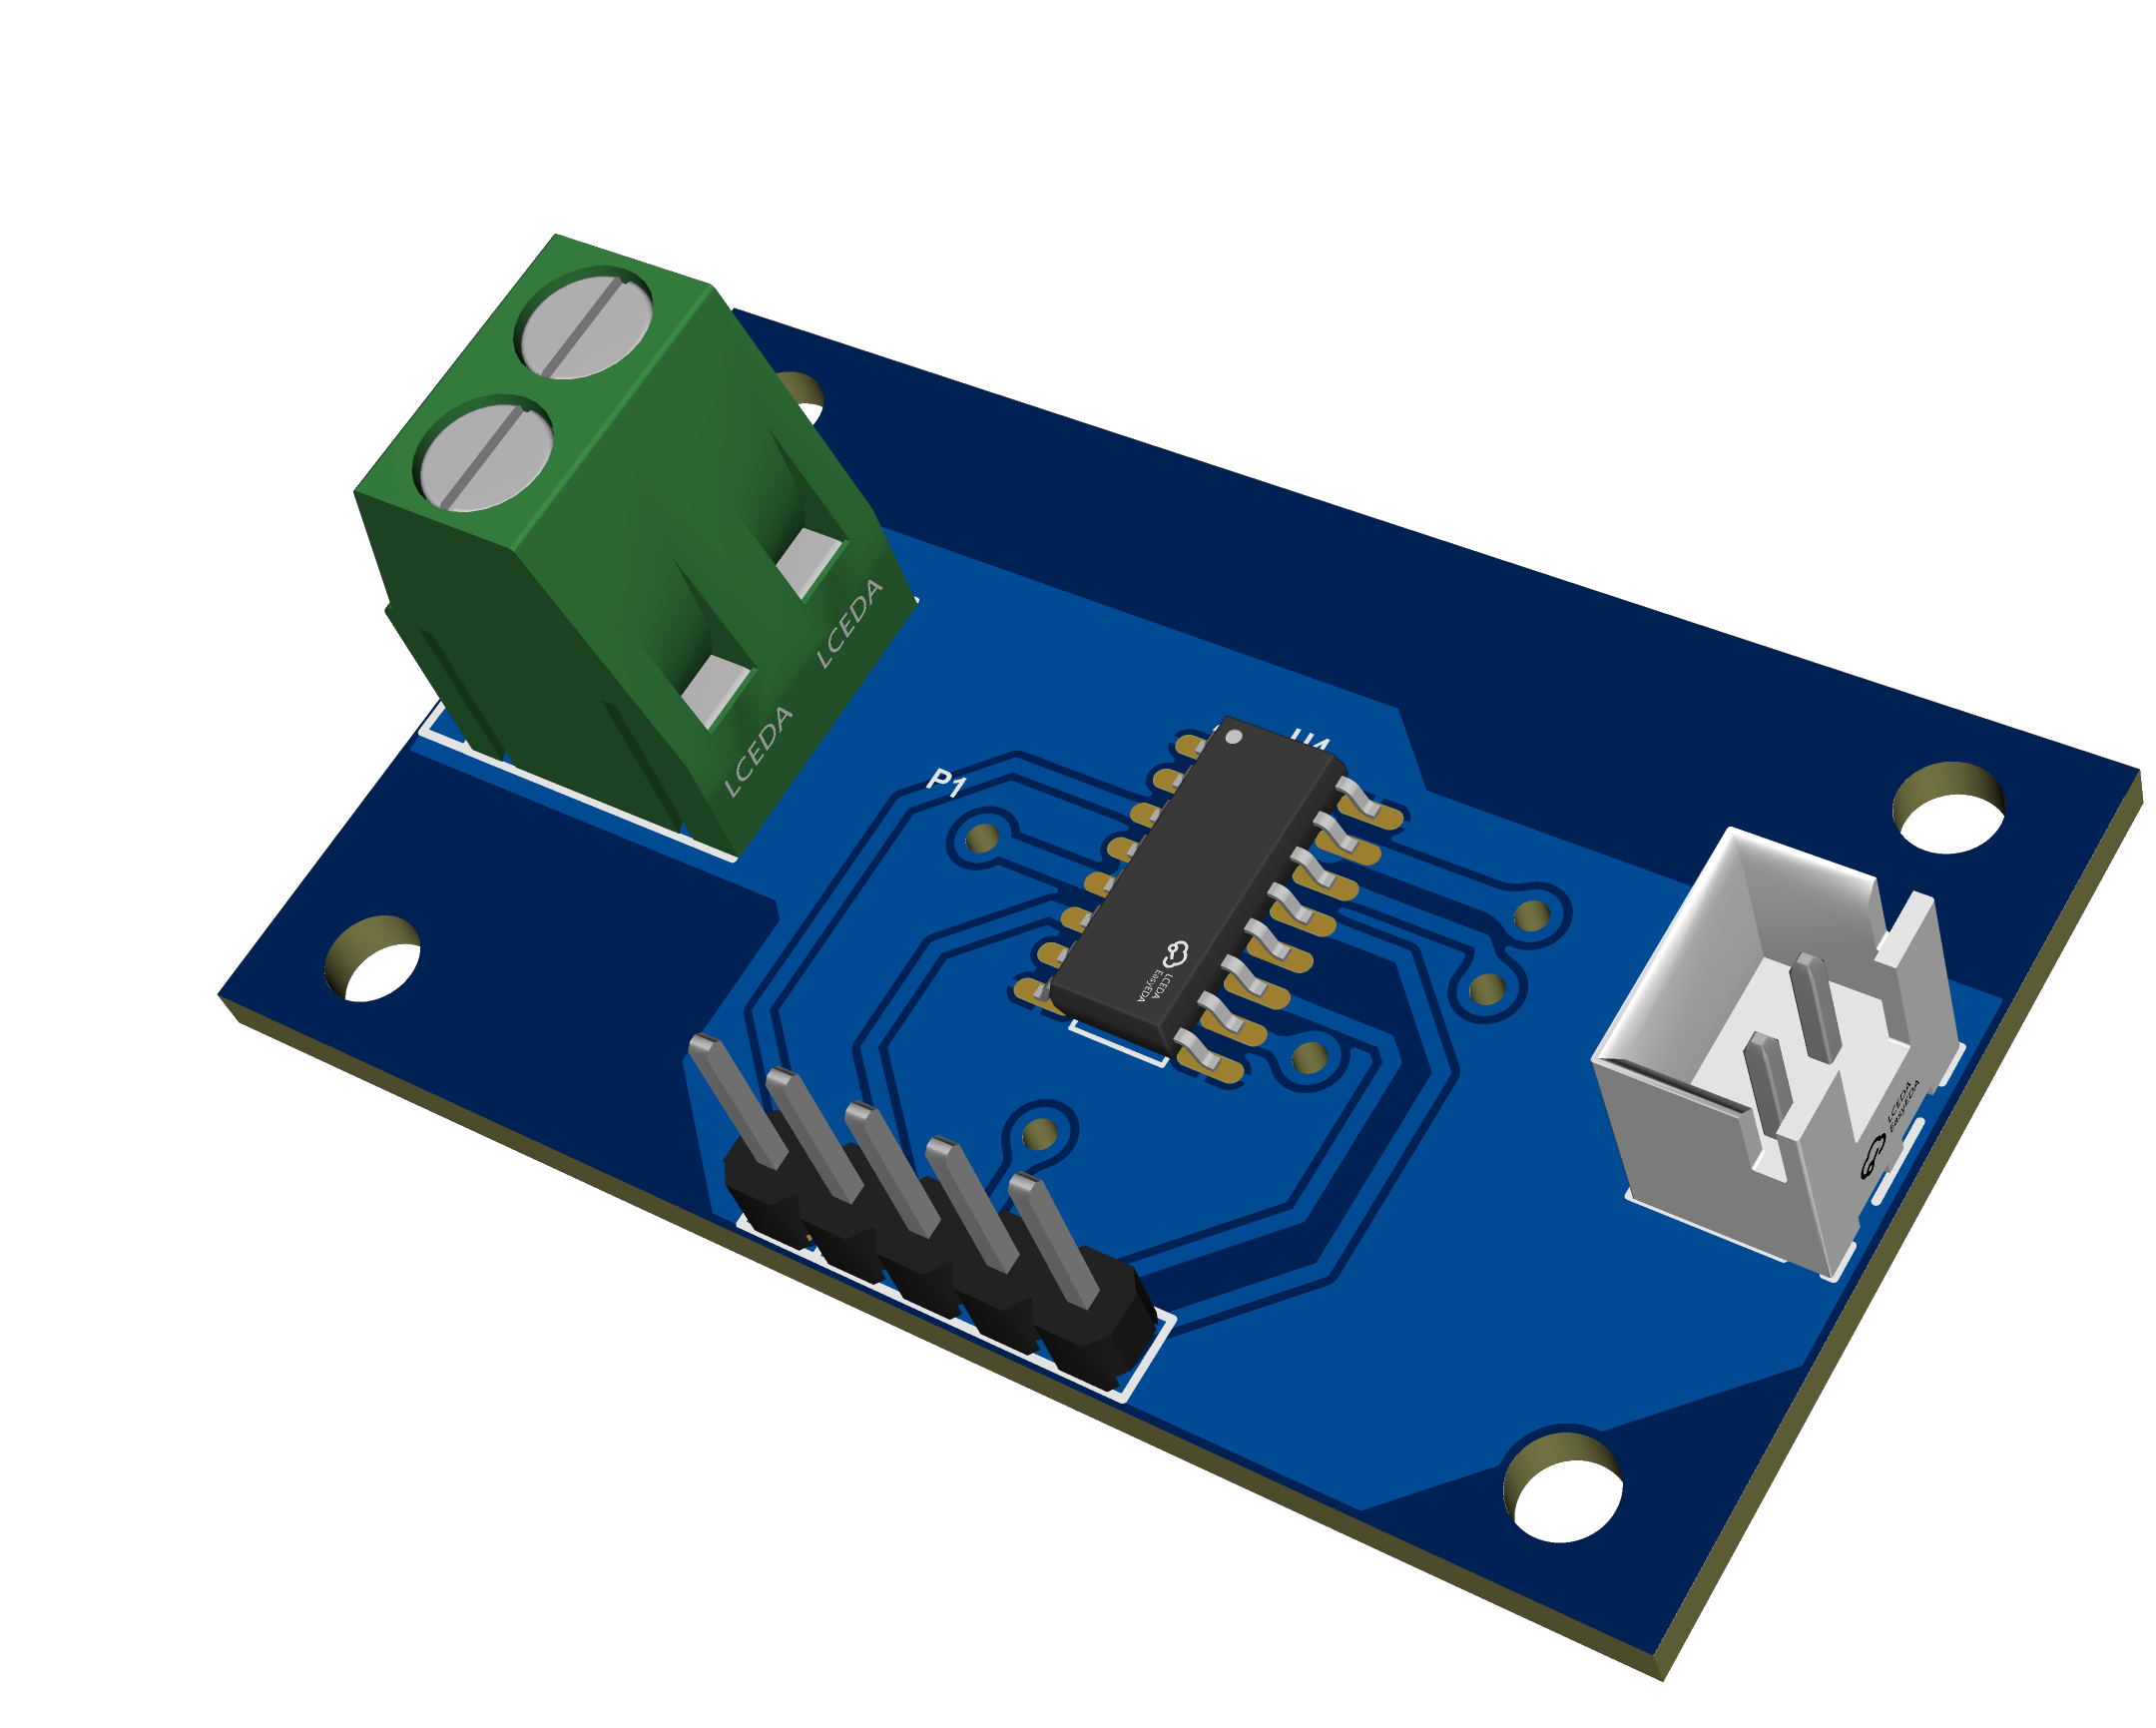
\includegraphics[width=\linewidth]{CHPTRS/CH07_IMPLEMENTACION/Fig/3D_PCB5_VNH.png}
    \caption{Diseño de la \ac{PCB} del driver VNH7070BAS en EasyEDA.}
    \label{fig:vnh_pcb_diseno}
  \end{subfigure}
  \hfill
  \begin{subfigure}[t]{0.48\textwidth}
    \centering
    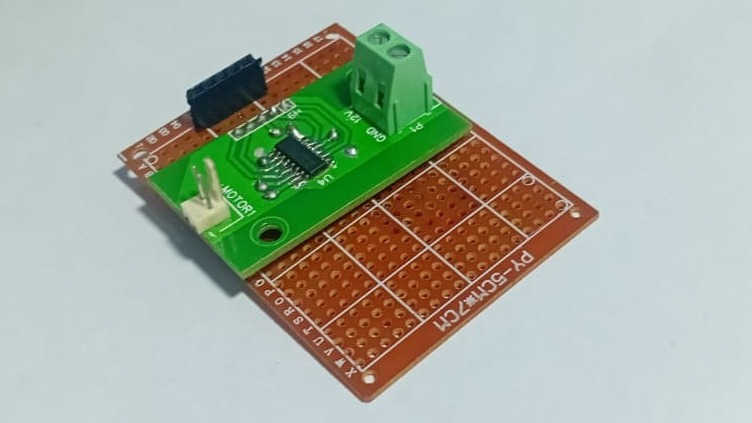
\includegraphics[width=\linewidth]{CHPTRS/CH07_IMPLEMENTACION/Fig/VNH.jpeg}
    \caption{Implementación física del \textit{driver} VNH7070BAS en una placa de pruebas.}
    \label{fig:vnh_pcb_impl}
  \end{subfigure}

  \caption{Implementación de prueba del \textit{driver} VNH7070BAS.}
  \label{fig:vnh_pcb_poc}
  \caption*{\footnotesize\textit{Nota: Componentes cortesía del profesor Enrique Vidal.}}
\end{figure}

\noindent
Una vez obtenida la \ac{PCB} de pruebas, se comenzó a realizar la conexión con los pines asignados para el control del driver del motor, con el objetivo de obtener los parámetros de voltaje y corriente que llegan al motor. Para la medición del voltaje del motor, se emplea un divisor de tensión conectado a la entrada del voltaje nominal. Esto se debe a que el microcontrolador seleccionado cuenta con un ADC que opera en el rango de \SIrange{0}{3.3}{\volt}. 
De manera similar a las pruebas del sensor Hall, se presentan los resultados del sensado de las variables medidas. En la Figura~\ref{fig:graph_voltaje} se muestra el registro de la tensión de la fuente de alimentación del motor, correspondiente a \SI{12}{\volt} nominal.

% ---------------------------------------------------------
% Figura: sensado de voltaje
% ---------------------------------------------------------
\begin{figure}[ht!]
\centering
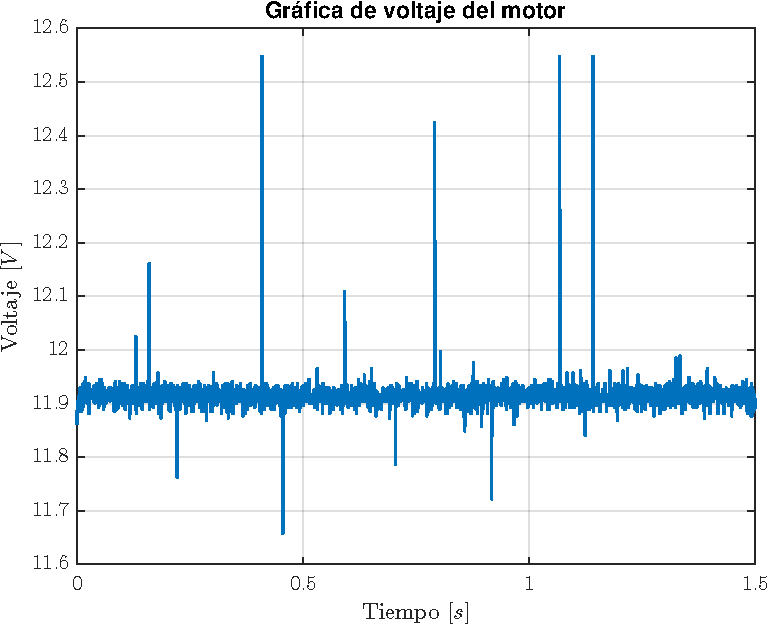
\includegraphics[width=0.70\linewidth]{CHPTRS/CH07_IMPLEMENTACION/Fig/voltaje_graph.pdf}
\caption{Señal de voltaje de alimentación del motor obtenida durante las pruebas.}
\label{fig:graph_voltaje}
\end{figure}

\noindent
En cuanto a la corriente, se presentan dos registros. Para estas pruebas, se diseñó el circuito de adecuación de señal de voltaje que permite medir la corriente de los motores evaluados; sin embargo, esta medición se realiza a partir de una ganancia de escalamiento $K$ que relaciona la corriente real del motor con la señal de sensado, la cual corresponde a un valor típico indicado en la hoja de datos \autocite{ST_VNH7070BAS}, tal como se describe en la sección \ref{sec:diseno_filtros_sensado} del Anexo \ref{an:Anexo_u}. Debido a que $K$ es un valor típico y puede variar según el motor sensado y sus parámetros eléctricos (por ejemplo, resistencia e inductancia), es necesario emplear una pinza amperométrica para validar experimentalmente que la corriente medida por el sistema corresponde a la corriente real del motor. En la Figura~\ref{fig:graph_current_start} se muestra la toma de datos durante \SI{1.5}{\second}, en la cual se observa un pico de corriente al inicio debido a la inercia asociada al arranque del motor. Por otro lado, en la Figura~\ref{fig:graph_current_forced} se presenta un lapso de tiempo más prolongado, en el cual se forzó el eje del motor con el propósito de verificar la coherencia de la medición; bajo esta condición se espera un incremento de corriente para vencer la fuerza que restringe el giro del eje. En ambos casos, también se aprecia el ruido presente en la señal de corriente, la cual es adquirida por el microcontrolador como una medición de voltaje.


% ---------------------------------------------------------
% Figura con dos subfiguras: corriente normal y corriente forzada
% ---------------------------------------------------------
%---------------------------------------------------------
% Figura: corriente durante arranque (1.5 s)
%---------------------------------------------------------
\begin{figure}[H]
\centering
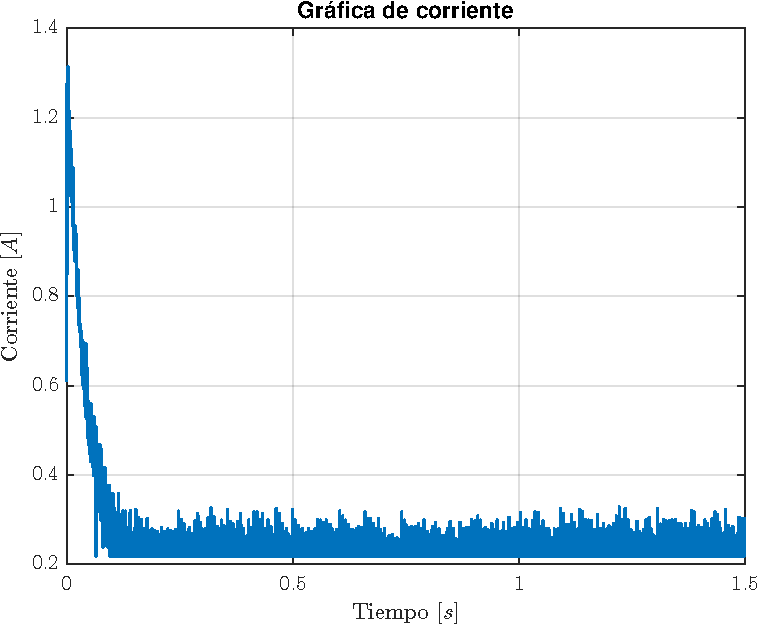
\includegraphics[width=0.80\linewidth]{CHPTRS/CH07_IMPLEMENTACION/Fig/corriente_graph.pdf}
\caption{Corriente durante el arranque del motor (\SI{1.5}{\second}).}
\label{fig:graph_current_start}
\end{figure}

%---------------------------------------------------------
% Figura: corriente con eje forzado
%---------------------------------------------------------
\begin{figure}[H]
\centering
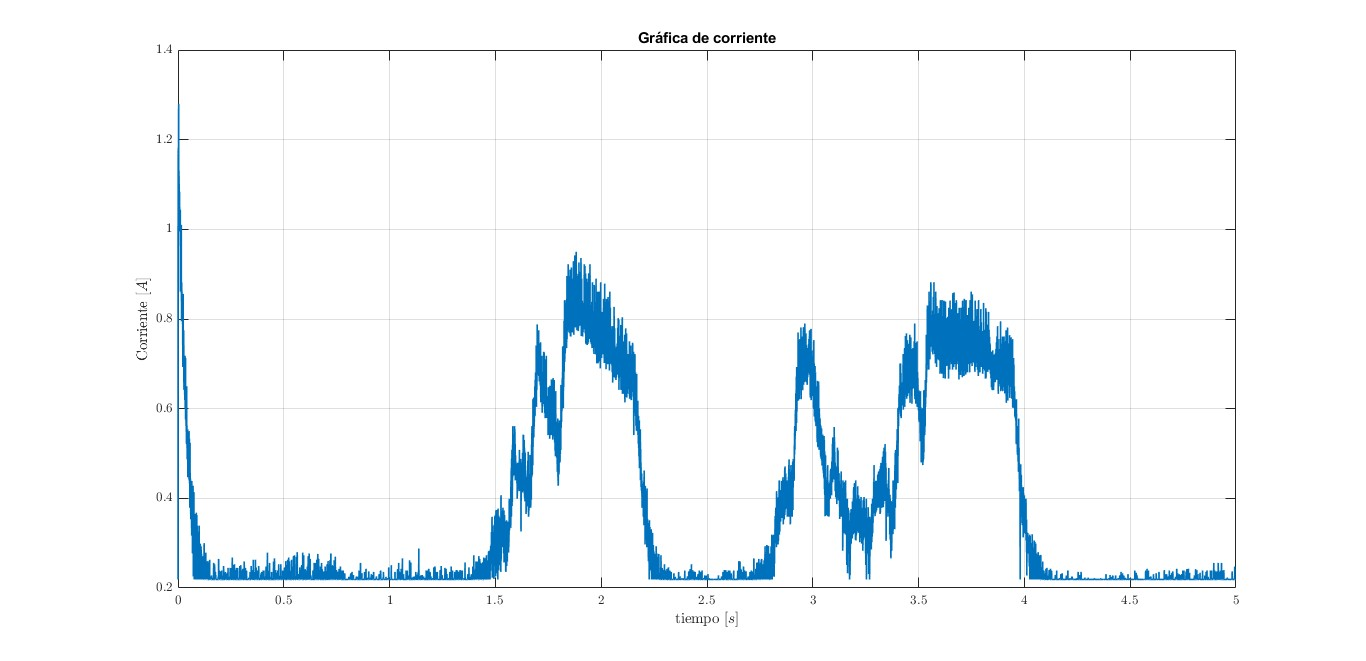
\includegraphics[width=\linewidth]{CHPTRS/CH07_IMPLEMENTACION/Fig/corriente_graph_force.jpg}
\caption{Corriente con eje forzado durante un intervalo prolongado.}
\label{fig:graph_current_forced}
\end{figure}

\noindent
Para todas estas pruebas, tanto de voltaje como de corriente y velocidad angular, se trabajó con un periodo entre muestras de \SI{500}{\micro\second}, lo que equivale a una frecuencia de muestreo de \SI{2}{\kilo\hertz}. Este muestreo busca capturar adecuadamente el arranque del motor en pruebas de corta duración, debido a que la dinámica de estas variables es rápida y converge en un intervalo reducido, tal como se observa en las figuras presentadas. Por este motivo, se optó por una ventana de adquisición de aproximadamente \SI{1.5}{\second}, donde la información es almacenada en la memoria RAM del microcontrolador para luego ser enviada hacia la interfaz, en la cual se ejecutará el algoritmo de estimación. Para mayor detalle sobre la lógica de funcionamiento del sistema, esta se describe en el Capítulo~\ref{ch:CH06}, correspondiente al desarrollo de la lógica de control y \ac{SW}.


\section{Prueba de sensado utilizando el \ac{HW} implementado}

\noindent
Con el objetivo de validar el banco de pruebas, se realizaron pruebas experimentales utilizando motores \ac{DC} comerciales de \SI{12}{V}. Llos motores que se probarán a continuación no cuentan con una ficha técnica. Es por ello, que la obtención de sus parámetros eléctricos y mecánicos deberá realizarse mediante comparación entre los métodos empíricos descritos en el Anexo \ref{an:Anexo_C} y el método de estimación paramétrica propuesto en este trabajo.
\noindent
Los motores utilizados corresponden a los modelos JGB37 y JGA25, cuya nomenclatura hace referencia al diámetro externo del cuerpo del motor (\SI{37}{mm} y \SI{25}{mm}, respectivamente), dimensión relevante para el diseño mecánico del sistema de acople. Ambos motores fueron montados sobre perfiles de aluminio V-SLOT utilizando un \textit{bracket} diseñado con su geometría específica para garantizar su sujeción en la toma de datos. A continuación, en la Figura \ref{fig:motores_prueba} se presentan las fotos con los motores mencionados sujetos al perfil.

\begin{figure}[!ht]
    \begin{tabularx}{\linewidth}{*{2}{>{\centering\arraybackslash}X}}
        % FILA-1 (IMÁGENES)
        \begin{subfigure}[t]{0.45\textwidth}
            \centering
            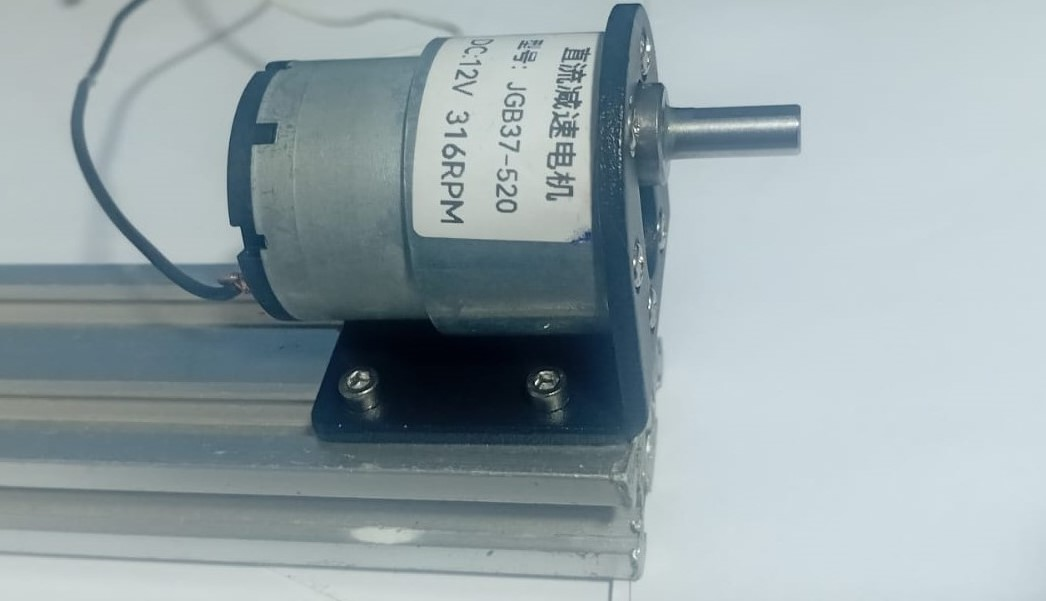
\includegraphics[width=.9\linewidth]{CHPTRS/CH07_IMPLEMENTACION/Fig/MotorGB37.jpeg}
        \end{subfigure}
        &
        \begin{subfigure}[t]{0.45\textwidth}
            \centering
            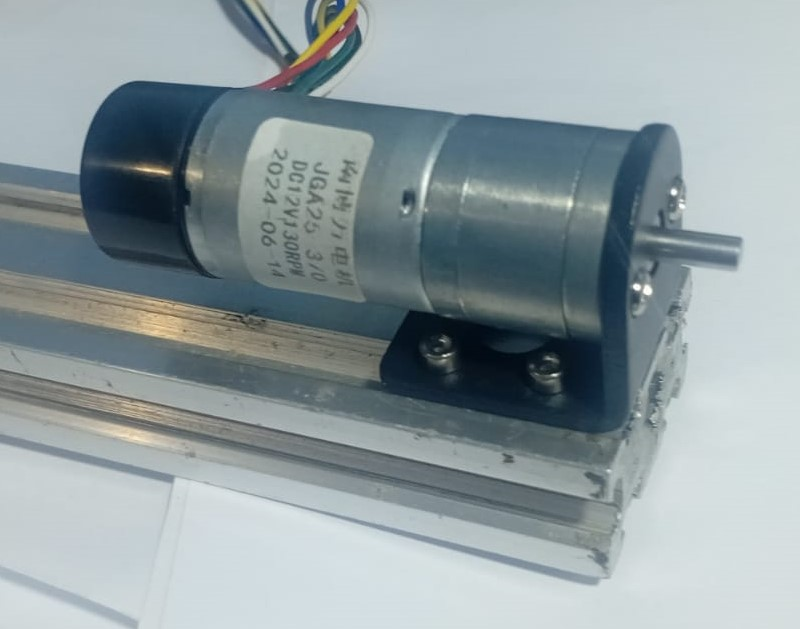
\includegraphics[width=.9\linewidth]{CHPTRS/CH07_IMPLEMENTACION/Fig/MOTORGA25.jpeg}
        \end{subfigure}
        \\ 
        % FILA-2 (CAPTIONS + LABELS)
        \begin{subfigure}[t]{0.9\linewidth}
            \caption{Motor \ac{DC} JGB37 de \SI{37}{mm} de diámetro, montado sobre perfil de aluminio mediante soporte impreso en 3D.}
            \label{fig:motor_jgb37}
        \end{subfigure}
        &
        \begin{subfigure}[t]{0.9\linewidth}
            \caption{Motor \ac{DC} JGA25 de \SI{25}{mm} de diámetro, acoplado al sistema de pruebas.}
            \label{fig:motor_jga25}
        \end{subfigure}
    \end{tabularx}
    \caption{Motores \ac{DC} utilizados para las pruebas experimentales de sensado.}
    \label{fig:motores_prueba}
\end{figure}
\noindent
Durante las pruebas iniciales se observó la necesidad de aplicar filtros para el tratamiento de los datos recolectados, especialmente en el sensado de la velocidad angular, debido a la presencia de ruido de medición y pequeñas oscilaciones por no haber sujetado correctamente el sensor de efecto \textit{hall}. En laa Figura \ref{fig:velocidades_prueba} se muestran los resultados de la medición de esta variable, que ejemplifica cómo es que influye que el imán de neodimio y el sensor estén lo más centrados posible.

\begin{figure}[!ht]
    \begin{tabularx}{\linewidth}{*{2}{>{\centering\arraybackslash}X}}
        % FILA-1 (IMÁGENES)
        \begin{subfigure}[t]{0.45\textwidth}
            \centering
            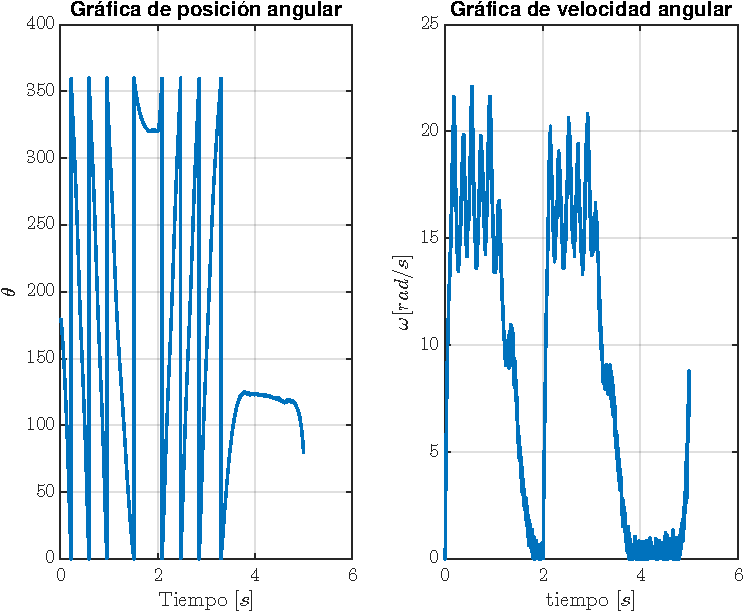
\includegraphics[width=.95\linewidth]{CHPTRS/CH07_IMPLEMENTACION/Fig/w_JGB37.pdf}
        \end{subfigure}
        &
        \begin{subfigure}[t]{0.45\textwidth}
            \centering
            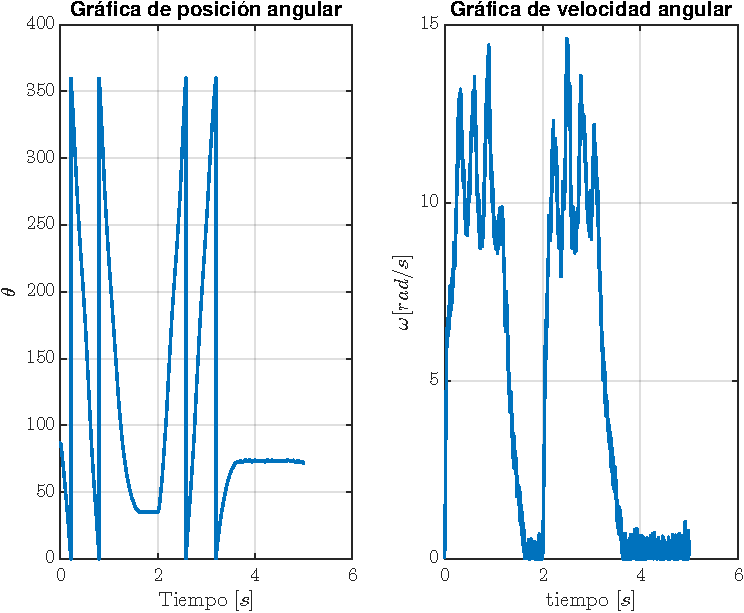
\includegraphics[width=.95\linewidth]{CHPTRS/CH07_IMPLEMENTACION/Fig/w_JGA25.pdf}
        \end{subfigure}
        \\ 
        % FILA-2 (CAPTIONS + LABELS)
        \begin{subfigure}[t]{0.9\linewidth}
            \caption{Respuesta de velocidad angular del motor JGB37 ante señal de prueba.}
            \label{fig:omega_jgb37}
        \end{subfigure}
        &
        \begin{subfigure}[t]{0.9\linewidth}
            \caption{Respuesta de velocidad angular del motor JGA25 ante señal de prueba.}
            \label{fig:omega_jga25}
        \end{subfigure}
    \end{tabularx}
    \caption{Curvas experimentales de velocidad angular registradas durante el sensado.}
    \label{fig:velocidades_prueba}
\end{figure}

\section{Pruebas con la interfaz}
\noindent
En esta sección se muestran las interacciones básicas del usuario con la interfaz desarrollada. En primer lugar, como se mencionó en el Capítulo \ref{ch:CH06} es necesario que el usuario identifique correctamente el puerto de comunicación al que se encuentra conectado el microcontrolador, ya que la transmisión de datos entre la interfaz y el microcontrolador depende directamente de esta configuración.
\noindent
La Figura \ref{fig:acceso_com} muestra,  cómo acceder a la información del sistema para identificar el puerto asignado y copiar el valor correspondiente. Mientras que en la Figura \ref{fig:error_com} se presenta el mensaje de error que aparece cuando se ingresa un puerto incorrecto o inválido, impidiendo la comunicación entre la interfaz y el microcontrolador.

\begin{figure}[!ht]
    \begin{tabularx}{\linewidth}{*{2}{>{\centering\arraybackslash}X}}
        % FILA-1 (IMÁGENES)
        \begin{subfigure}[t]{0.45\textwidth}
            \centering
            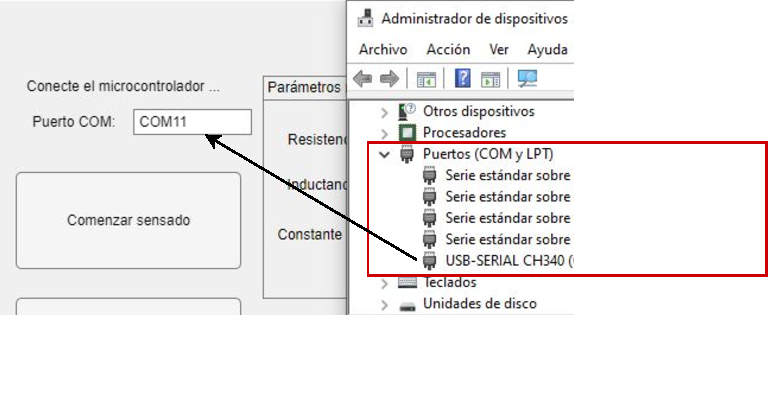
\includegraphics[width=.95\linewidth]{CHPTRS/CH07_IMPLEMENTACION/Fig/1_COM.pdf}
        \end{subfigure}
        &
        \begin{subfigure}[t]{0.45\textwidth}
            \centering
            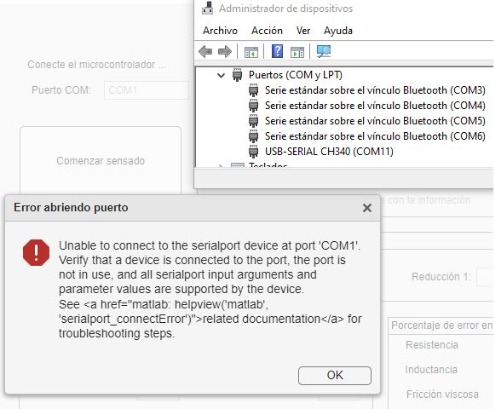
\includegraphics[width=.95\linewidth]{CHPTRS/CH07_IMPLEMENTACION/Fig/2_ERROR_COM.jpg}
        \end{subfigure}
        \\
        % FILA-2 (CAPTIONS + LABELS)
        \begin{subfigure}[t]{0.9\linewidth}
            \caption{Identificación del puerto de comunicación asignado al microcontrolador.}
            \label{fig:acceso_com}
        \end{subfigure}
        &
        \begin{subfigure}[t]{0.9\linewidth}
            \caption{Mensaje de error mostrado al ingresar un puerto incorrecto.}
            \label{fig:error_com}
        \end{subfigure}
    \end{tabularx}
    \caption{Configuración inicial del puerto de comunicación.}
    \label{fig:puerto_com}
\end{figure}
\noindent
Posteriormente, la interfaz validará que el usuario haya completado correctamente los datos de entrada, tales como los parámetros reales de la hoja de datos, si se dispone de ellos, y la indicación de si el motor cuenta o no con caja reductora. En caso contrario, se presentan mensajes de advertencia como el mostrado en la Figura \ref{fig:errores_entrada}.

\begin{figure}[!ht]
    \centering
    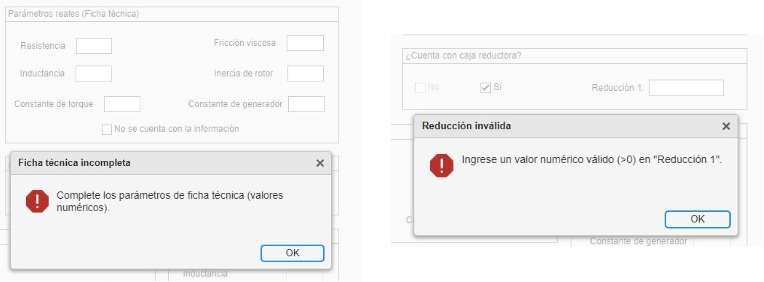
\includegraphics[width=0.7\textwidth]{CHPTRS/CH07_IMPLEMENTACION/Fig/3_ERRORES_INGRESO.jpg}
    \caption{Mensaje de advertencia cuando no se completan los datos requeridos por la interfaz.}
    \label{fig:errores_entrada}
\end{figure}
\noindent
Una vez configurado correctamente el puerto y completados los datos requeridos, se procede a iniciar el sensado. La Figura \ref{fig:sensado_correcto} muestra el funcionamiento adecuado de la comunicación entre la interfaz y el microcontrolador, donde se grafican en tiempo real las variables medidas del motor.

\begin{figure}[!ht]
    \centering
    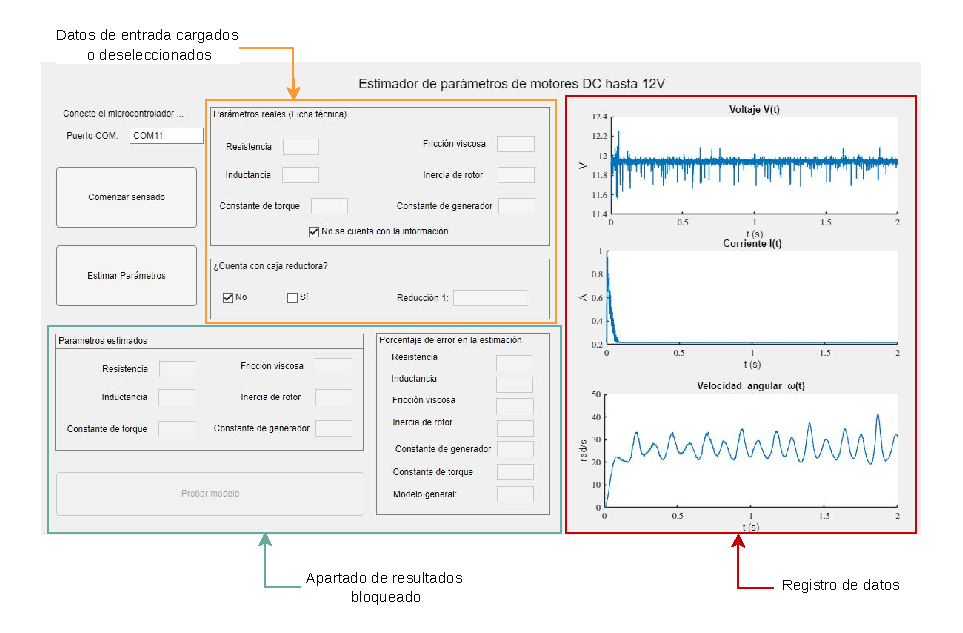
\includegraphics[width=0.9\textwidth]{CHPTRS/CH07_IMPLEMENTACION/Fig/4_FUNCIONAMIENTO-SENSADO.drawio.pdf}
    \caption{Visualización en tiempo real de las variables medidas durante el proceso de sensado.}
    \label{fig:sensado_correcto}
\end{figure}
\noindent
Luego de verificar que los datos adquiridos son coherentes, el usuario puede proceder a estimar los parámetros del motor. Para mayor detalle sobre el algoritmo utilizado, puede consultarse el Anexo \ref{an:Anexo_C}. La Figura \ref{fig:estimacion_resultados} muestra los resultados obtenidos tras ejecutar la estimación.

\begin{figure}[!ht]
    \centering
    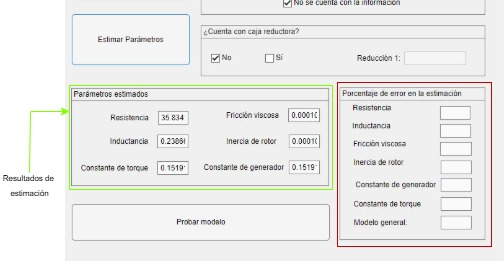
\includegraphics[width=0.9\textwidth]{CHPTRS/CH07_IMPLEMENTACION/Fig/5_Resultados.jpg}
    \caption{Resultados de la estimación paramétrica mostrados en la interfaz.}
    \label{fig:estimacion_resultados}
\end{figure}
\noindent
Si bien la interfaz cumple su función de presentar los resultados en las casillas respectivos, puede mejorarse en futuras iteraciones incorporando explícitamente las unidades correspondientes en el \ac{SI} junto a cada parámetro estimado, ya que no queda tan claro en qué unidades está la dimensional de los resultados, para saber las unidades de estos parámetros, esta información puede consultar en en el Anexo \ref{an:Anexo_E}.
\noindent
Posteriormente de presentar los resultados, se habilita la opción de probar el modelo con los parámetros estimados. En esta etapa se carga en el microcontrolador una rutina descrita en el Capítulo \ref{ch:CH06}, destinada a realizar una nueva toma de datos para la validación del modelo. Con los parámetros previamente estimados se construye un modelo ideal de la planta, cuya respuesta se grafica junto a las señales medidas, como se observa en la Figura \ref{fig:prueba_modelo}.

\begin{figure}[!ht]
    \centering
    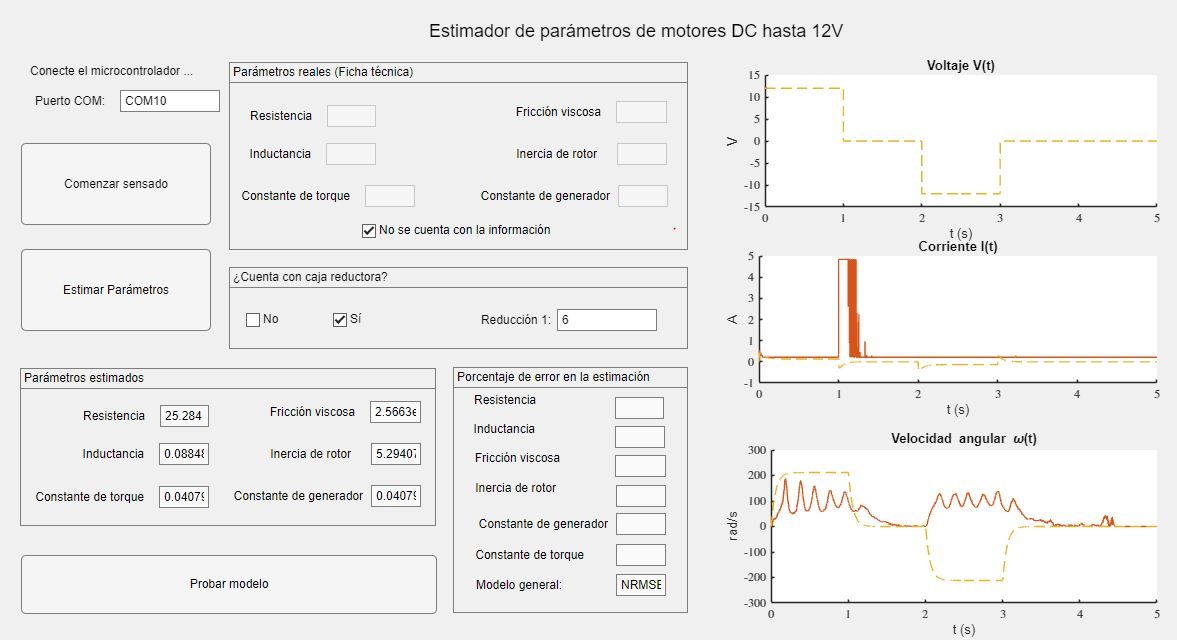
\includegraphics[width=0.9\textwidth]{CHPTRS/CH07_IMPLEMENTACION/Fig/6_Discución_final.JPG}
    \caption{Comparación entre la respuesta experimental y el modelo ideal construido con los parámetros estimados.}
    \label{fig:prueba_modelo}
\end{figure}
\noindent
Finalmente, durante las pruebas se identificó un comportamiento particular en el sensado. En el caso de la velocidad angular, se observa una oscilación alrededor de un punto de operación, lo cual indica la necesidad de aplicar un filtrado adicional para mejorar la calidad de la señal. Asimismo, en el sensado de corriente se evidencia un pico significativo cuando el motor es forzado a detenerse, tal como se aprecia en la Figura \ref{fig:pico_corriente}.

\begin{figure}[!ht]
    \centering
    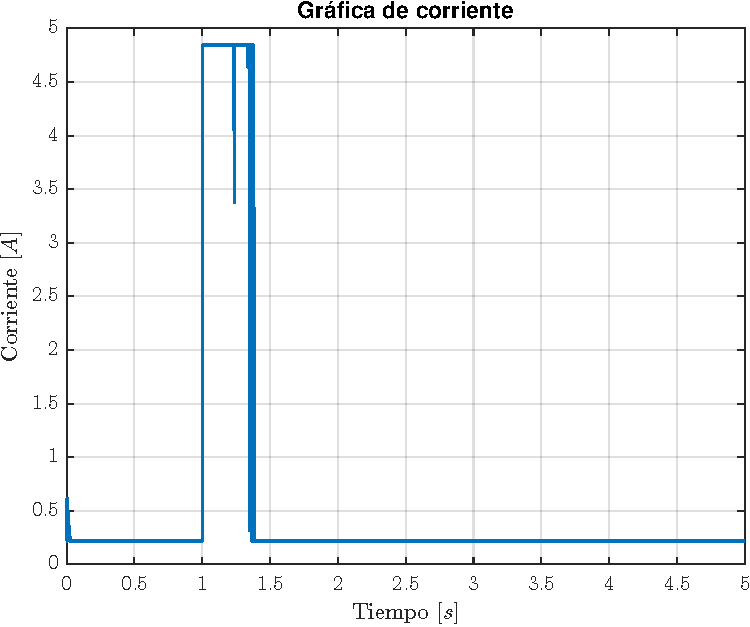
\includegraphics[width=0.9\textwidth]{CHPTRS/CH07_IMPLEMENTACION/Fig/7_Ayuda_discución_final.pdf}
    \caption{Pico de corriente registrado al forzar la detención del motor.}
    \label{fig:pico_corriente}
\end{figure}
\noindent
Este fenómeno sugiere que parte de la información podría no estar siendo capturada correctamente por el micrcontrolador. Como se mencionó en la sección \ref{sec:pruebas_driver}, se emplea una ganancia genérica para escalar la medición de corriente del motor. Es posible que esta configuración esté provocando saturación en el ADC del microcontrolador, impidiendo una medición precisa en condiciones transitorias abruptas. Este efecto introduce uu arrastre de error en el proceso de estimación y deberá analizarse con mayor detalle en futuras iteraciones del sistema.

 \cleardoublepage
\chapter{Costos de implementación}
\ihead[]{Capítulo 8: Costos de implementación}
\label{ch:CH08-Costos}
%%%%%%%%%%%%%%%%%%%%%%%%%%%%%%%%%%%%%%%%%%
Se analizarán todo los costos que se requerirá para obtener el prototipo funcional
\section{Costo de componentes}
\section{Costo de diseño y fabricación}
\section{Costo total}               \cleardoublepage
\addchap{Conclusiones y Trabajo Futuro}
\ihead[]{Conclusiones y Trabajo Futuro}
\label{ch:CH09}
%%%%%%%%%%%%%%%%%%%%%%%%%%%%%%%%%%%%%%%%%%
% Conclusiones y Recomendaciones
\noindent
Para finalizar este trabajo de investigación, se presentan las observaciones y conclusiones obtenidas a lo largo del desarrollo de este, las cuales no solo evidencian que los principales objetivos del diseño conceptual fueron alcanzados, sino que también destacan el aprendizaje sobre motores \ac{DC}.
\section*{Conclusiones}
\begin{itemize}

\item Se culminó el diseño conceptual del sistema mediante la integración de los subsistemas mecánico, electrónico y de \ac{SW}, realizando pruebas con \ac{HW} físico que permitieron validar las funcionalidades del banco de pruebas. Sin embargo, se identificó que el algoritmo de estimación aún puede ser perfeccionado, particularmente en el tratamiento del ruido de medición y dar resultados concluyentes de los motores. Por ello, si bien el diseño conceptual y su validación experimental han sido completados, se requiere continuar iterando el desarrollo del algoritmo para mejorar la precisión y confiabilidad de los parámetros estimados.

\item El análisis económico realizado demuestra que la viabilidad económica del banco de pruebas depende directamente del escenario de implementación considerado. Si se contemplan todos los costos asociados al desarrollo incluyendo diseño, licencias de \ac{SW} e importaciones, el monto total supera ampliamente el requerimiento presupuestal establecido. No obstante, al restringir el análisis a los costos reales de fabricación e implementación física del sistema, se obtiene un valor que se mantiene dentro del margen de S/.1000, incluso considerando la importación de los componentes electrónicos principales. Esto evidencia que la solución propuesta es técnicamente viable y económicamente competitiva cuando se separan los costos de desarrollo de los costos de reproducción del prototipo.

\end{itemize}
\section*{Trabajo Futuro}

\begin{itemize}

\item Debido a limitaciones en los instrumentos de medición disponibles durante el desarrollo del proyecto, particularmente en el sensado de corriente con una pinza amperométrica, se trabajó con una ganancia genérica para escalar la señal de corriente, convertida en voltaje por la resistencia $R_{sense}$, brindada por el fabricante del \textit{driver} de motor. Como trabajo futuro, se recomienda realizar un proceso de calibración experimental del sistema de medición de corriente, empleando instrumentos de mayor precisión para hallar el valor más preciso de esta ganancia, ya que, como se pudo evidenciar en el Capítulo \ref{ch:CH07}, hubo mediciones no tan precisas al momento de ejecutar la rutina para la prueba del modelo estimado. 

\item En el análisis económico se identificó que varios de los componentes principales del sistema, como el \textit{driver} de motor y el sensor de efecto \textit{hall}, no se encuentran disponibles en el mercado local, por lo que deben ser importados desde proveedores internacionales. Como mejora futura, se recomienda evaluar alternativas tecnológicas disponibles en el mercado nacional que puedan cumplir con las mismas funciones que los componentes importados para cumplir efectivamente con el requerimiento de usuario referente a los costos, así como acuerdos con proveedores que permitan reducir costos de importación. Asimismo, se observó que, si bien la fabricación 

\item En cuanto al desarrollo de \ac{SW}, se recomienda migrar la aplicación de estimación de parámetros a lenguajes de programación de código abierto, como Python. Como se analizó en el Capítulo \ref{ch:CH08}, el uso de MATLAB implica costos significativos por licencias y \textit{toolboxes}. Una implementación en \ac{SW} libre además de reducir la inversión necesaria para replicar el banco de pruebas, permitiría integrar una \ac{GUI} más intuitiva y optimizada para el registro de resultados. Asimismo, es necesario seguir realizando más validaciones mediante ensayos con una mayor variedad de motores que cuenten con fichas técnicas de fabricante, con el fin de realizar una comparación de precisión entre los algoritmos de estimación propuestos y los métodos empíricos tradicionales.

\item Respecto al diseño del \ac{HW} mecánico, se plantea como mejora la adaptación del sistema de sujeción para motores de dimensiones reducidas o geometrías no convencionales. Si bien los perfiles V-SLOT actuales proporcionan un buen ajuste para carcasas cilíndricas de 12V, motores más pequeños o con formas irregulares requieren otros componentes de fijación. Se sugiere investigar el uso de nuevos perfiles que aseguren la estabilidad mecánica y la correcta alineación de estos motores durante el proceso de caracterización.

\item Para optimizar la calidad del sensado de las variables físicas, se requiere mejorar la precisión en el montaje del sistema de medición angular. Se observó que la coaxialidad entre el imán acoplado al eje y el sensor de efecto \textit{hall} es determinante para obtener lecturas de velocidad estables y sin ruido excesivo. Como trabajo futuro, se recomienda, igualmente, realizar pruebas adicionales mediante prototipado rápido para diseñar un acople centrado que garantice que el imán se mantenga en la posición óptima respecto al integrado. Esto, sumado a la implementación de filtros digitales ayudará para mejorar la estimación.

\end{itemize}

% \section{Conclusiones}

% \begin{itemize}

% \
% \end{itemize}            \cleardoublepage 

\printbibliography[heading=bibintoc,title={Bibliografía}]
\ihead[]{Bibliografía}
\cleardoublepage
% %%%%%%% Anexos y Acrónimos
\appendix
%%%%%%%%% ANNEX A
\chapter{Acr\'onimos}
\label{an:Annex_A_Acronimos}
Acrónimos usados en el presente trabajo de investigación:
\begin{acronym}[ABCDEFGHIJK]
%A
\acro{AF}{alta frecuencia}
%B
\acro{BF}{baja frecuencia}

%c
\acro{CoS}{concepto de solución}
%\ac{API}
%D
\acro{DC}{\textit{Direct Current}} %\ac{DC}
%E
\acro{ETAP}{\textit{Electrical Transient and Analysis Program}}
%F
\acro{FEM}{Fuerza contraelectromotriz}
\acro{FPGA}{\textit{Field-Programmable Gate Array}}
%G
\acro{GUI}{\textit{Graphical User Interface}}
%H
\acro{HW}{Hardware} %\ac{HW}
%M
\acro{MEE}{Modelo de Espacio de Estados}
\acro{MIMO}{\textit{Multiple Input Multiple Output}}
\acro{MCB}{\textit{Motor Control Blockset}}
\acro{MQTT}{\textit{Message Queuing Telemetry Transport}}
%N
\acro{TRL}{\textit{Technological Readiness Level}}
%P
\acro{PC}{\textit{Personal Computer}}
\acro{PCB}{\textit{Printed Circuit Board}}
\acro{PUCP}{Pontificia Universidad Católica del Perú}

%S
\acro{SW}{Software}
\acro{SWA}{Software A}
\acro{SWB}{Software B}
\acro{SISO}{\textit{Single Input Single Output}}
\acro{SBC}{\textit{Single Board Computer}}
%T
\acro{TFC1}{Trabajo de Fin de Carrera 1}
\acro{TFC2}{Trabajo de Fin de Carrera 2}
\end{acronym}    
\cleardoublepage 
%%%%%%%%% ANNEX B
\chapter{Tabla de variables}
\label{an:Annex_B_TablaVaribles}
Tabla de variables utilizadas:
\begin{table}[h!]
    \centering
    \caption{Tabla de variables del modelo de motor DC}
    \begin{tblr}{|c|c|c|}
        \hline
        \textbf{Símbolo} & \textbf{Descripción} & \textbf{Unidades} \\ \hline
        $u(t)$ & Voltaje de entrada & V (voltios) \\ \hline
        $i(t)$ & Corriente del motor & A (amperios) \\ \hline
        $R$ & Resistencia del rotor y las escobillas & $\Omega$ (ohmios) \\ \hline
        $L$ & Inductancia del motor & H (henrios) \\ \hline
        $u_a(t)$ & Fuerza contraelectromotriz (FEM) & V (voltios) \\ \hline
        $\omega(t)$ & Velocidad angular & rad/s (radianes por segundo) \\ \hline
        $\tau(t)$ & Par motor & N·m (newton-metro) \\ \hline
        $J$ & Inercia del motor & kg·m$^2$ \\ \hline
        $\mu$ & Coeficiente de fricción viscosa & N·m·s/rad \\ \hline
        $T_L$ & Par de carga externa & N·m (newton-metro) \\ \hline
        $K_e$ & Constante de tensión (FEM) & V·s/rad \\ \hline
        $K_t$ & Constante de par & N·m/A \\ \hline
    \end{tblr}
    \label{tab:Annex_B_variables}
\end{table}




\cleardoublepage
%%%%%%%%% ANNEX C
\chapter{Precio del software A}
\label{an:Anexo_C_Precios}
\label{an:matlab_prices}
Se presentarán los precios por adquirir una licencia de MATLAB según la su página oficial \textcite{ej-10-cita-pag-web} (Consultada el DD de MM del AAAA).
\\
En la Figura~\ref{fig:Annex_C_precio_sw} se presenta el precio de la licencia para estudiantes.
\begin{figure}[H]
        \centering       
        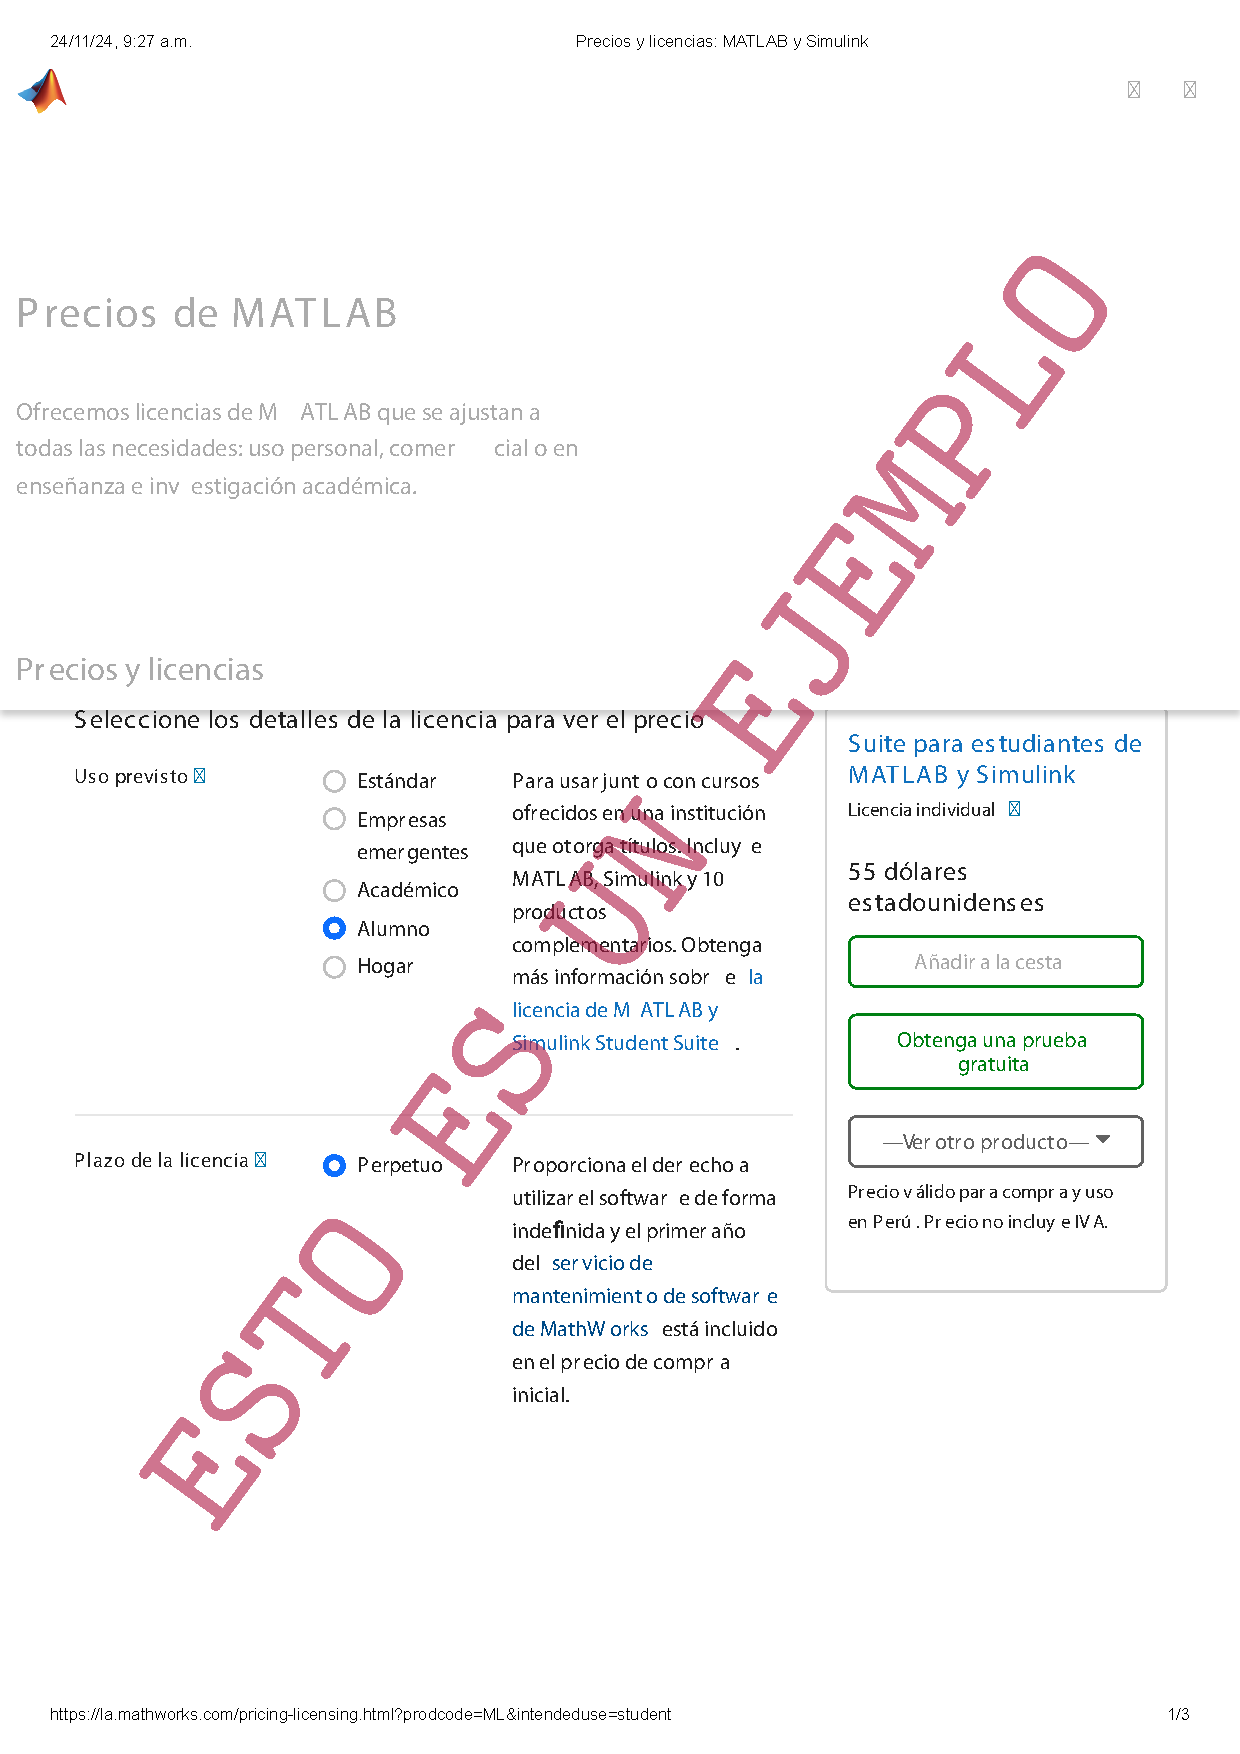
\includegraphics[width=0.6\textwidth]{ANNEX/Fig/AC_Precios-licencias-SW.pdf}
        \caption{Ejemplo correo de cotización}
        \caption*{\small\textit{Nota: Consultado el día DD de MM de AAAA}}
        \label{fig:Annex_C_precio_sw}
\end{figure}

     
\cleardoublepage
%%%%%%%%% ANNEX D
\chapter{Estructura de funciones completa}
\label{an:Anexo_D_Estructura-Funciones}
Las funciones del sistema serán agrupadas y organizadas según el dominio al que pertenecen, para facilitar la comprensión global del funcionamiento del sistema a diseñar. 
\begin{figure}[H]
        \centering       
        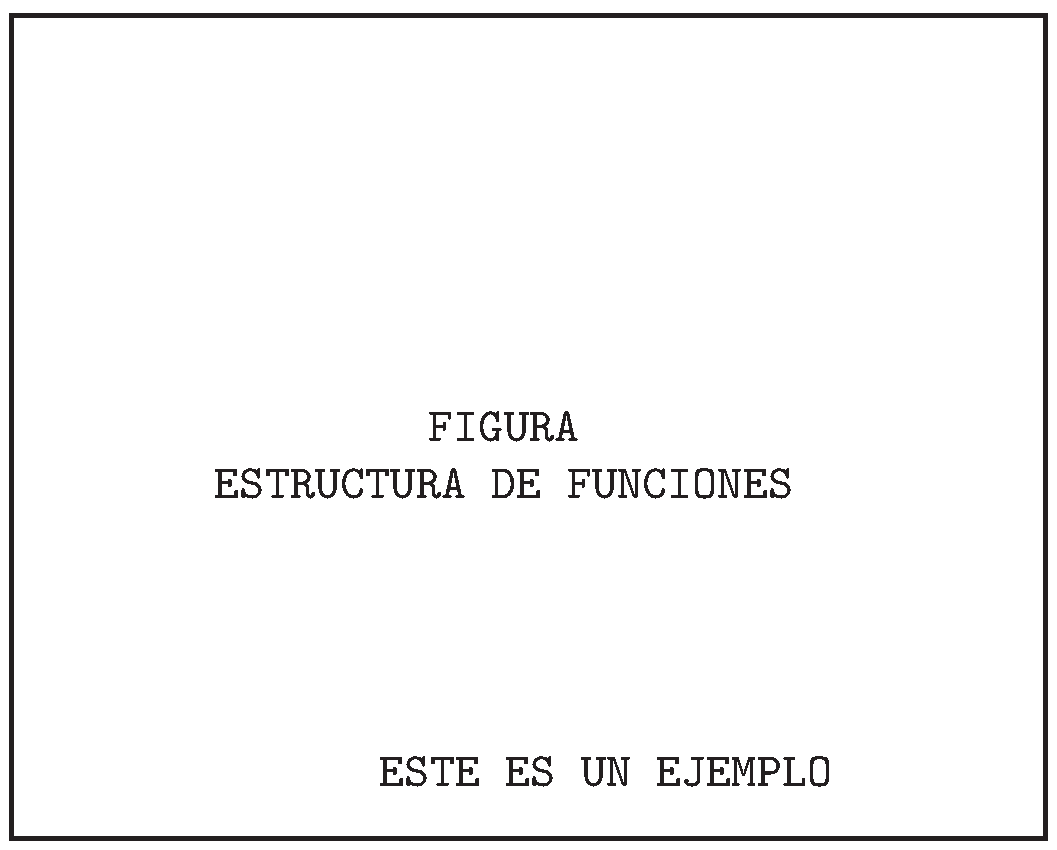
\includegraphics[width=1\textwidth]{ANNEX/Fig/AD_01-Estructura-de-funciones-sample.pdf}
        \caption{Estructura de funciones}
        \label{fig:Annex_D_Estructura_func}
    \end{figure}
\cleardoublepage
%%%%%%%%% ANNEX E
\chapter{Matriz morfológica}
\label{an:Anexo_E_MatrizMorfologica}
Se presentarán las matrices morfológicas de cada uno de los dominios y cómo se conectan para dar formas a los 3 conceptos de solución.
%%% FIGURA LEYENDA
\begin{figure}[H]
        \centering       
        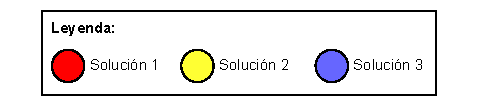
\includegraphics[width=0.4\textwidth]{ANNEX/Fig/AE_0-Leyenda.pdf}
        \label{fig:Annex_E_Leyenda}
\end{figure}
%%% FIGURA 1/7
\begin{figure}[H]
        \centering       
        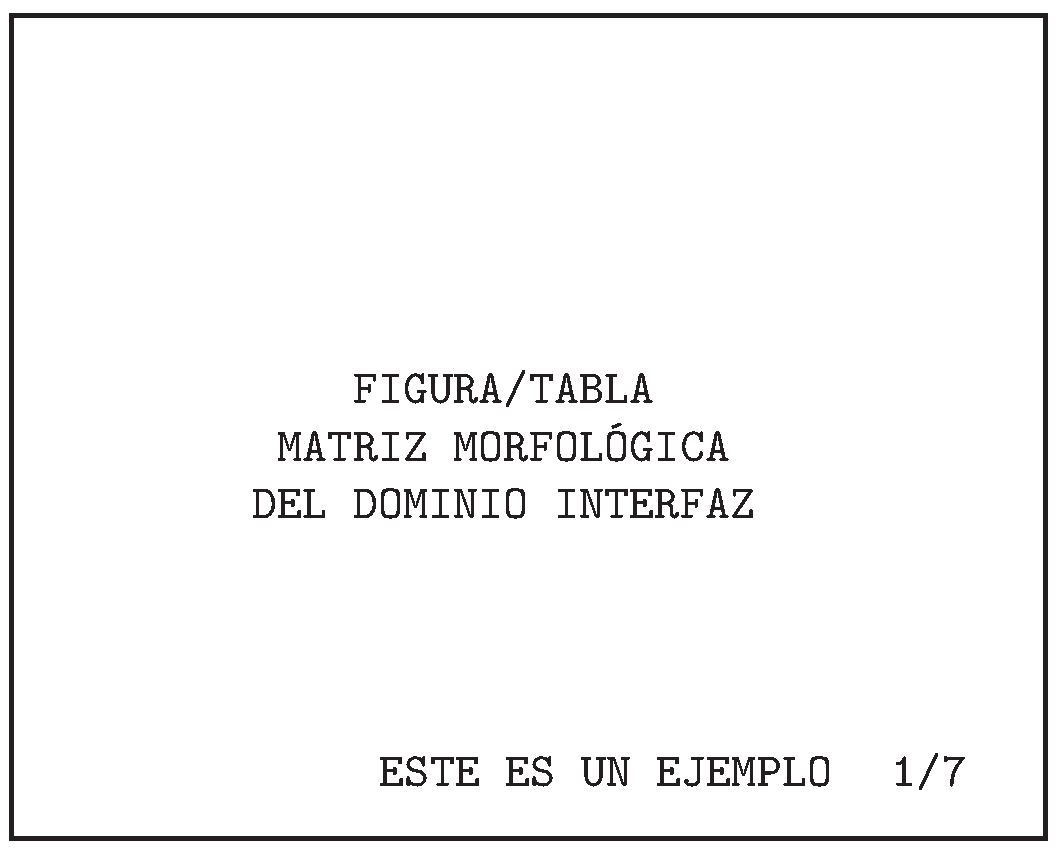
\includegraphics[width=0.7\textwidth]{ANNEX/Fig/AE_MatrizMorfologica-01-Dominio-Interfaz.pdf}
        \caption{Matriz morfológica para la interfaz del sistema}
        \label{fig:Annex_E_MatrizMorfologica-01-Interfaz}
\end{figure}
%%% FIGURA 2/7
\begin{figure}[H]
        \centering       
        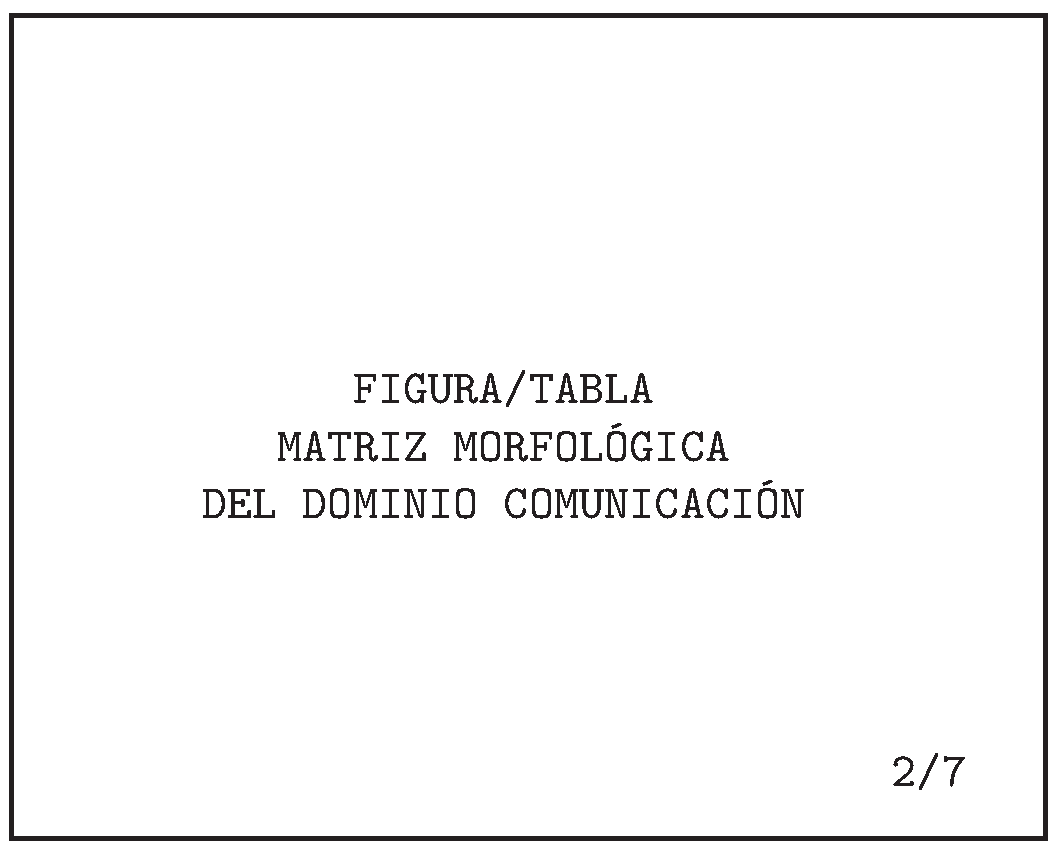
\includegraphics[width=0.7\textwidth]{ANNEX/Fig/AE_MatrizMorfologica-02-Dominio-Comunicacion.pdf}
        \caption{Matriz morfológica del dominio de comunicación}
        \label{fig:Annex_E_MatrizMorfologica-02-Comunicacion}
\end{figure}
%%% FIGURA 3/7
\begin{figure}[H]
        \centering       
        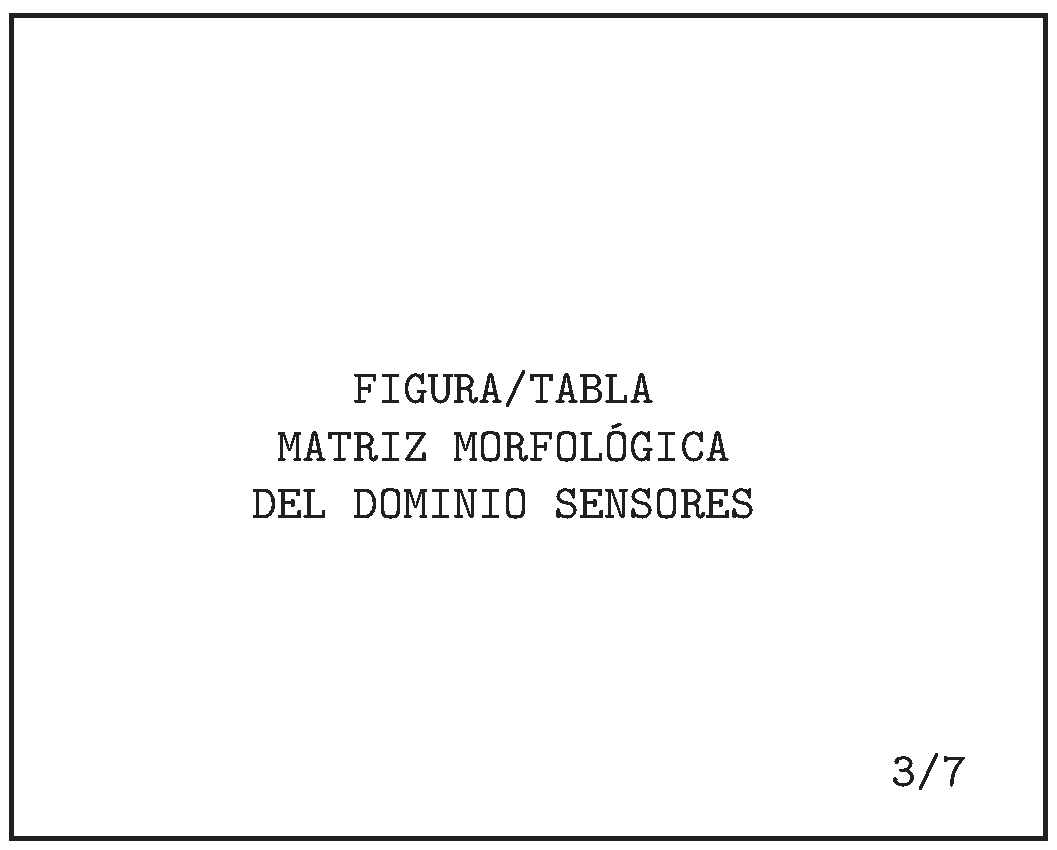
\includegraphics[width=0.7\textwidth]{ANNEX/Fig/AE_MatrizMorfologica-03-Dominio-Sensores.pdf}
        \caption{Matriz morfológica del dominio de sensores}
        \label{fig:Annex_E_MatrizMorfologica-03-Sensores}
\end{figure}
%%% FIGURA 4/7
\begin{figure}[H]
        \centering       
        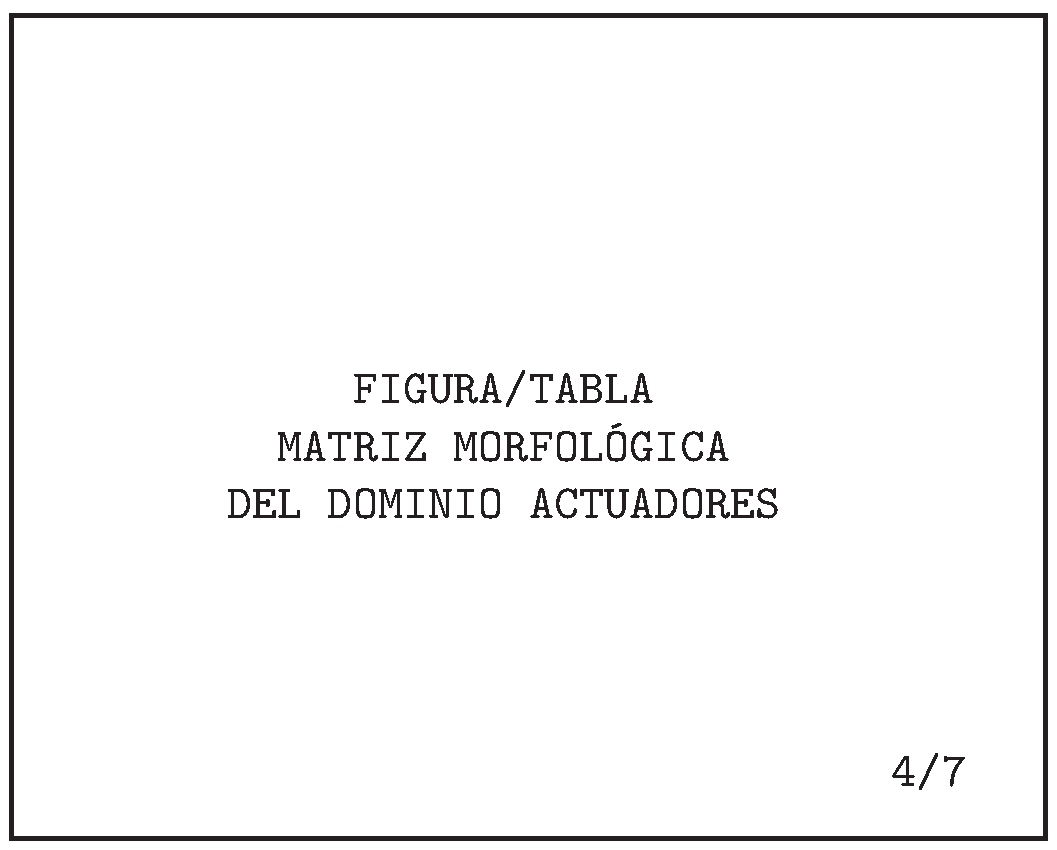
\includegraphics[width=0.7\textwidth]{ANNEX/Fig/AE_MatrizMorfologica-04-Dominio-Actuadores.pdf}
        \caption{Matriz morfológica del dominio de actuadores}
        \label{fig:Annex_E_MatrizMorfologica-04-Actuadores}
\end{figure}
%%% FIGURA 5/7
\begin{figure}[H]
        \centering       
        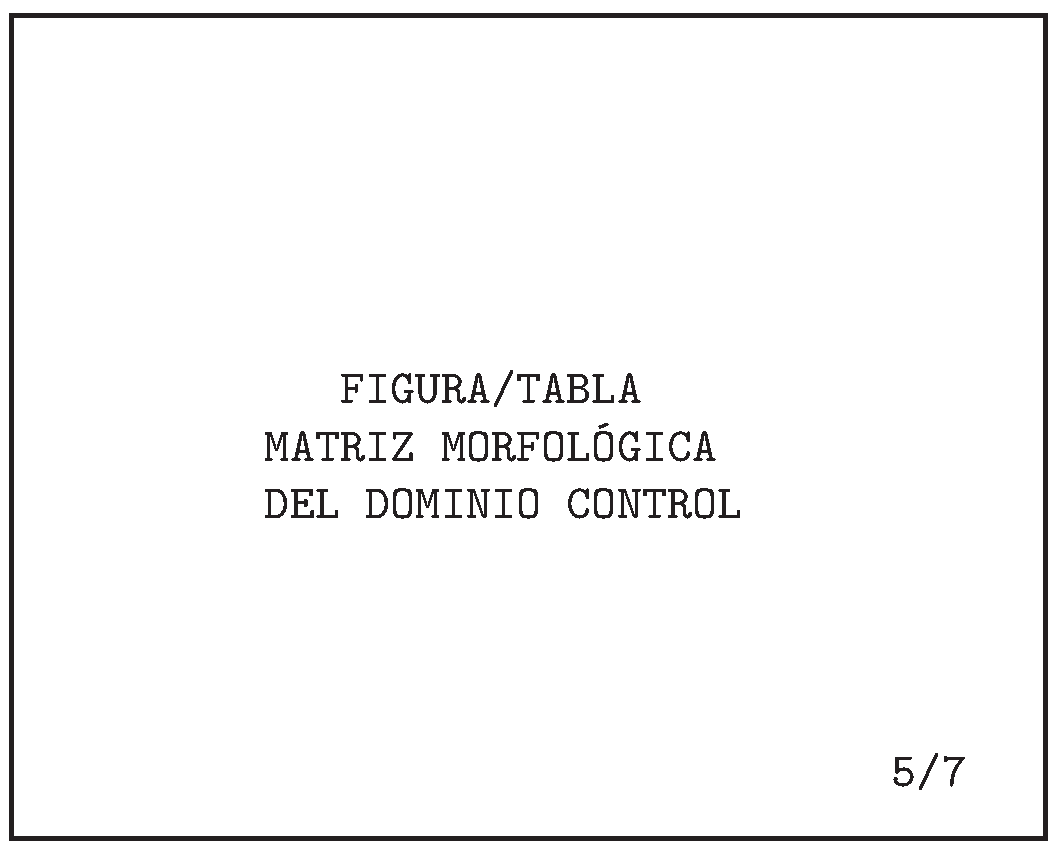
\includegraphics[width=0.7\textwidth]{ANNEX/Fig/AE_MatrizMorfologica-05-Dominio-Control.pdf}
        \caption{Matriz morfológica del dominio de control}
        \label{fig:Annex_E_MatrizMorfologica-05-control}
\end{figure}
%%% FIGURA 6/7
\begin{figure}[H]
        \centering       
        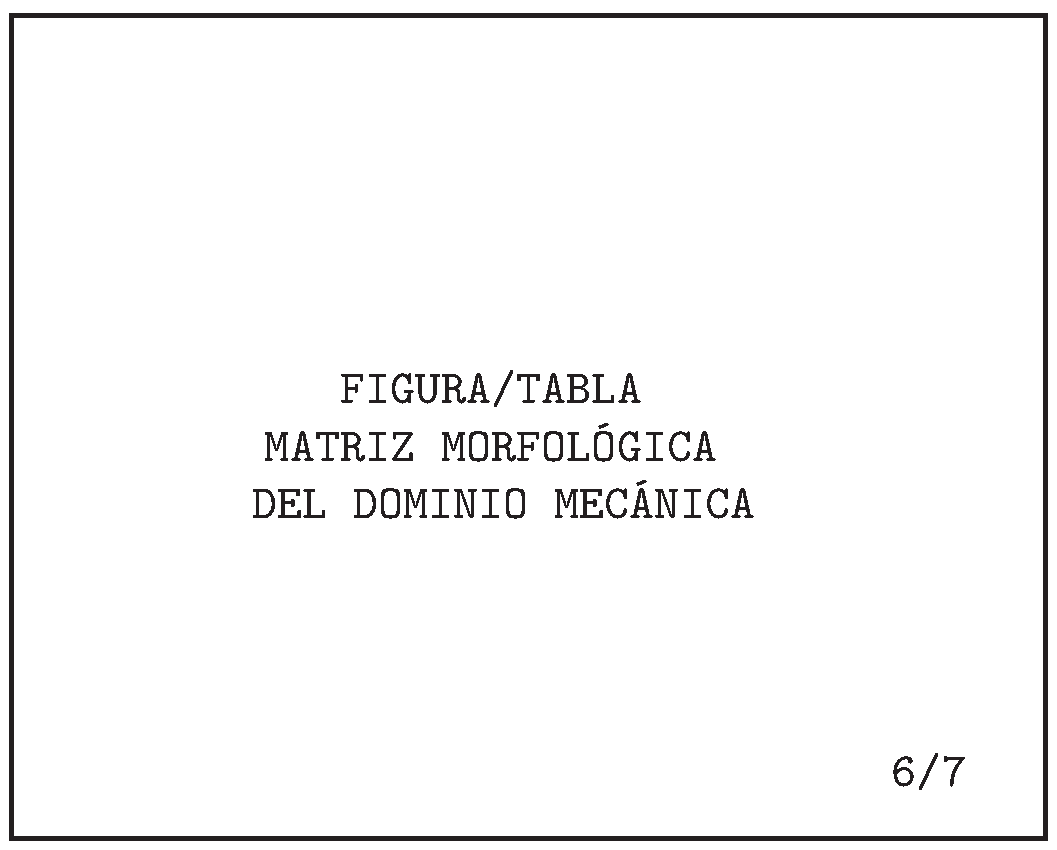
\includegraphics[width=0.7\textwidth]{ANNEX/Fig/AE_MatrizMorfologica-06-Dominio-Mecanica.pdf}
        \caption{Matriz morfológica del dominio de mecánica}
        \label{fig:Annex_E_MatrizMorfologica-06-Mecanica}
\end{figure}
%%% FIGURA 7/7
\begin{figure}[H]
        \centering       
        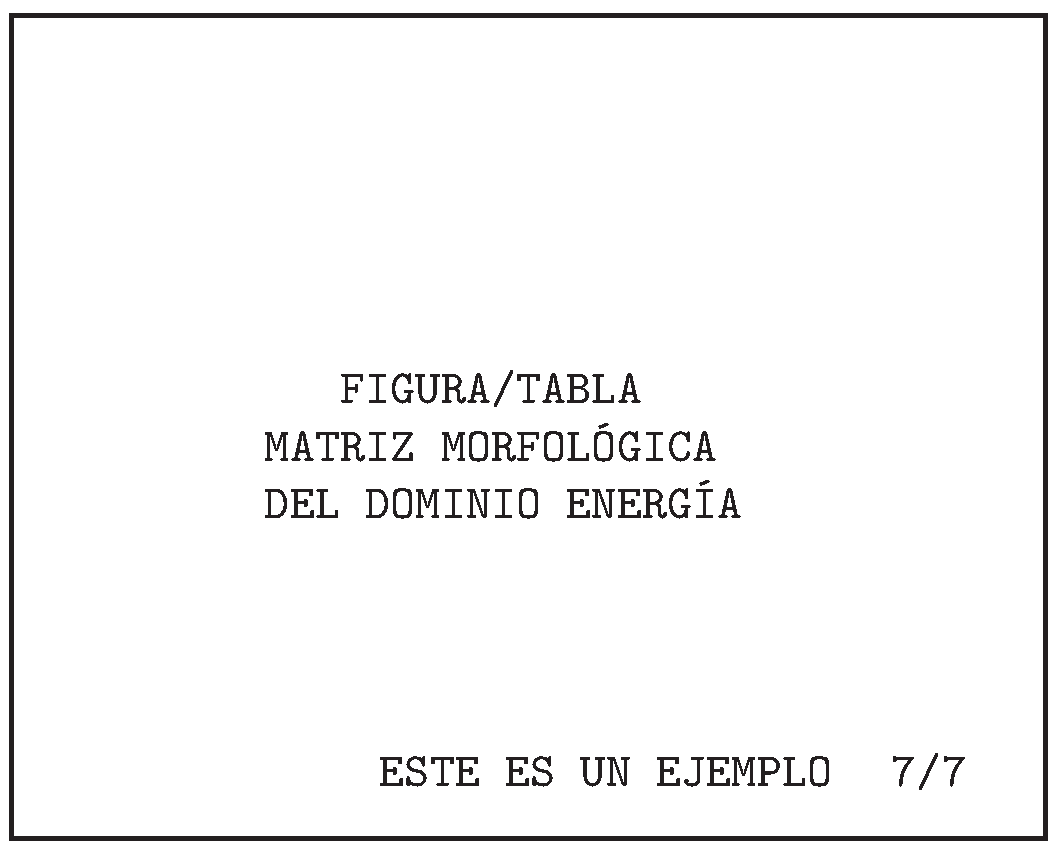
\includegraphics[width=0.7\textwidth]{ANNEX/Fig/AE_MatrizMorfologica-07-Dominio-Energia.pdf}
        \caption{Matriz morfológica del dominio de energía}
        \label{fig:Annex_E_MatrizMorfologica-07-Energia}
\end{figure}

\cleardoublepage

\end{document}